%%%%%%%%%%%%%%%%%%%%%%%%%%%%%%%%%%%%%%%%%%%%%%%%%%%%%%%%%%%%%%%%%%%%%%%%%%%%%
%%%%---------------------------------------------------------------------%%%%
%%%%%%%%%%%%%%%%%%%%%%%%%%%%%%%%%%%%%%%%%%%%%%%%%%%%%%%%%%%%%%%%%%%%%%%%%%%%%
\begin{frame}{Wave Models Under Study}
  Two more examples.
$$
$$

\onslide<1-2>{ The Benjamin-Ono equation:
\begin{equation}
u_t+u u_x - \mathcal{H} u_{xx}=0. \label{B-O}
\end{equation}

$$
\mathcal{H}u(x) = \frac{1}{\pi} p.v. \int_{-\infty}^{\infty}\frac{u(y)}{x -y} dy .
$$
}

\onslide<2-2>{The modified Benjamin-Ono equation:
\begin{equation}
u_t + u^2 u_x - \mathcal{H}  u_{xx}=0.
\end{equation}
}
\end{frame}
%%%%%%%%%%%%%%%%%%%%%%%%%%%%%%%%%%%%%%%%%%%%%%%%%%%%%%%%%%%%%%%%%%%%%%%%%%%%%
%%%%---------------------------------------------------------------------%%%%
%%%%%%%%%%%%%%%%%%%%%%%%%%%%%%%%%%%%%%%%%%%%%%%%%%%%%%%%%%%%%%%%%%%%%%%%%%%%%
\begin{frame}{Travelling Wave Solution}
 \onslide<1-2>{ A travelling wave solution to the equation 
\begin{equation*}
u_t+ f(u)_x + \Lop u_x=0 
\end{equation*}
is a function $$\phi(x-ct) := u(x,t)$$ 
with positive wave speed $c > 0$. 
}

\onslide<2-2>{
$ $ 

Travelling wave solutions exist if $f(u)$ and $\Lop$ satisfy some conditions. In particular:
\begin{itemize}
\item[*] $f(0) = f'(0) = 0.$

\item[*]	 $\Lop \mbox{ has a continuous, even, non-negative Fourier multiplier } \alpha(\cdot).$

\item[*] There is an $s > \frac{1}{2}$ such that $\lim_{k \rightarrow \infty} \inf |k|^{-s} \alpha(k) > 0.$
\end{itemize}

(ref. Hongqiu Chen, 2004)}
\end{frame}
%%%%%%%%%%%%%%%%%%%%%%%%%%%%%%%%%%%%%%%%%%%%%%%%%%%%%%%%%%%%%%%%%%%%%%%%%%%%%
%%%%---------------------------------------------------------------------%%%%
%%%%%%%%%%%%%%%%%%%%%%%%%%%%%%%%%%%%%%%%%%%%%%%%%%%%%%%%%%%%%%%%%%%%%%%%%%%%%

\section{Numerical Method}
\subsection{Pseudo-spectral scheme: Cosine collocation method}
%%%%%%%%%%%%%%%%%%%%%%%%%%%%%%%%%%%%%%%%%%%%%%%%%%%%%%%%%%%%%%%%%%%%%%%%%%%%%
%%%%---------------------------------------------------------------------%%%%
%%%%%%%%%%%%%%%%%%%%%%%%%%%%%%%%%%%%%%%%%%%%%%%%%%%%%%%%%%%%%%%%%%%%%%%%%%%%%
\begin{frame}[t]{Cosine Collocation Method}
The equation 
	\begin{equation*}
		u_t+ f(u)_x + \Lop u_x = 0 
	\end{equation*}
is transformed to 

	\begin{equation*}
		-c\phi' + f'(\phi)\phi' + \Lop \phi' = 0 
	\end{equation*}
which is integrated to give 
	\begin{equation*}
		-c\phi + f(\phi) + \Lop \phi = B, \qquad B = const. 
	\end{equation*}
\end{frame}
%%%%%%%%%%%%%%%%%%%%%%%%%%%%%%%%%%%%%%%%%%%%%%%%%%%%%%%%%%%%%%%%%%%%%%%%%%%%%
%%%%---------------------------------------------------------------------%%%%
%%%%%%%%%%%%%%%%%%%%%%%%%%%%%%%%%%%%%%%%%%%%%%%%%%%%%%%%%%%%%%%%%%%%%%%%%%%%%
\begin{frame}[t]{Cosine Collocation Method}
The solution of 
	\begin{equation*}
		-c\phi + f(\phi) + \Lop \phi = B, \qquad B = const. 
	\end{equation*}
is found by cosine collocation projection onto the space
	$$
	\SN = span_{~\RR}\left\lbrace \cos(k~x)~|~0 \leq k \leq N-1\right\rbrace.
	$$
\pause

Cosine collocation points $$x_n = \frac{2n-1}{2N}\pi \quad \mbox{ for }\quad n=1, \ldots, N$$
define the space discretization. 
\end{frame}
%%%%%%%%%%%%%%%%%%%%%%%%%%%%%%%%%%%%%%%%%%%%%%%%%%%%%%%%%%%%%%%%%%%%%%%%%%%%%
%%%%---------------------------------------------------------------------%%%%
%%%%%%%%%%%%%%%%%%%%%%%%%%%%%%%%%%%%%%%%%%%%%%%%%%%%%%%%%%%%%%%%%%%%%%%%%%%%%
\begin{frame}[t]{Cosine Collocation Method}
The approximate solution \textcolor{blue}{$\phi_N \in \SN$} satisfies the discrete equation 
	\begin{equation}
		-c\phi_N + f(\phi_N) + \Lop_N\phi_N = B, \qquad B = const. \label{disc}
	\end{equation}
\pause
$\phi_N$ is given by

	\begin{equation*}
		\phi_N = \sum_{l=0}^{N-1}w(k)\Phi_N(k)\cos(k~x), 
	\end{equation*}

	\begin{equation*}
		w(k)=\begin{cases} \sqrt{1/N}, &  k=0 \\ \sqrt{2/N}, & k\geq 1 \end{cases}.
	\end{equation*}
$\Phi_N(k)$ are the discrete cosine coefficients.
\end{frame}
%%%%%%%%%%%%%%%%%%%%%%%%%%%%%%%%%%%%%%%%%%%%%%%%%%%%%%%%%%%%%%%%%%%%%%%%%%%%%
%%%%---------------------------------------------------------------------%%%%
%%%%%%%%%%%%%%%%%%%%%%%%%%%%%%%%%%%%%%%%%%%%%%%%%%%%%%%%%%%%%%%%%%%%%%%%%%%%%
\begin{frame}[t]{Cosine Collocation Method}
Application of the discrete linear operator $\Lop_N$ is defined as follows
	\begin{equation*}
		\Lop_N \phi_N(x_m) = \sum_{n=1}^{N}\left[ \Lop_N \right] (m,n)\phi_N(x_n),
	\end{equation*}
where \pause
	\begin{equation*}
		\left[ \Lop_N \right](m,n) = \sum_{k=0}^{N-1}w^2(k)\alpha(k) \cos(k~x_n)\cos(k~x_m),
	\end{equation*}
$\alpha(k)$ is the Fourier multiplier of the operator $\Lop$:
$$\widehat{\Lop u}(k)=\alpha(k)~\widehat{u}(k). $$
\end{frame}
%%%%%%%%%%%%%%%%%%%%%%%%%%%%%%%%%%%%%%%%%%%%%%%%%%%%%%%%%%%%%%%%%%%%%%%%%%%%%
%%%%---------------------------------------------------------------------%%%%
%%%%%%%%%%%%%%%%%%%%%%%%%%%%%%%%%%%%%%%%%%%%%%%%%%%%%%%%%%%%%%%%%%%%%%%%%%%%%
\begin{frame}[t]{Cosine Collocation Method}
\onslide<1-2>{
The equation \eqref{disc} enforced at $N$ collocation points and equations
%%%%%%%%%===========%%%%%%%%%%%%%%%
	\begin{equation}
		\phi_N(x_1)-\phi_N(x_N)-a = 0, \label{amplitude_def}
	\end{equation}
%%%%%%%%%===========%%%%%%%%%%%%%%%
	\begin{equation}
		\gamma_1\cdot a + \gamma_2\cdot c = 0, \label{navigation}
	\end{equation}
%%%%%%%%%===========%%%%%%%%%%%%%%%

\noindent where $\gamma_1,\gamma_2 \in \RR$, $a$ is waveheight  and $c$ its velocity,
yield a nonlinear system with $N+2$ unknowns, which can be iteratively resolved by Newton's method: 
}
\onslide<2-2>{
%%%%%%%%%===========%%%%%%%%%%%%%%%
	\begin{equation}
		F\left(
		\begin{matrix}
		\phi_N(x_1)\\ \phi_N(x_2) \\ \vdots \\ \phi_N(x_N) \\ a \\ c 
		\end{matrix}
		\right)= \left(
		\begin{matrix}
		(-c+\mathcal{L}_N)\phi_N(x_1)+ f(\phi_N(x_1))
		\\ (-c+\mathcal{L}_N)\phi_N(x_2)+ f(\phi_N(x_2)) 
		\\ \vdots 
		\\ (-c+\mathcal{L}_N)\phi_N(x_N)+ f(\phi_N(x_N))
		\\ \phi_N(x_1)-\phi_N(x_N)-a
		\\ \gamma_1\cdot a + \gamma_2 \cdot c
		\end{matrix}
		\right)=
		\left(
		\begin{matrix}
		0
		\\ 0
		\\ \vdots 
		\\ 0
		\\ 0
		\\ 0
		\end{matrix}
		\right). \label{system-N2} 
	\end{equation}
%%%%%%%%%===========%%%%%%%%%%%%%%%
}
\end{frame}
%%%%%%%%%%%%%%%%%%%%%%%%%%%%%%%%%%%%%%%%%%%%%%%%%%%%%%%%%%%%%%%%%%%%%%%%%%%%%
%%%%---------------------------------------------------------------------%%%%
%%%%%%%%%%%%%%%%%%%%%%%%%%%%%%%%%%%%%%%%%%%%%%%%%%%%%%%%%%%%%%%%%%%%%%%%%%%%%
\begin{frame}
\onslide<1-2>{
\noindent Equation 
%%%%%%%%%===========%%%%%%%%%%%%%%%
	\begin{equation}
		\phi_N(x_1)+\dots+\phi_N(x_N)=0, \label{average}
	\end{equation}
%%%%%%%%%===========%%%%%%%%%%%%%%%

\noindent which sets the average of the computed wave to zero
can also be added into the system. It increases the system's size by 1 and allows to consider a non-homogeneous problem ($B \neq 0$):
%%%%%%%%%===========%%%%%%%%%%%%%%%
\begin{equation}
F\left(
\begin{matrix}
\phi_N(x_1)\\  \vdots \\ \phi_N(x_N) \\ a \\ c  \\ B
\end{matrix}
 \right)= \left(
\begin{matrix}
(-c+\mathcal{L}_N)\phi_N(x_1)+ f(\phi_N(x_1))-B
\\ \vdots 
\\ (-c+\mathcal{L}_N)\phi_N(x_N)+ f(\phi_N(x_N))-B
\\ \phi_N(x_1)-\phi_N(x_N)-a
\\ \gamma_1\cdot a + \gamma_2\cdot c
\\ \phi_N(x_1)+\dots+\phi_N(x_N)
\end{matrix}
 \right)=
\left(
\begin{matrix}
0
\\ \vdots 
\\ 0
\\ 0
\\ 0
\\ 0
\end{matrix}
 \right). \label{system-N3} 
\end{equation}
%%%%%%%%%===========%%%%%%%%%%%%%%%
}
\onslide<2-2>{
Now the system depends only on the parameters \textbf{$\gamma_1$ and $\gamma_2$}, which can be chosen as elements of the direction vector of amplitude-velocity bifurcation curve.
}
\end{frame}
%%%%%%%%%%%%%%%%%%%%%%%%%%%%%%%%%%%%%%%%%%%%%%%%%%%%%%%%%%%%%%%%%%%%%%%%%%%%%
%%%%---------------------------------------------------------------------%%%%
%%%%%%%%%%%%%%%%%%%%%%%%%%%%%%%%%%%%%%%%%%%%%%%%%%%%%%%%%%%%%%%%%%%%%%%%%%%%%
\subsection*{Solutions}
%%%%%%%%%%%%%%%%%%%%%%%%%%%%%%%%%%%%%%%%%%%%%%%%%%%%%%%%%%%%%%%%%%%%%%%%%%%%%
%%%%---------------------------------------------------------------------%%%%
%%%%%%%%%%%%%%%%%%%%%%%%%%%%%%%%%%%%%%%%%%%%%%%%%%%%%%%%%%%%%%%%%%%%%%%%%%%%%
\begin{frame}[t]{Solutions}

Travelling wave solutions to the Whitham equation ($\mbox{wavelength} = 2 \pi$). 
	
%	\begin{figure}[htbp]    
%		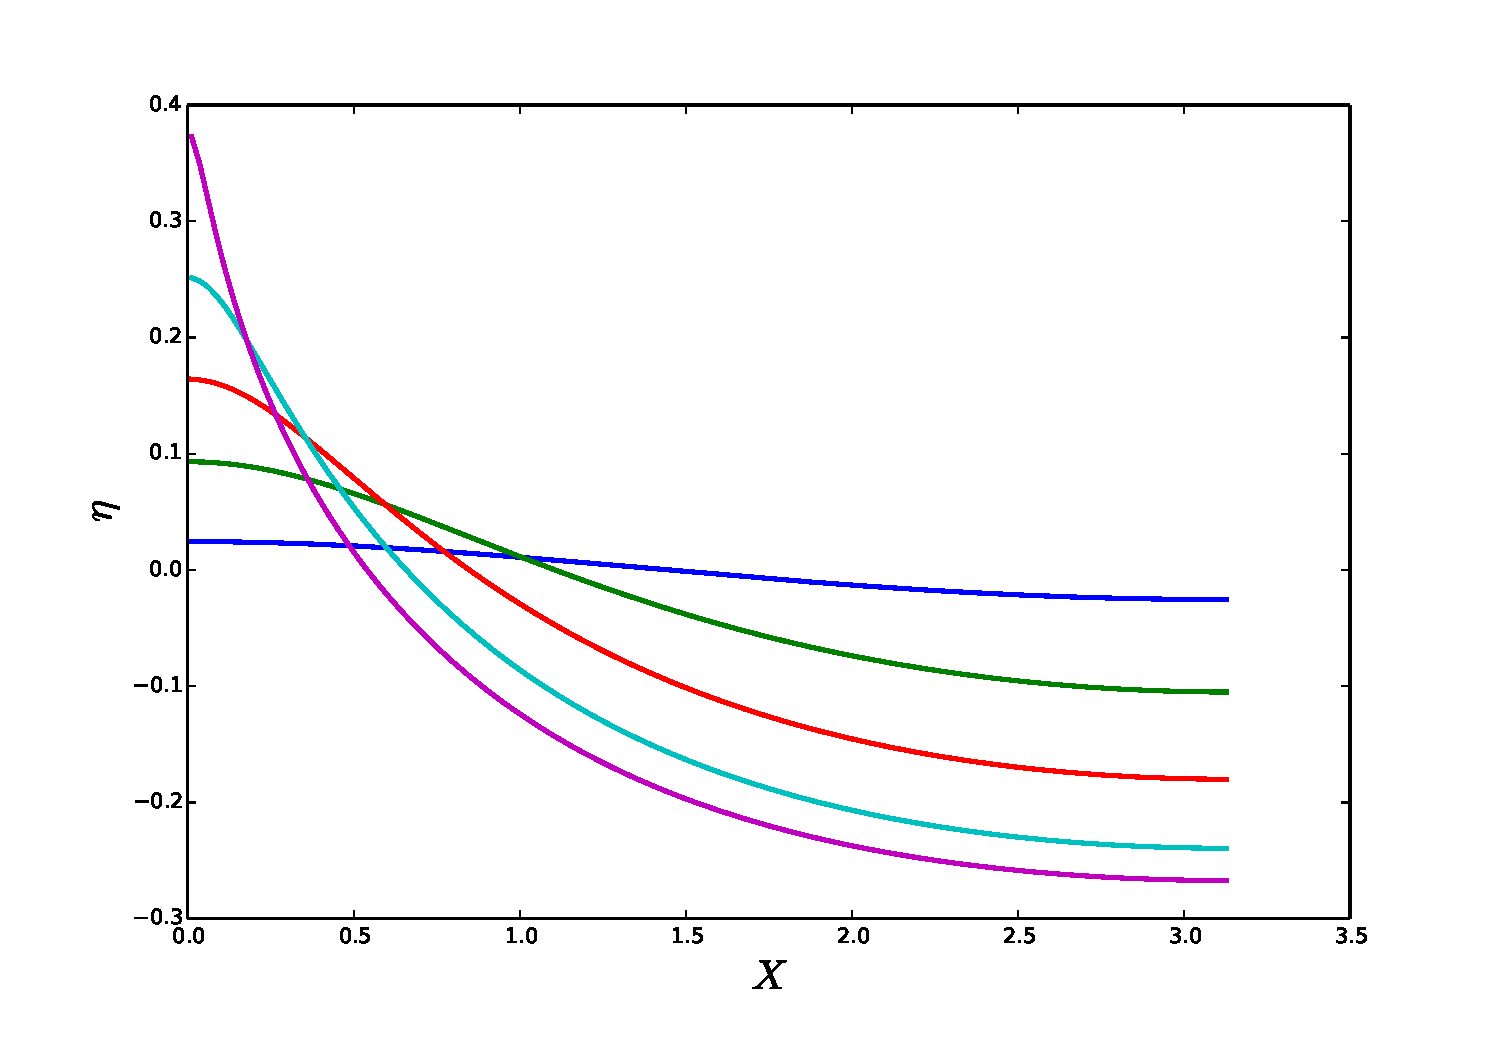
\includegraphics[scale=0.25]{Whitham_trav_solutions.pdf}
%		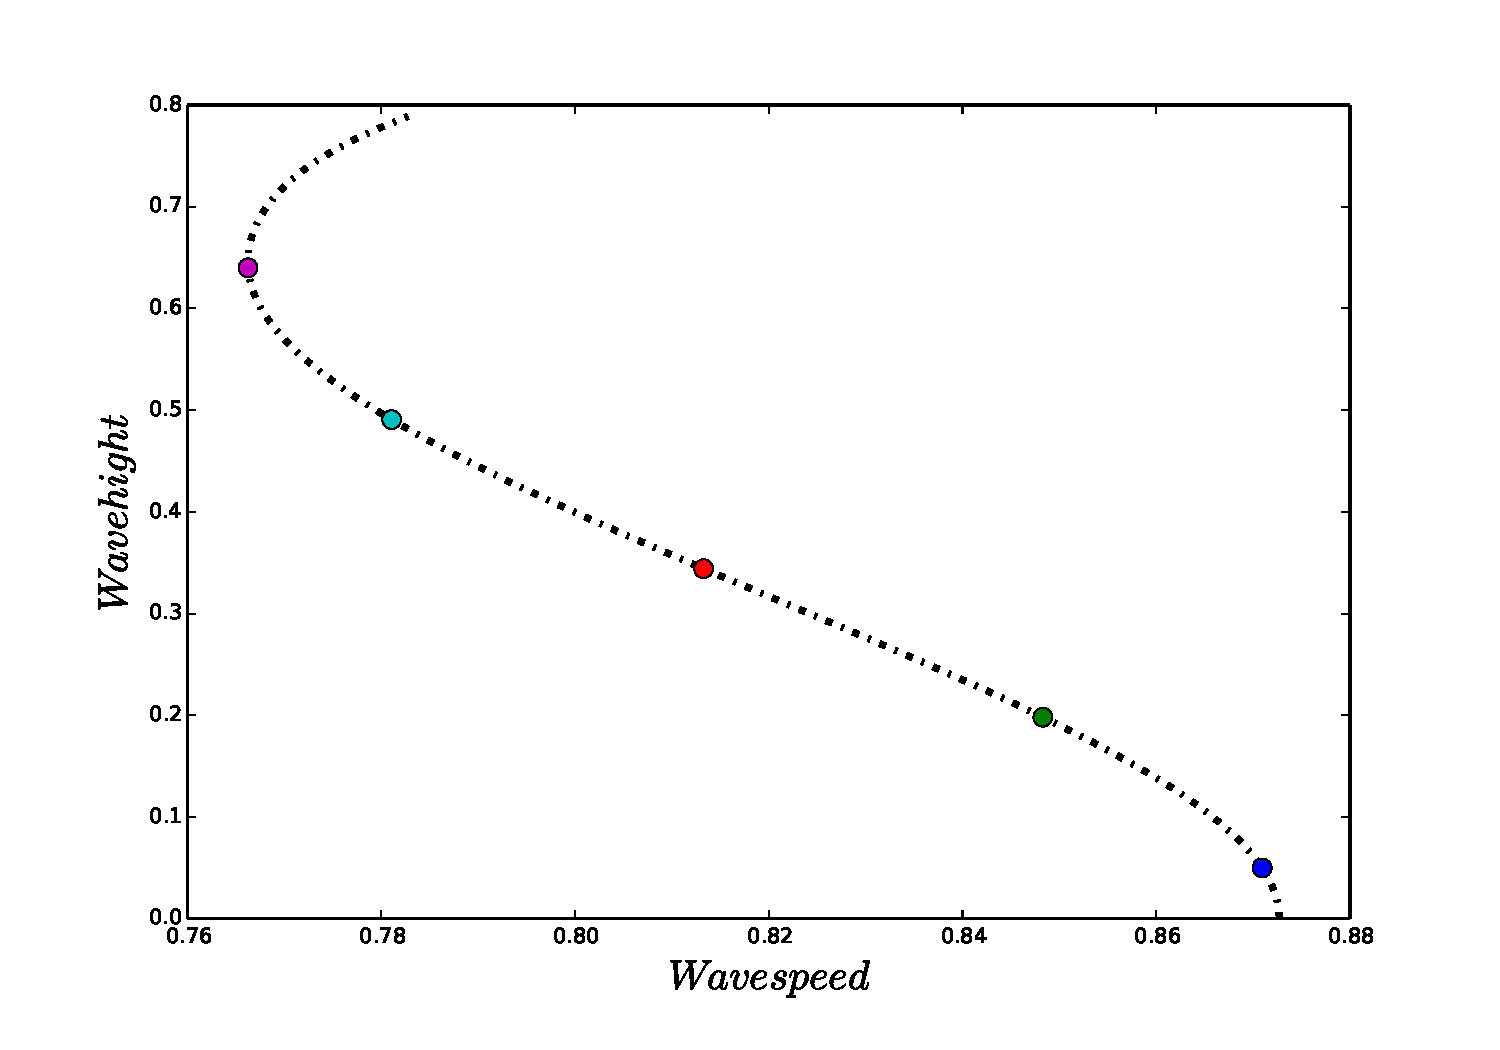
\includegraphics[scale=0.25]{Whitham_trav_bifur_curve.pdf}
%	\end{figure}
\end{frame}
%%%%%%%%%%%%%%%%%%%%%%%%%%%%%%%%%%%%%%%%%%%%%%%%%%%%%%%%%%%%%%%%%%%%%%%%%%%%%
%%%%---------------------------------------------------------------------%%%%
%%%%%%%%%%%%%%%%%%%%%%%%%%%%%%%%%%%%%%%%%%%%%%%%%%%%%%%%%%%%%%%%%%%%%%%%%%%%%

\subsection{Evolution test}
%%%%%%%%%%%%%%%%%%%%%%%%%%%%%%%%%%%%%%%%%%%%%%%%%%%%%%%%%%%%%%%%%%%%%%%%%%%%%
%%%%---------------------------------------------------------------------%%%%
%%%%%%%%%%%%%%%%%%%%%%%%%%%%%%%%%%%%%%%%%%%%%%%%%%%%%%%%%%%%%%%%%%%%%%%%%%%%%
\begin{frame}[t]{Evolution Test}
\onslide<1-2>{After a solution $\phi_N$ is found it can be tested with an evolution integrator, e.g. the 4th-order scheme given by De Frutos and Sanz-Serna (1992).}

\onslide<2-2>{ 
	
If the test is passed, the solution is recognized as stable. 	
%	\begin{figure}
%    	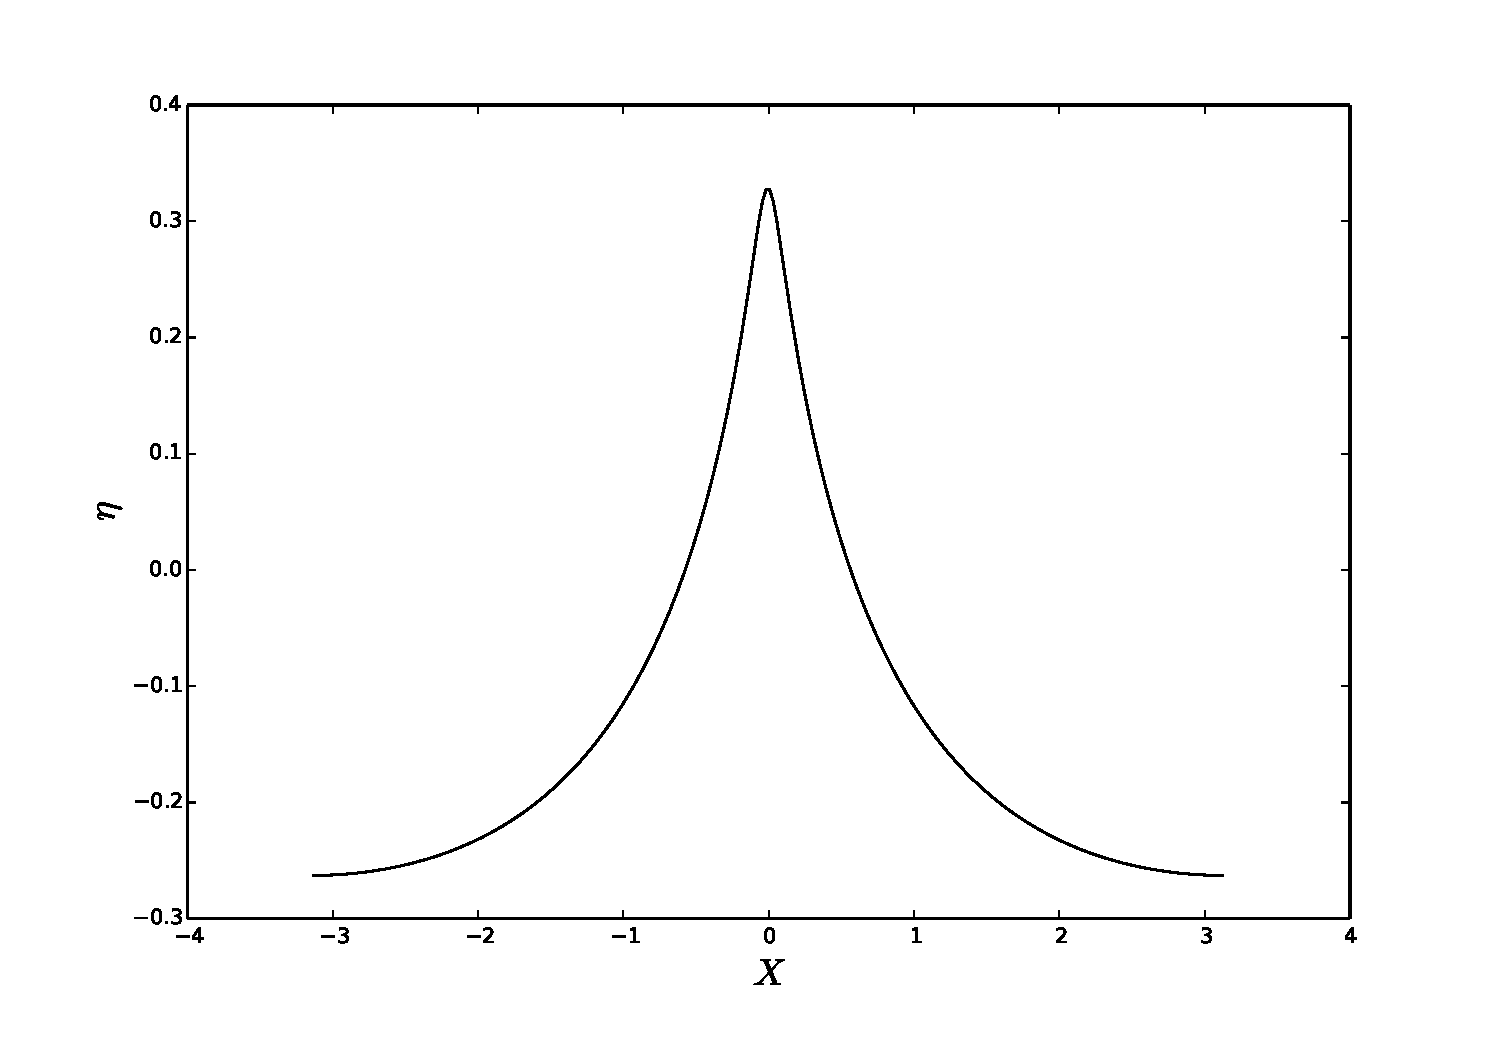
\includegraphics[scale=0.17]{Whitham_evtest_1.pdf}
%      	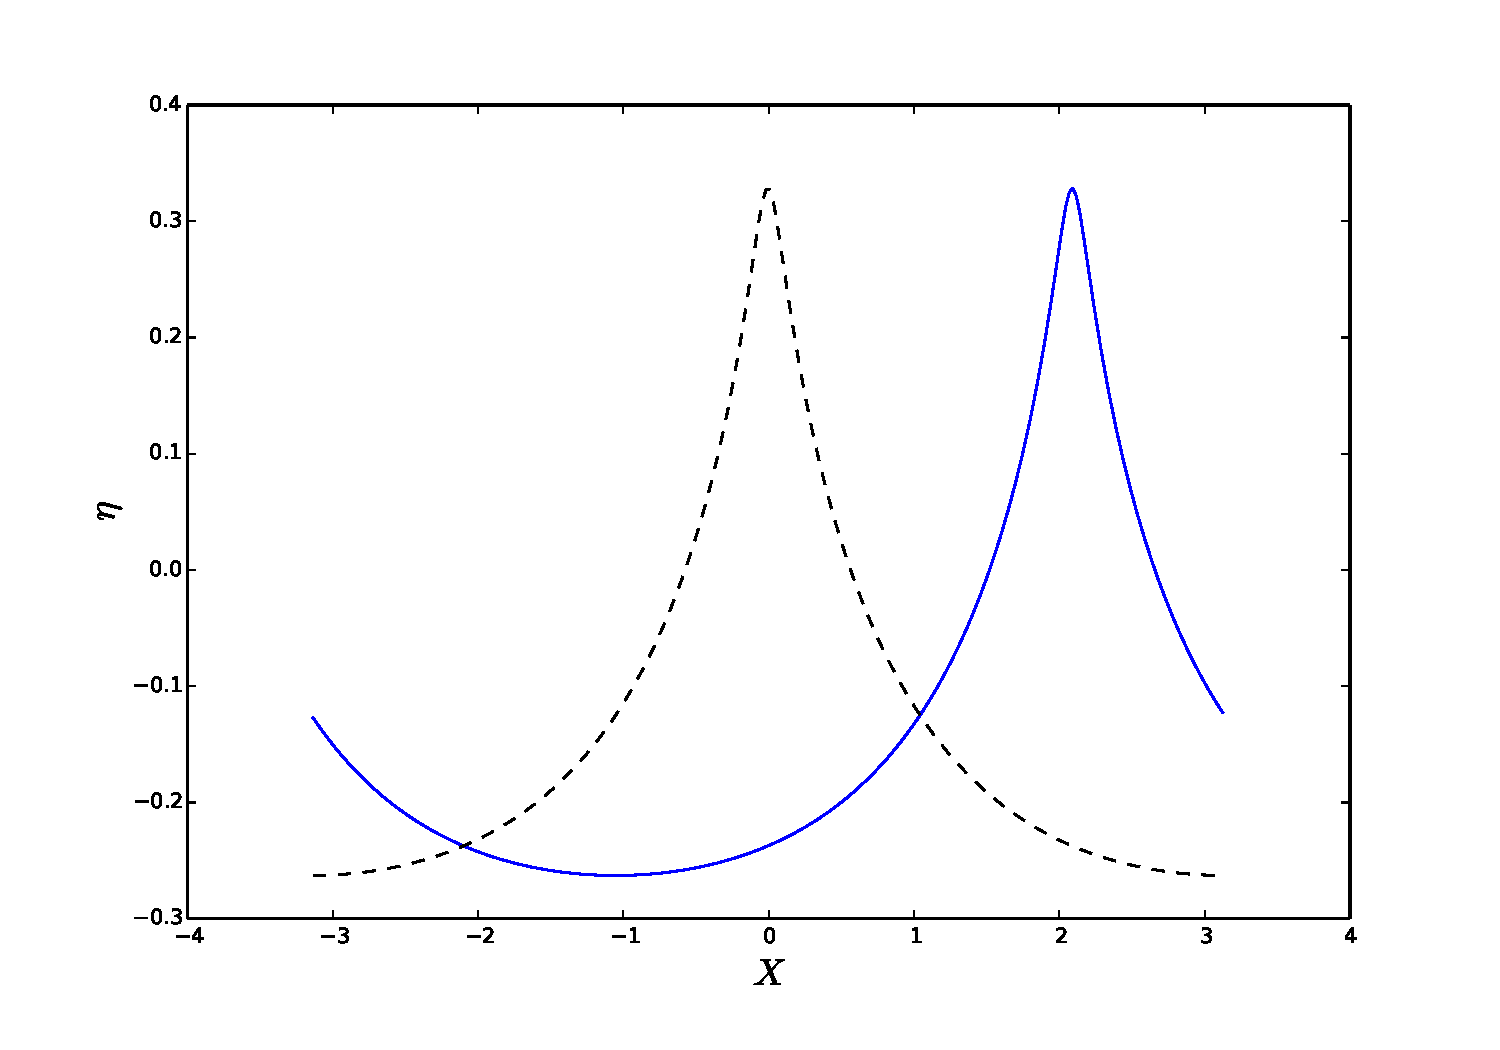
\includegraphics[scale=0.17]{Whitham_evtest_2.pdf}
%
%      	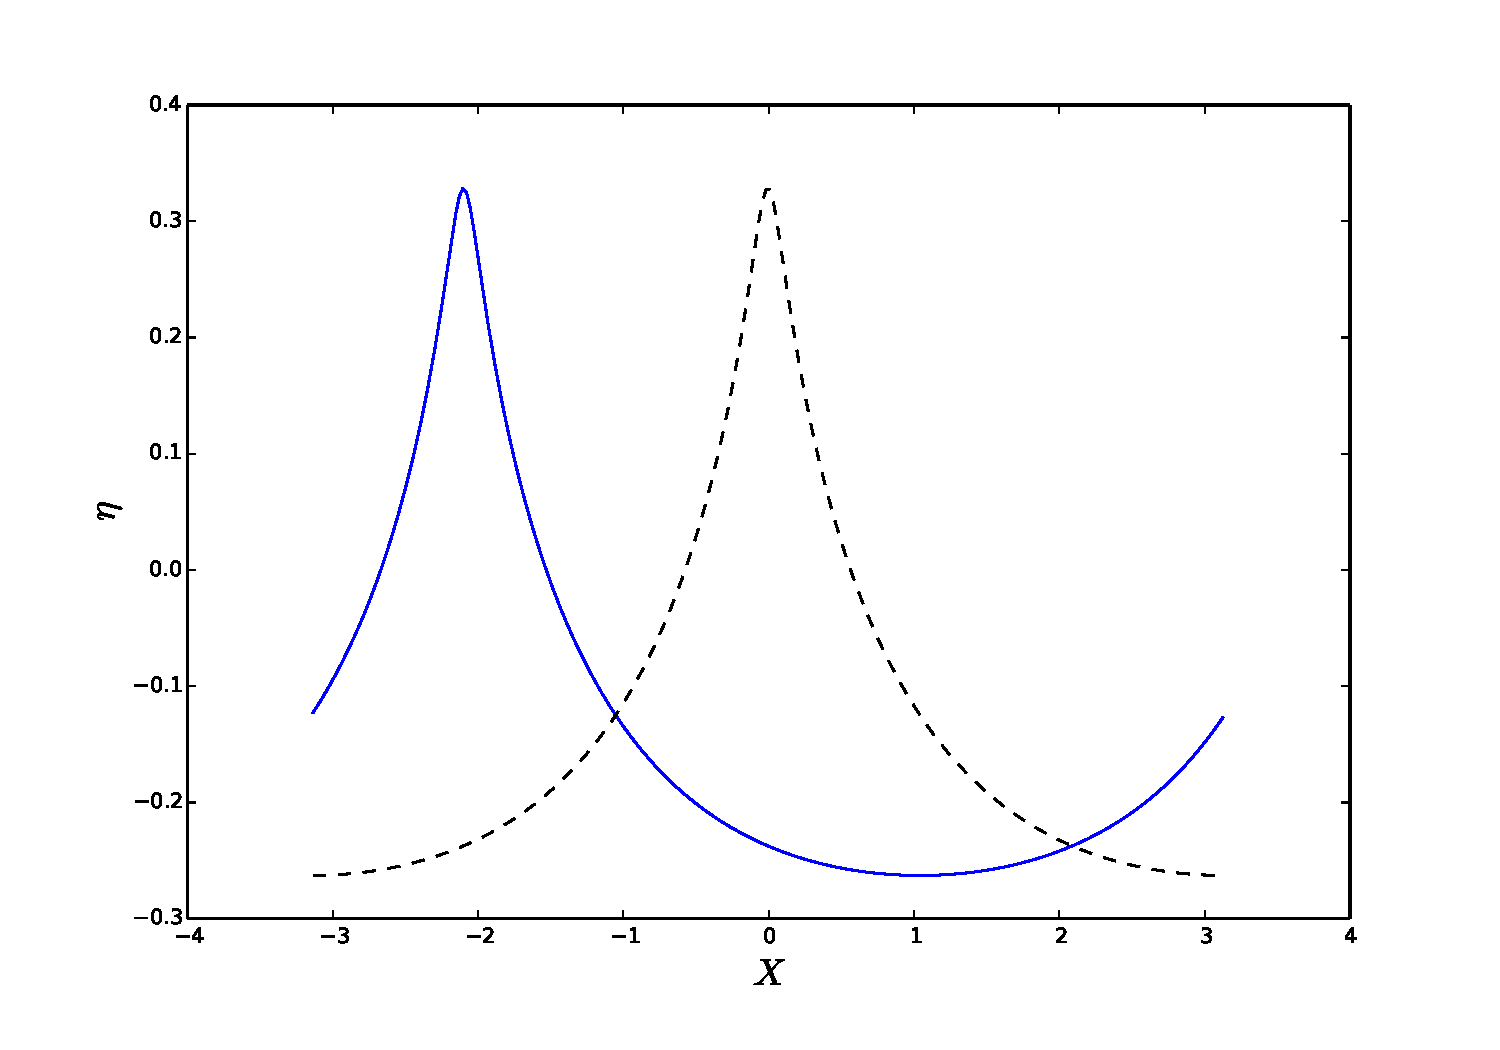
\includegraphics[scale=0.17]{Whitham_evtest_3.pdf}
%      	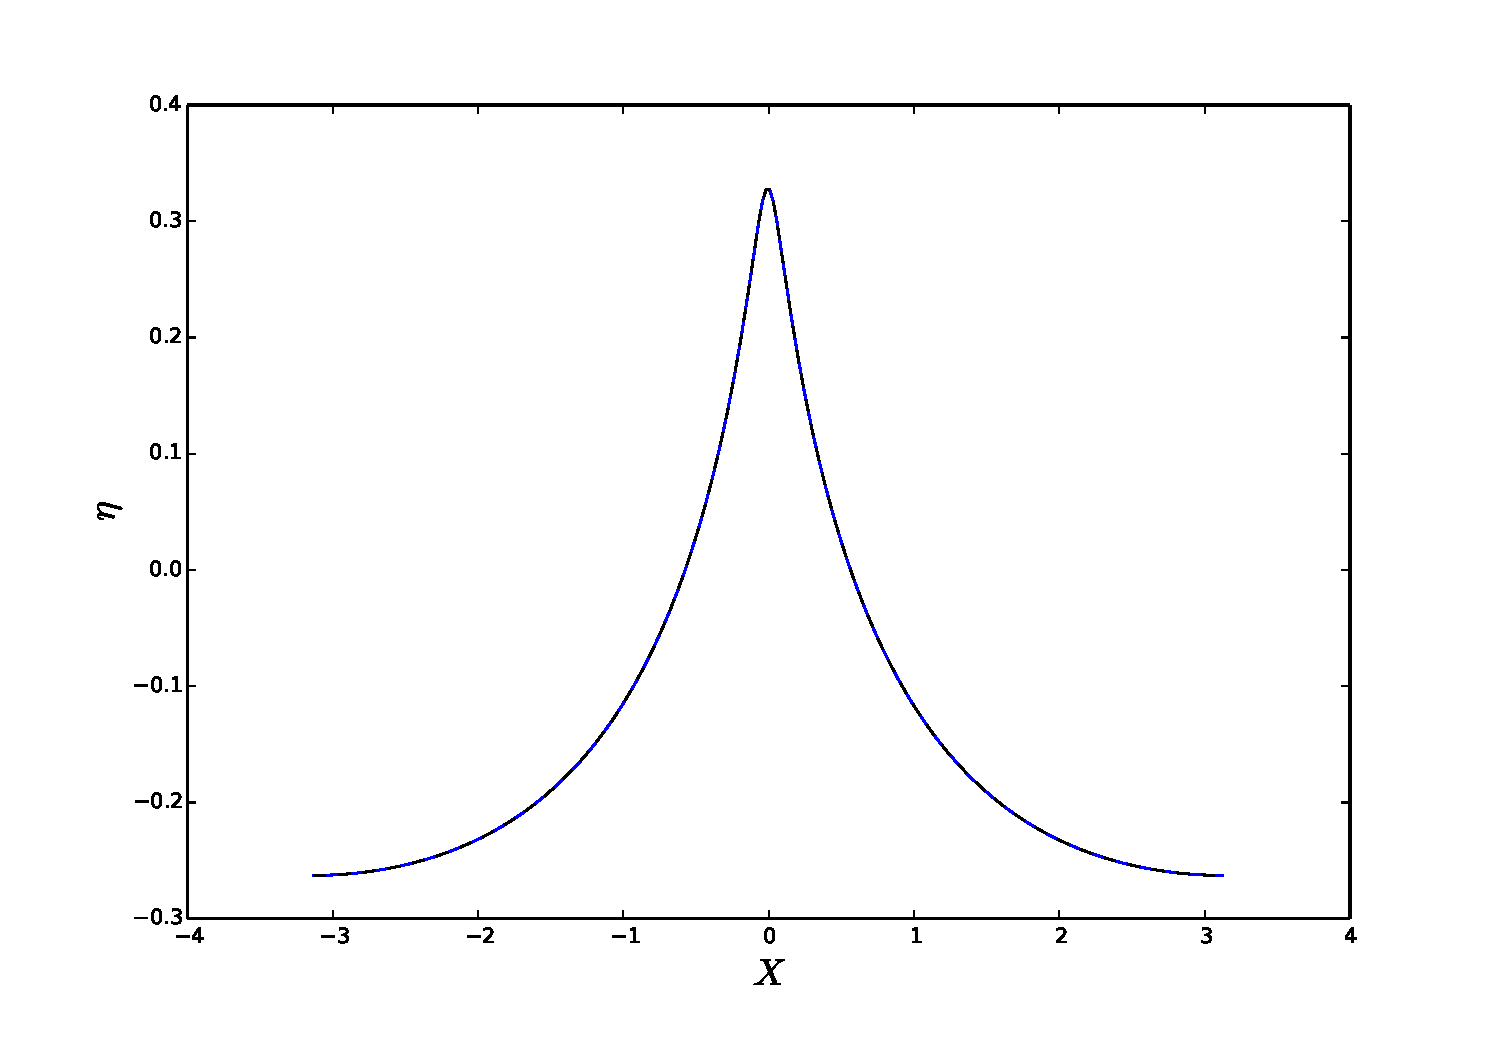
\includegraphics[scale=0.17]{Whitham_evtest_4.pdf}
%	\end{figure}
}
\end{frame}
%%%%%%%%%%%%%%%%%%%%%%%%%%%%%%%%%%%%%%%%%%%%%%%%%%%%%%%%%%%%%%%%%%%%%%%%%%%%%
%%%%---------------------------------------------------------------------%%%%
%%%%%%%%%%%%%%%%%%%%%%%%%%%%%%%%%%%%%%%%%%%%%%%%%%%%%%%%%%%%%%%%%%%%%%%%%%%%%

\section{Python-based Solver Package}
\subsection{Advantages of Python}
%%%%%%%%%%%%%%%%%%%%%%%%%%%%%%%%%%%%%%%%%%%%%%%%%%%%%%%%%%%%%%%%%%%%%%%%%%%%%
%%%%---------------------------------------------------------------------%%%%
%%%%%%%%%%%%%%%%%%%%%%%%%%%%%%%%%%%%%%%%%%%%%%%%%%%%%%%%%%%%%%%%%%%%%%%%%%%%%
\begin{frame}[t]{Advantages of Python}
Python - high level programming language.
	\begin{itemize}
	\item support of multiple paradigms: \textcolor{blue}{object-oriented}, imperative and functional 

	\item often used as a scripting language

	\item different libraries, handy features and tools 

	\item a large helpful community

	\item advantage over some other products - \textcolor{blue}{\textbf{IT is FREE}}
	\end{itemize}
%	\begin{figure}
%		\centering
%		
\includegraphics[scale=0.5]{python-logo.pdf}
%	\end{figure}
\end{frame}
%%%%%%%%%%%%%%%%%%%%%%%%%%%%%%%%%%%%%%%%%%%%%%%%%%%%%%%%%%%%%%%%%%%%%%%%%%%%%
%%%%---------------------------------------------------------------------%%%%
%%%%%%%%%%%%%%%%%%%%%%%%%%%%%%%%%%%%%%%%%%%%%%%%%%%%%%%%%%%%%%%%%%%%%%%%%%%%%

\section{Stability of solutions}
\subsection{Whitham equation}
%%%%%%%%%%%%%%%%%%%%%%%%%%%%%%%%%%%%%%%%%%%%%%%%%%%%%%%%%%%%%%%%%%%%%%%%%%%%%
%%%%---------------------------------------------------------------------%%%%
%%%%%%%%%%%%%%%%%%%%%%%%%%%%%%%%%%%%%%%%%%%%%%%%%%%%%%%%%%%%%%%%%%%%%%%%%%%%%
\begin{frame}[t]{Stability of solutions: Whitham equation}

\centering{Whitham bifurcation curve ($\mbox{wavelength} = 2 \pi$). }

%	\begin{figure}[htbp]    
%		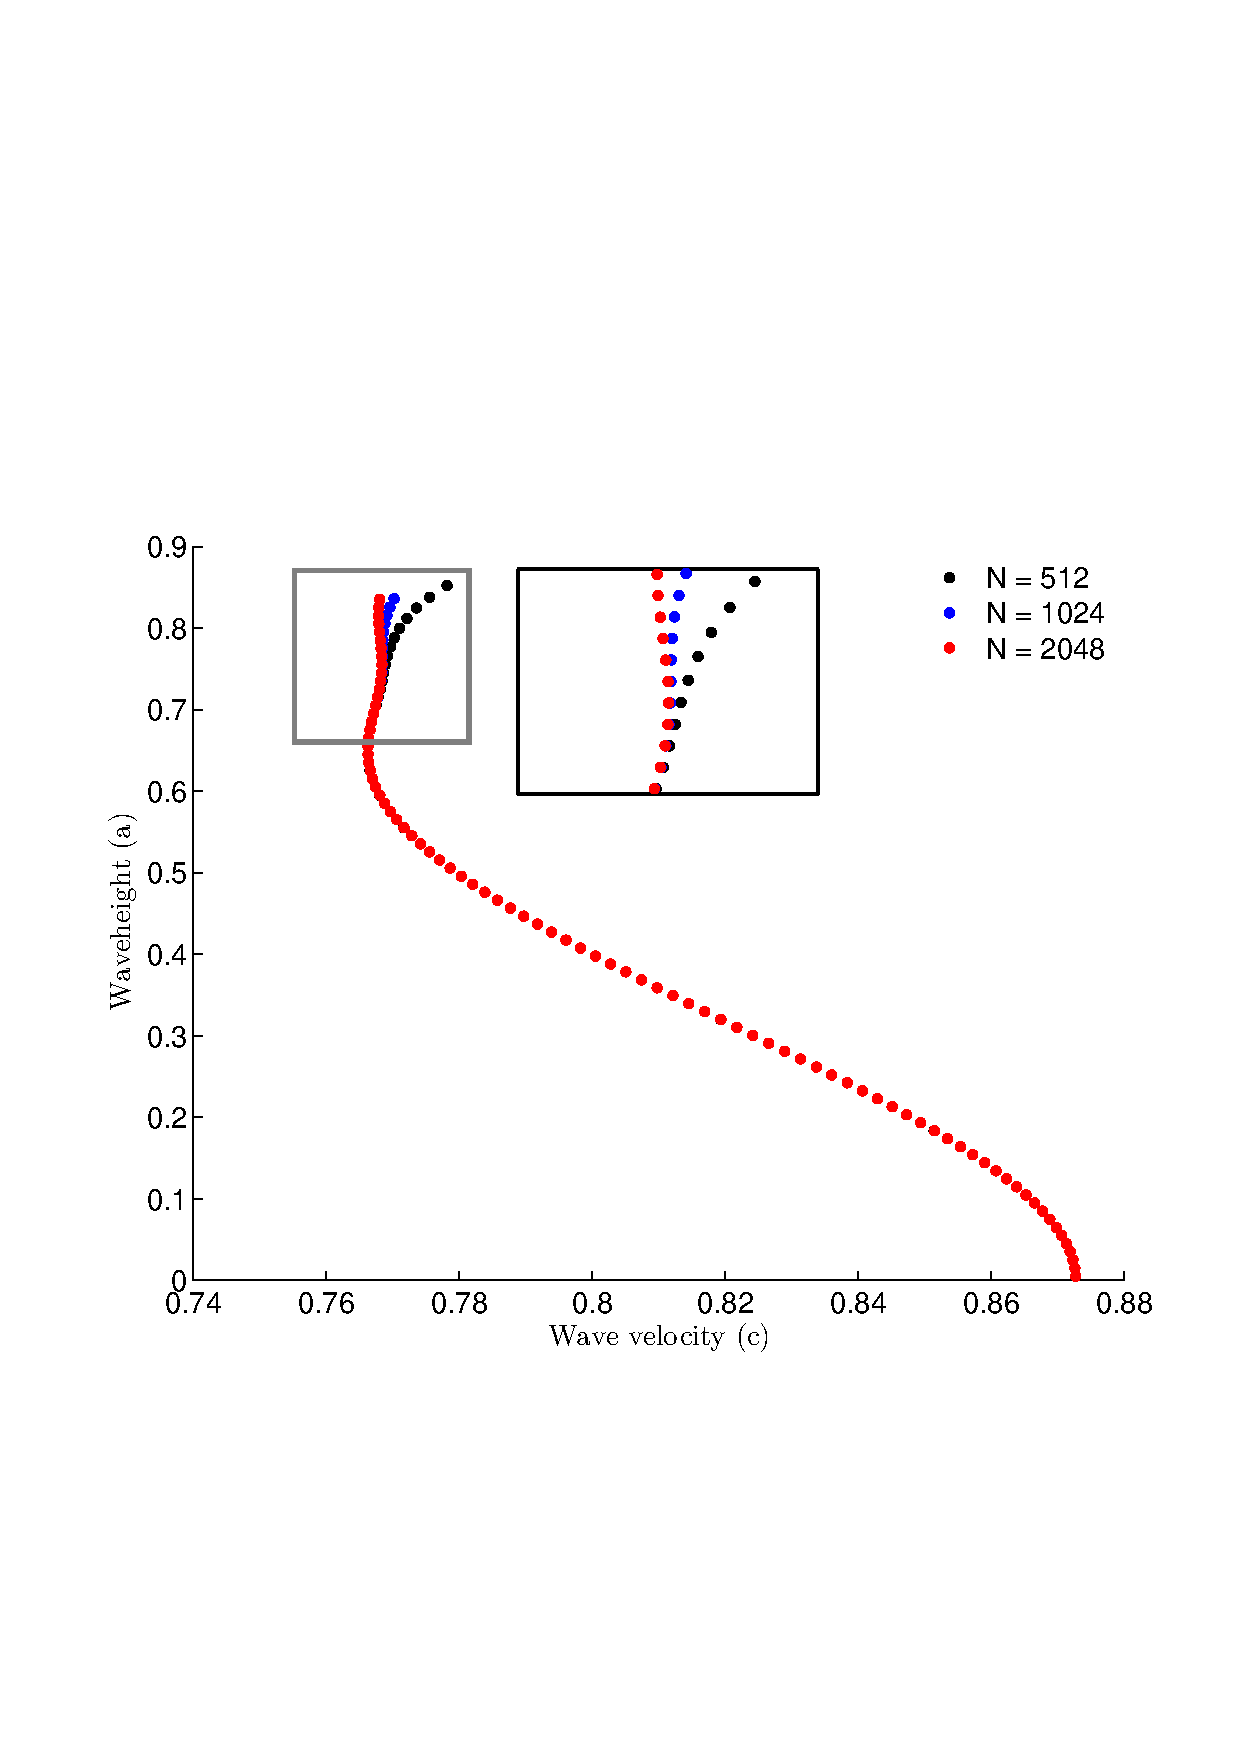
\includegraphics[scale=0.47, trim = 1.2cm 6.5cm 0.6cm 8cm, clip]{512_1024_2048.pdf}
%	\end{figure}
\end{frame}
%%%%%%%%%%%%%%%%%%%%%%%%%%%%%%%%%%%%%%%%%%%%%%%%%%%%%%%%%%%%%%%%%%%%%%%%%%%%%
%%%%---------------------------------------------------------------------%%%%
%%%%%%%%%%%%%%%%%%%%%%%%%%%%%%%%%%%%%%%%%%%%%%%%%%%%%%%%%%%%%%%%%%%%%%%%%%%%%
\begin{frame}[t]{Stability of solutions: Whitham equation}

\centering{Whitham bifurcation curve ($\mbox{wavelength} = 2 \pi$). }

\begin{align*}
V( \phi_c ) &= \frac{1}{2} \int_{-\infty}^{+\infty} \phi_c ^2~d\zeta, \qquad~~
E( \phi_c ) = \frac{1}{2}\int_{-\infty}^{+\infty} \frac{1}{2} \phi_c ^3 + K \phi_c ^2~d\zeta.\\
d(c) &= E( \phi_c ) -c V( \phi_c ), \qquad d'(c)=V( \phi_c )= 1/2\|\phi_c\|_{L^2}^2.
\end{align*}

%	\begin{figure}[htbp]    
%		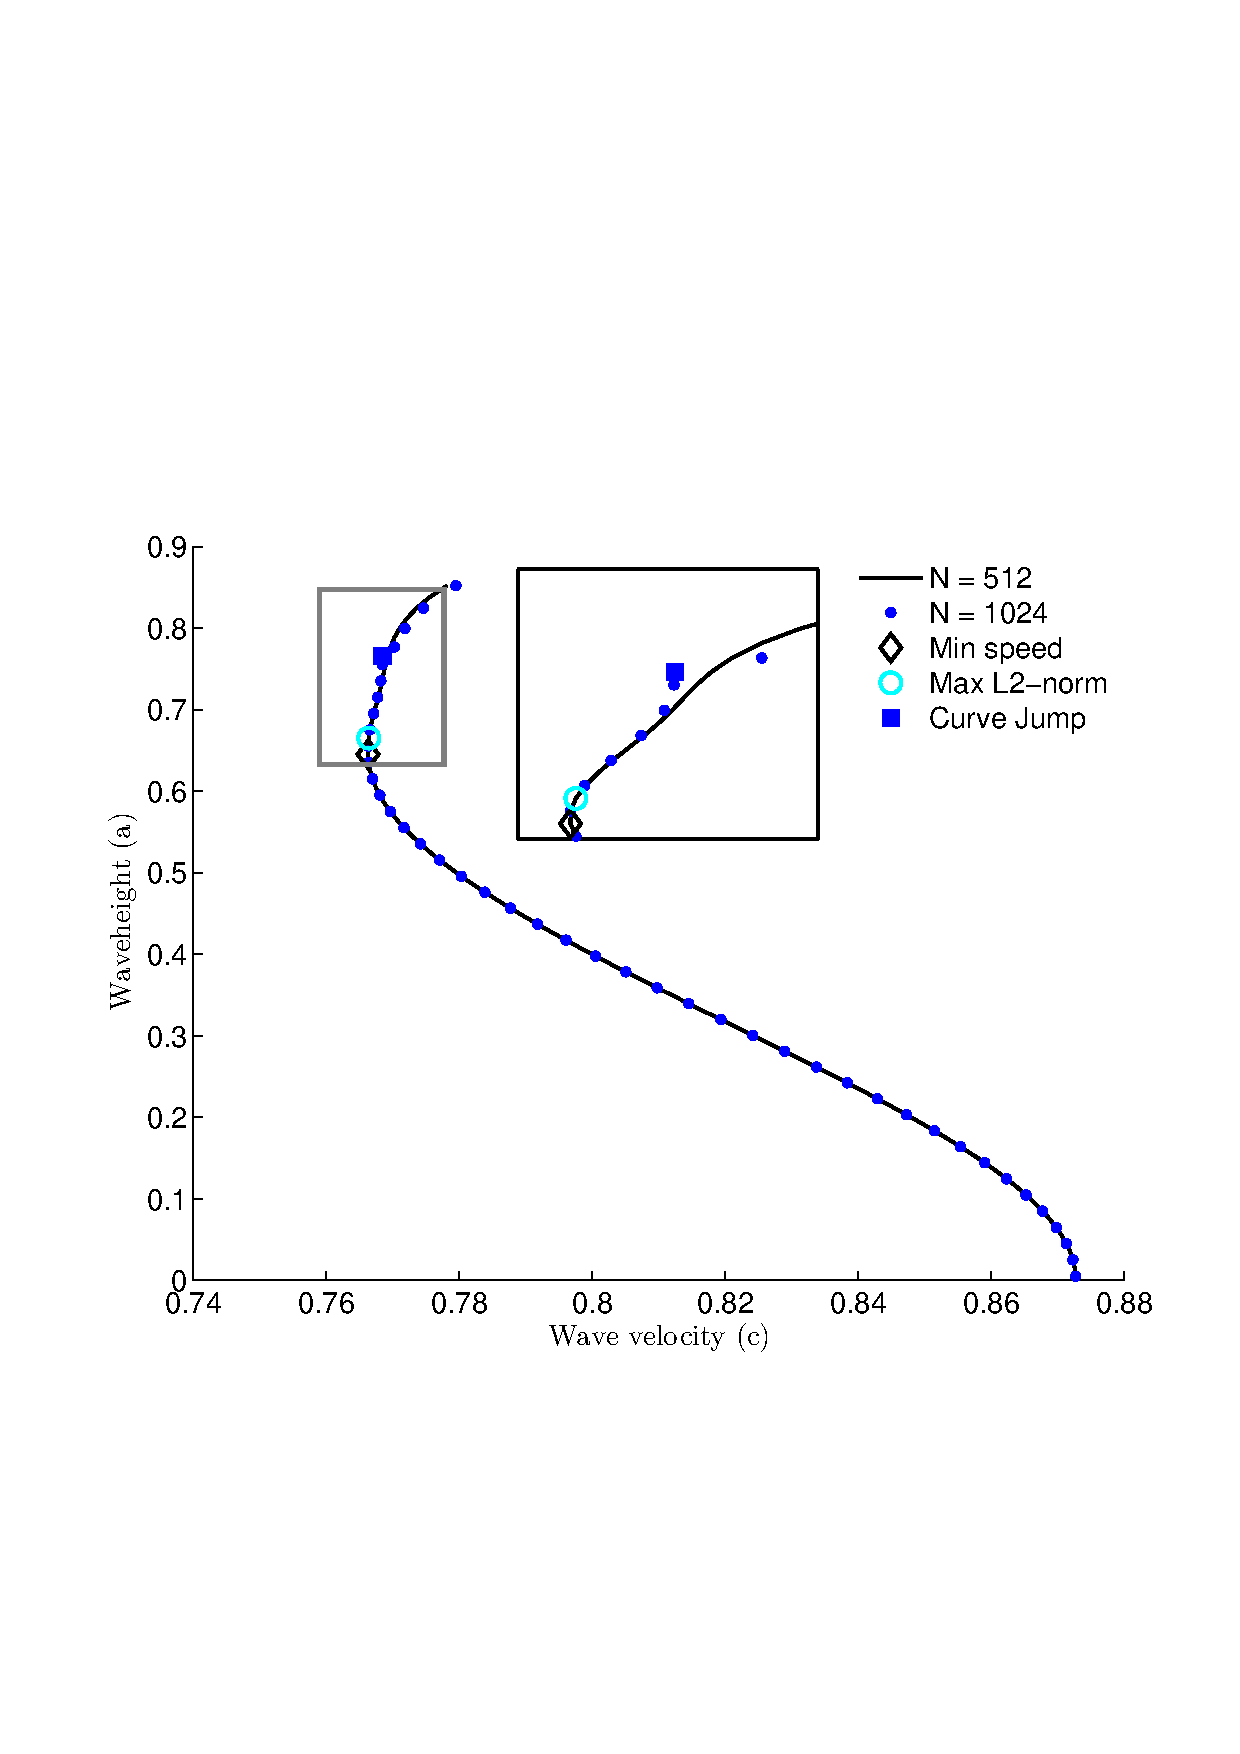
\includegraphics[scale=0.31, trim = 1.2cm 6.5cm 0.6cm 8cm, clip]{512_1024.pdf}
%		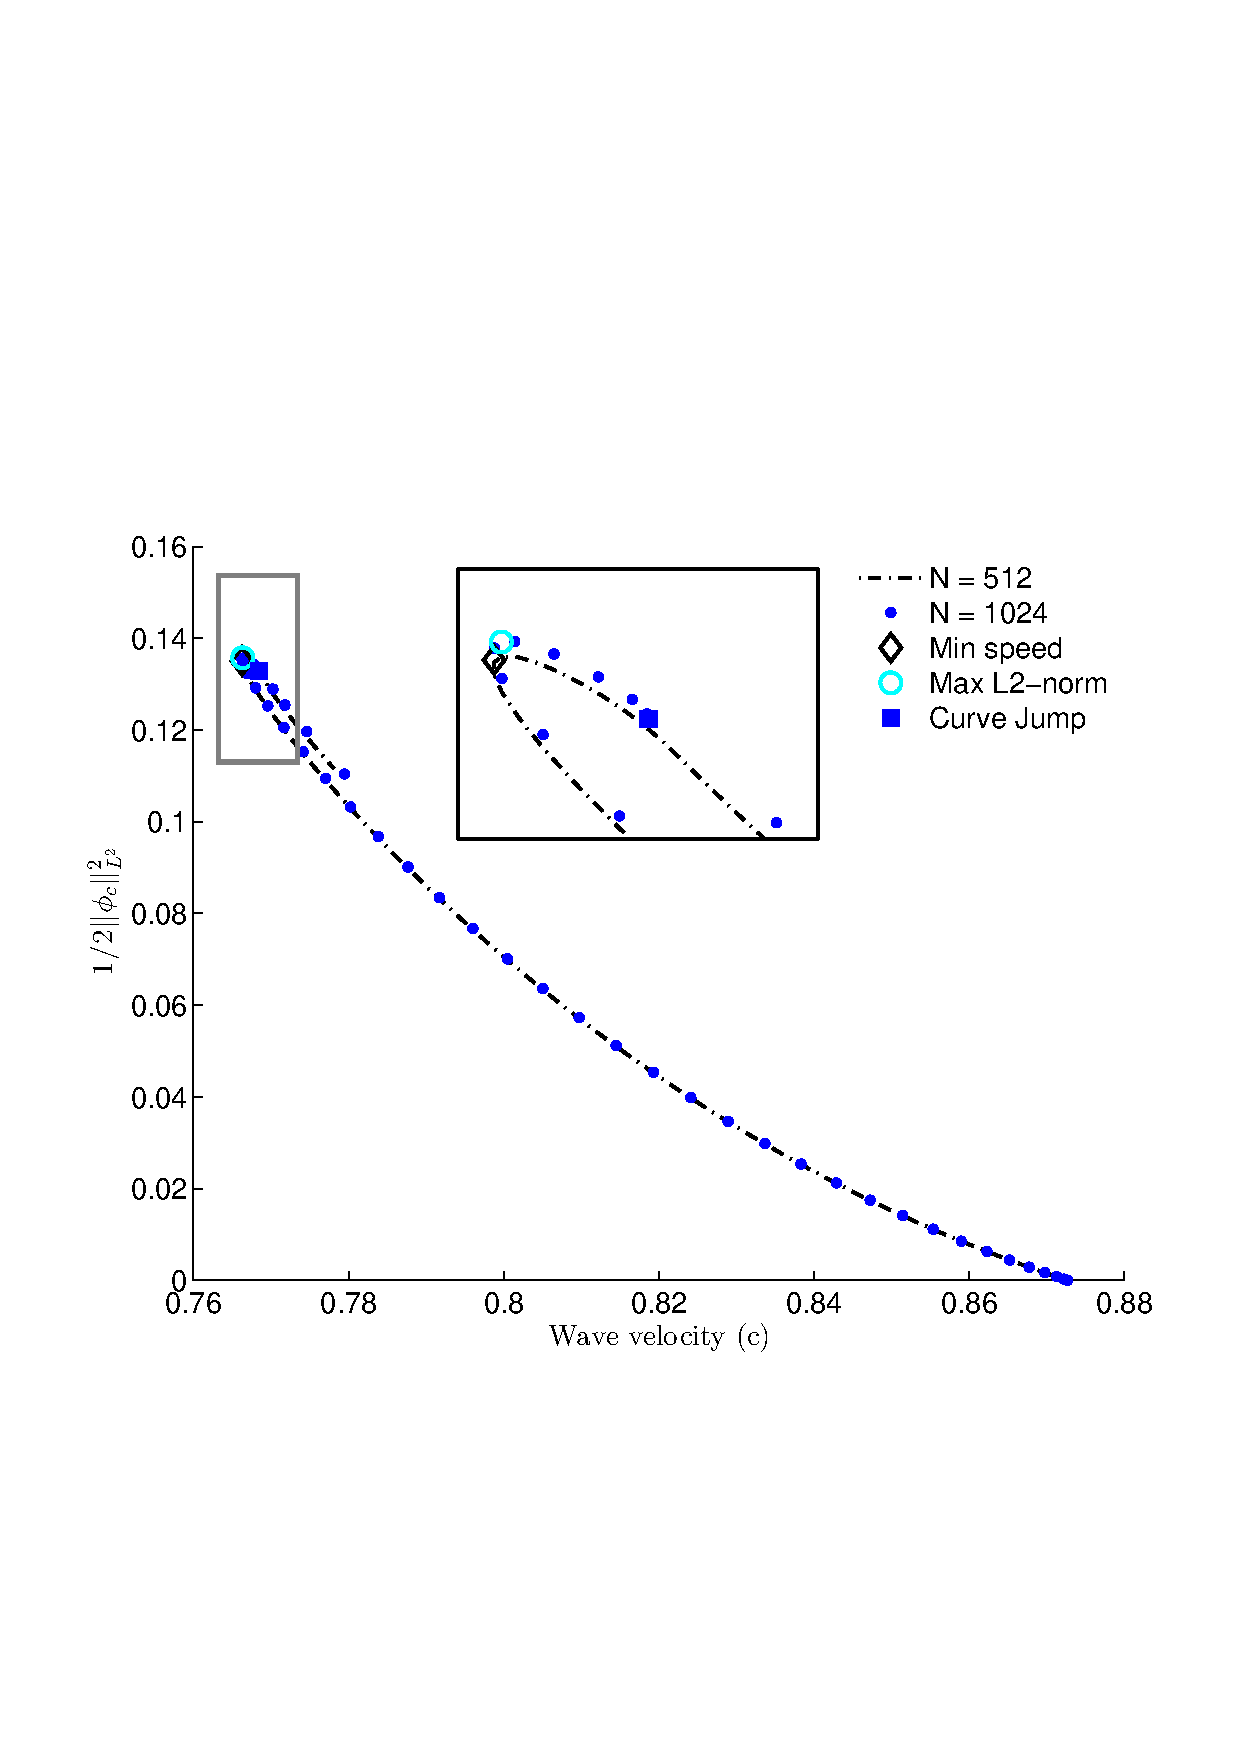
\includegraphics[scale=0.31, trim = 1.2cm 6.5cm 0.6cm 8cm, clip]{L2_512_1024.pdf}
%	\end{figure}
\end{frame}
%%%%%%%%%%%%%%%%%%%%%%%%%%%%%%%%%%%%%%%%%%%%%%%%%%%%%%%%%%%%%%%%%%%%%%%%%%%%%
%%%%---------------------------------------------------------------------%%%%
%%%%%%%%%%%%%%%%%%%%%%%%%%%%%%%%%%%%%%%%%%%%%%%%%%%%%%%%%%%%%%%%%%%%%%%%%%%%%
\begin{frame}[t]{Stability of solutions: Whitham equation}
\centering{Whitham bifurcation curve ($\mbox{wavelength} = 2 \pi$). }
%	\begin{figure}[htbp]    
%		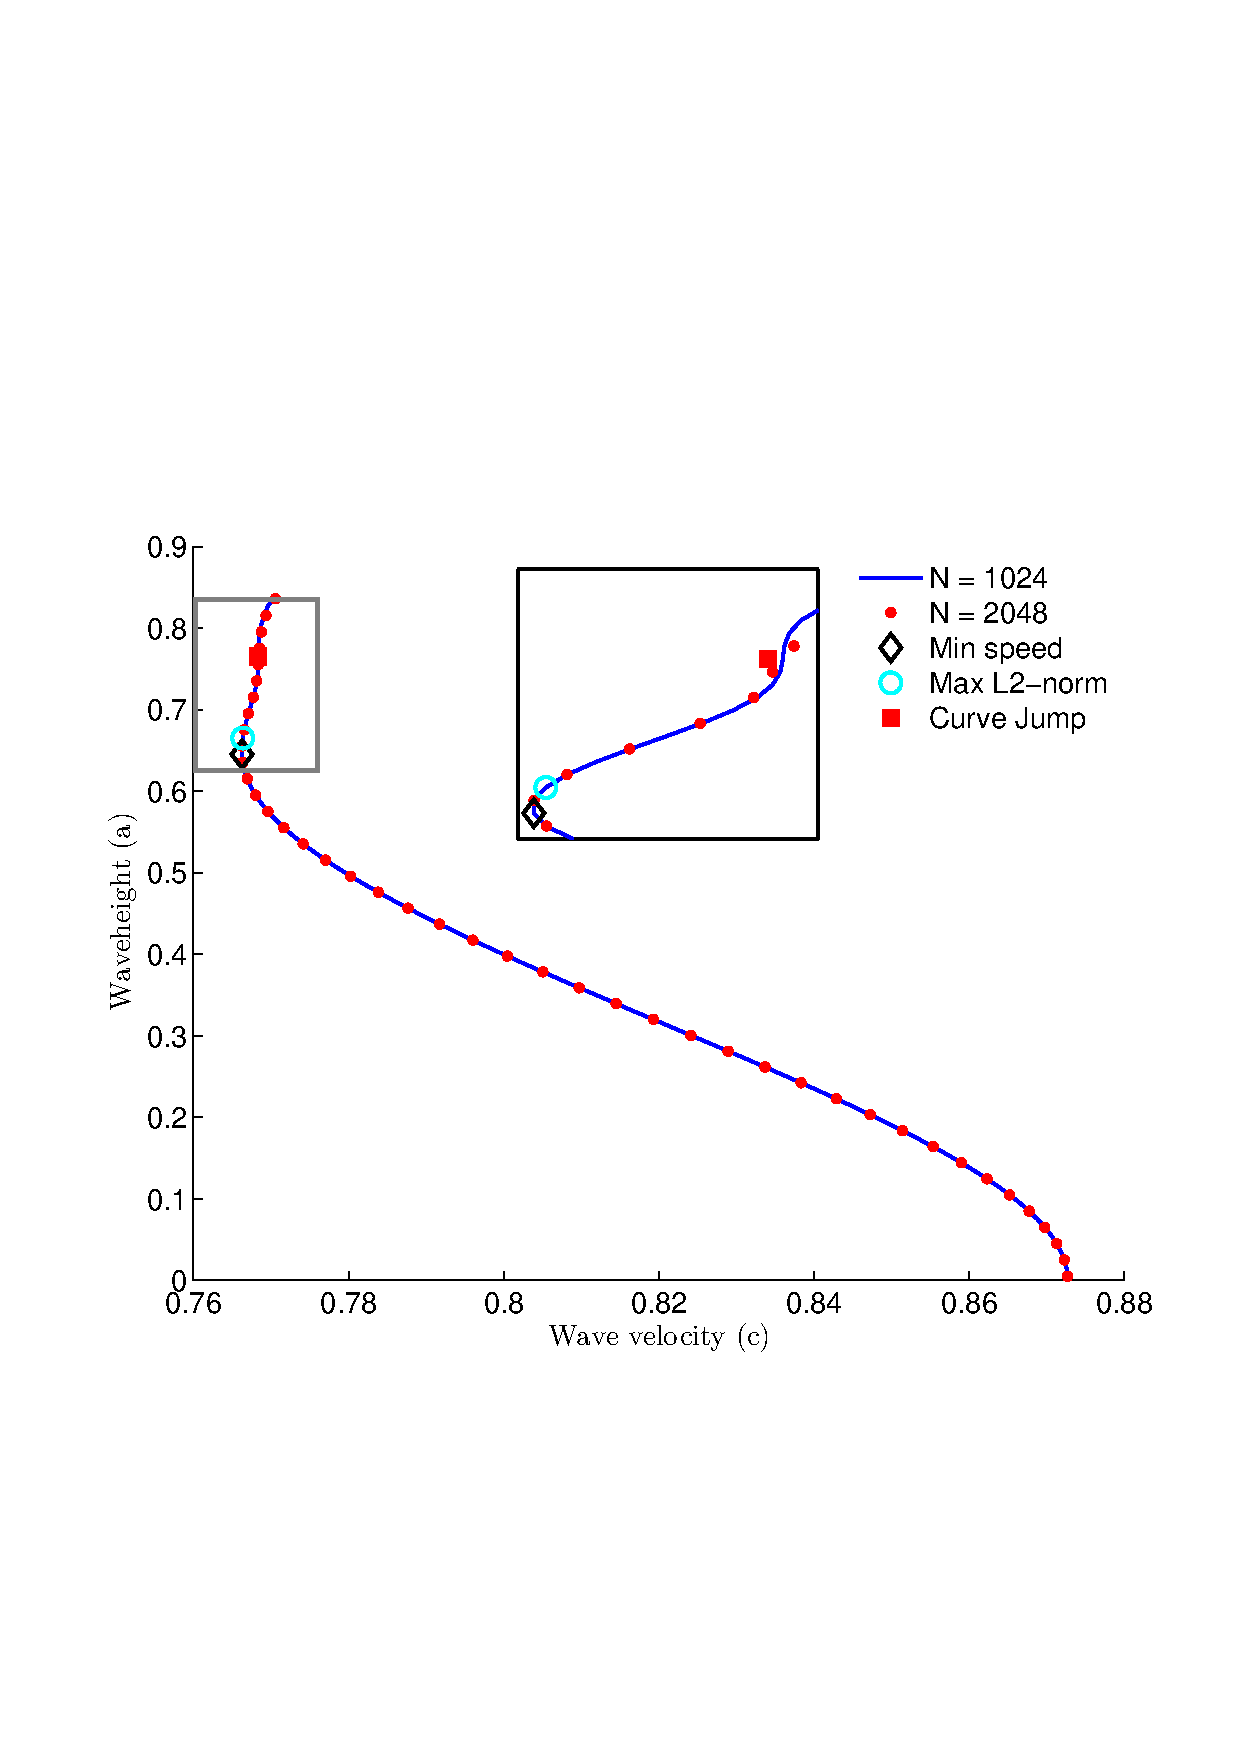
\includegraphics[scale=0.32, trim = 1.2cm 6.5cm 0.6cm 8cm, clip]{1024_2048.pdf}
%		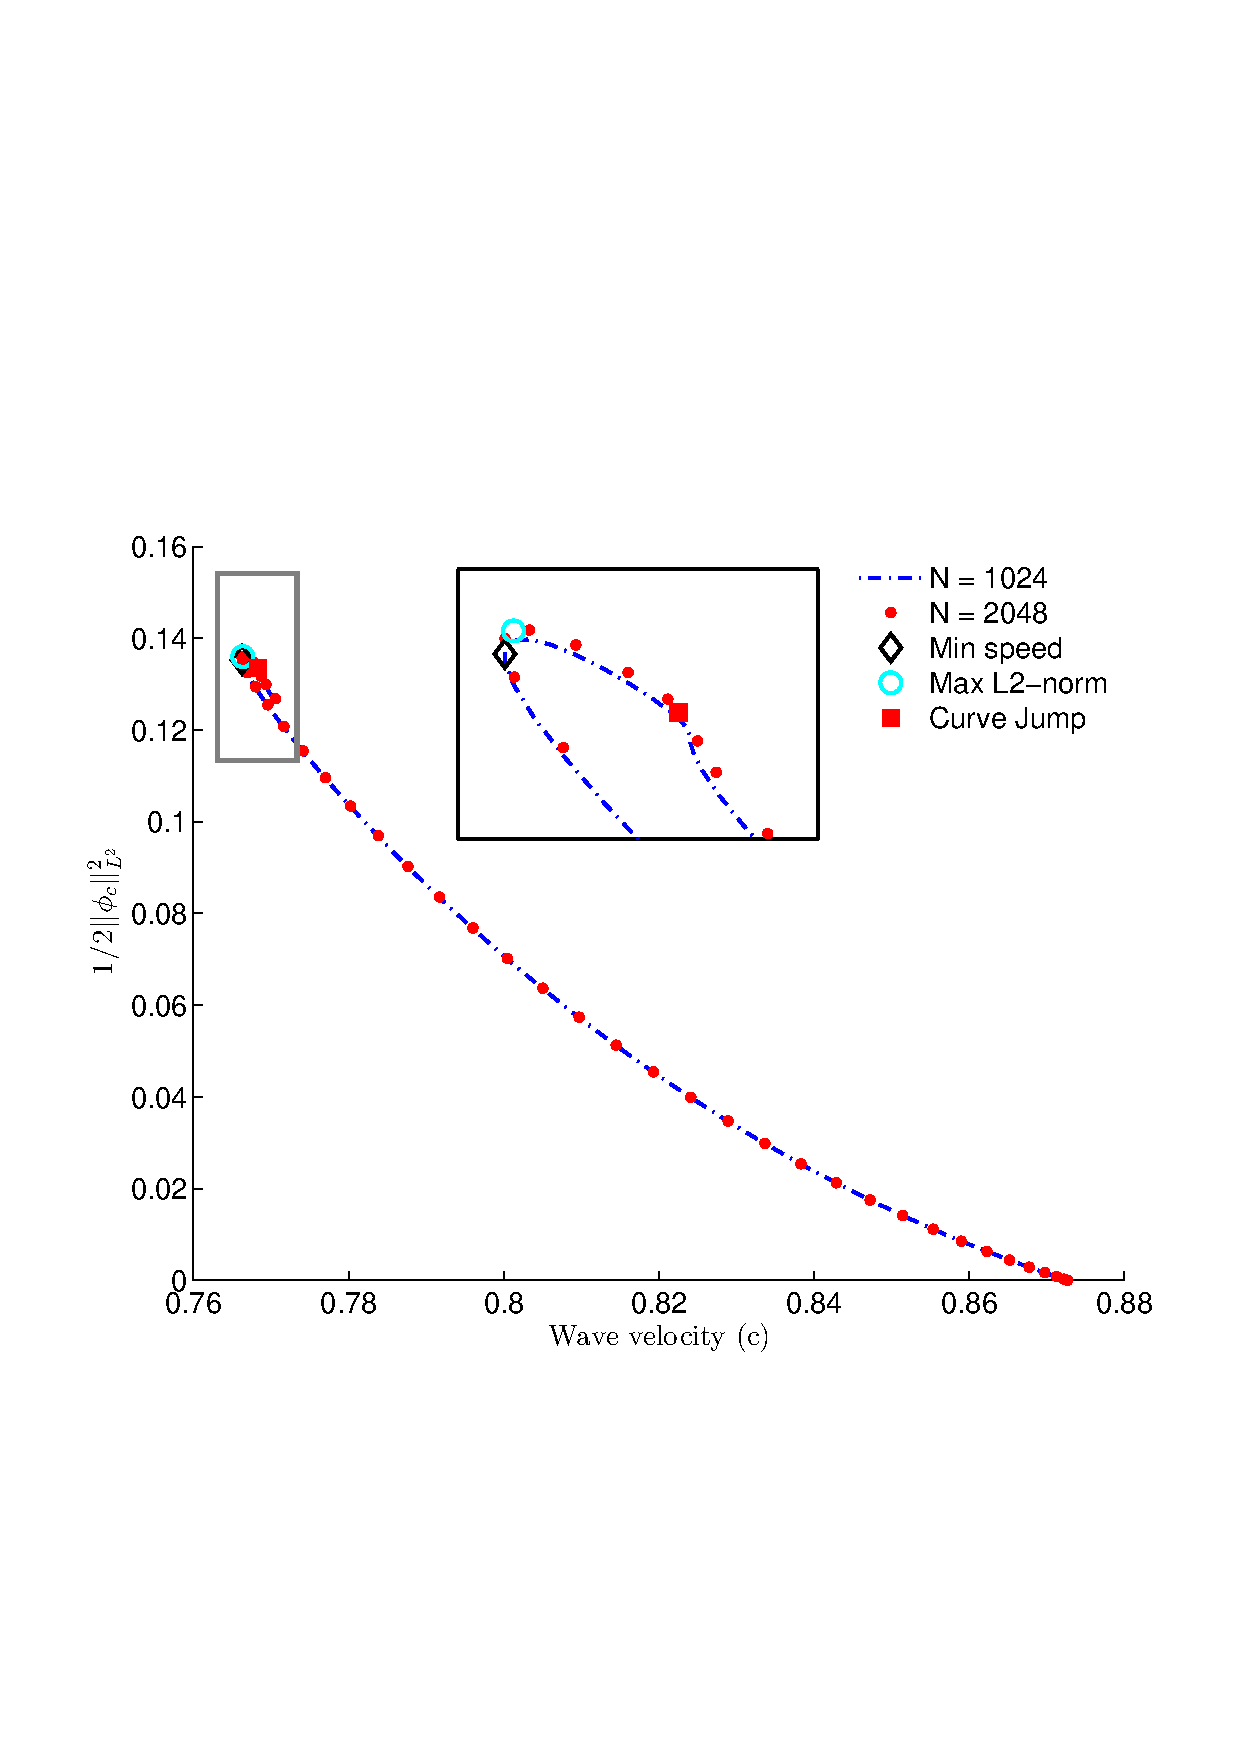
\includegraphics[scale=0.32, trim = 1.2cm 6.5cm 0.6cm 8cm, clip]{L2_1024_2048.pdf}
%	\end{figure}
\end{frame}
%%%%%%%%%%%%%%%%%%%%%%%%%%%%%%%%%%%%%%%%%%%%%%%%%%%%%%%%%%%%%%%%%%%%%%%%%%%%%
%%%%---------------------------------------------------------------------%%%%
%%%%%%%%%%%%%%%%%%%%%%%%%%%%%%%%%%%%%%%%%%%%%%%%%%%%%%%%%%%%%%%%%%%%%%%%%%%%%
\begin{frame}[t]{Stability of solutions: Whitham equation}
%	\begin{figure}[htbp]    
%		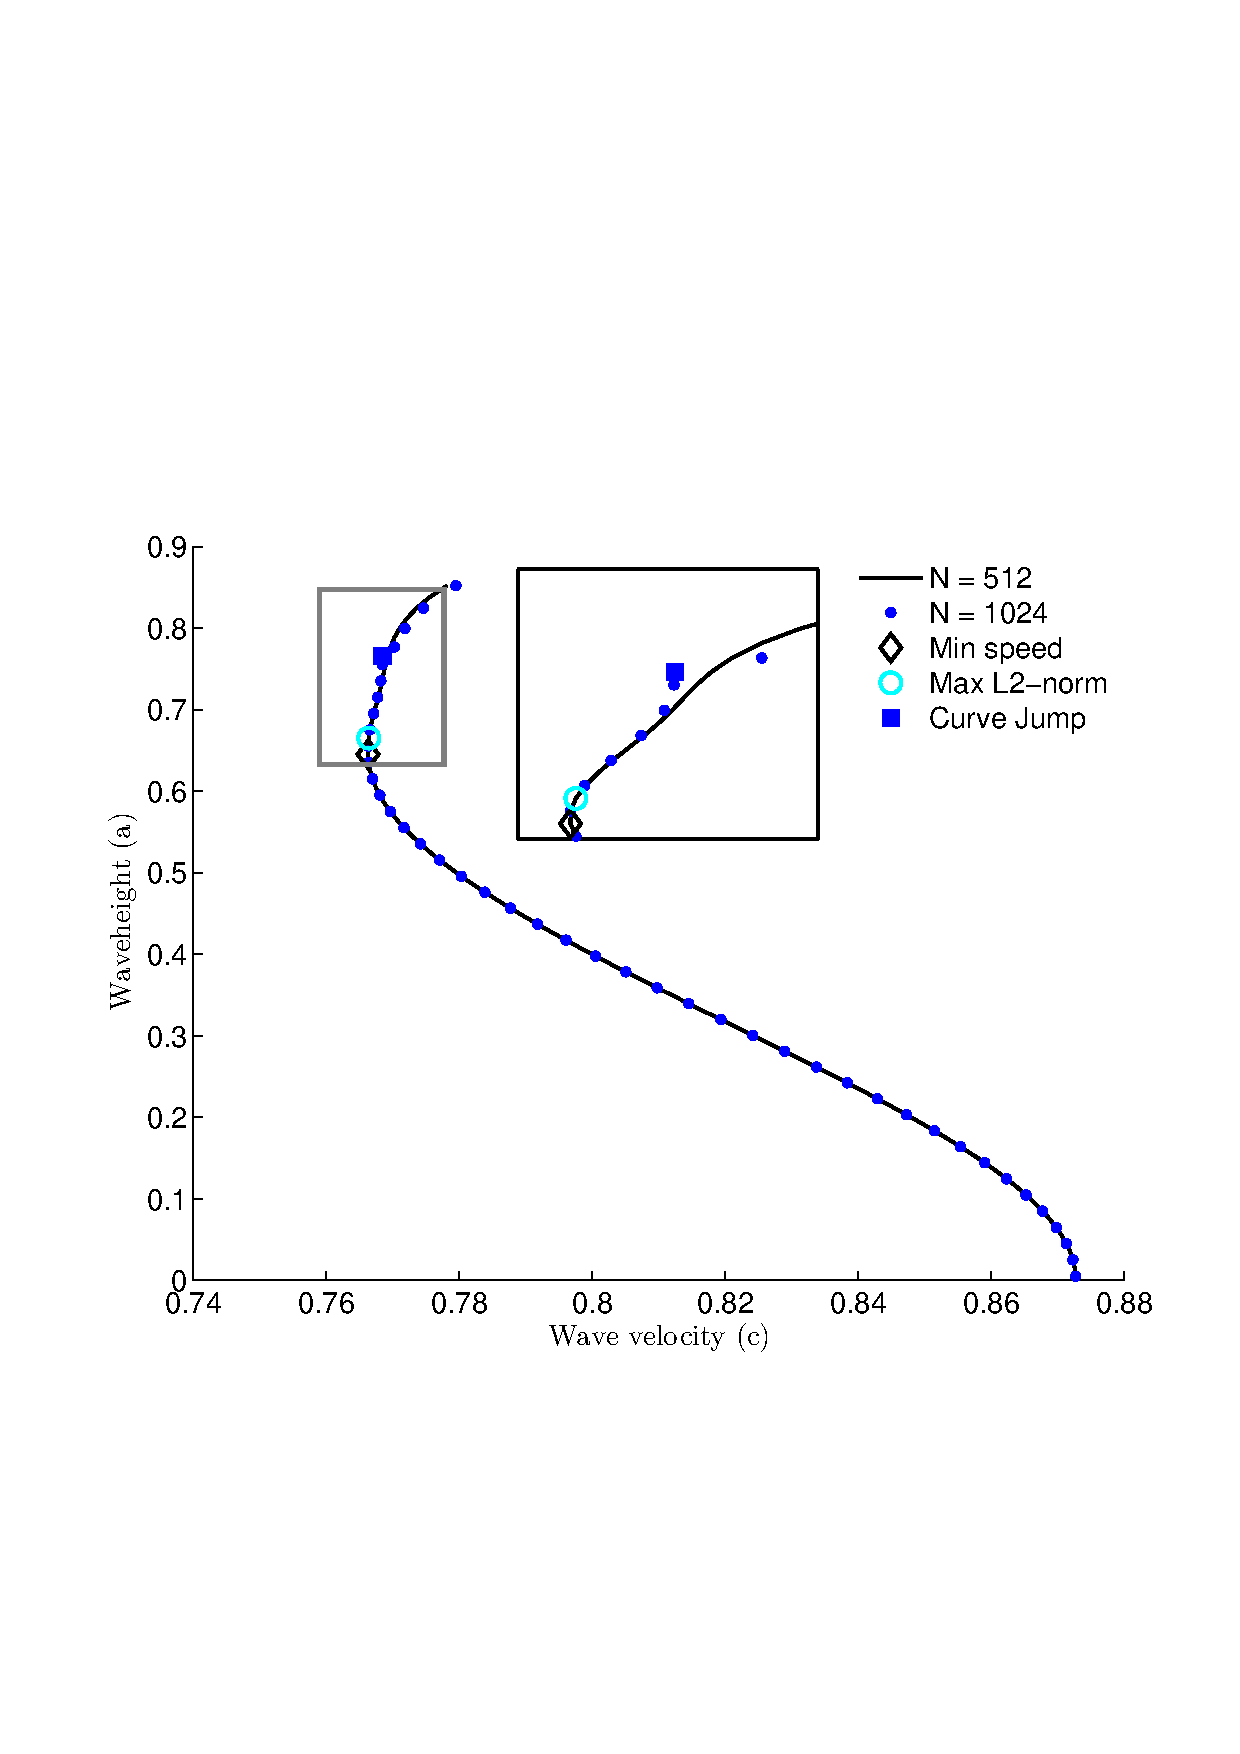
\includegraphics[scale=0.25, trim = 1.2cm 6.5cm 0.6cm 8cm, clip]{512_1024.pdf}
%		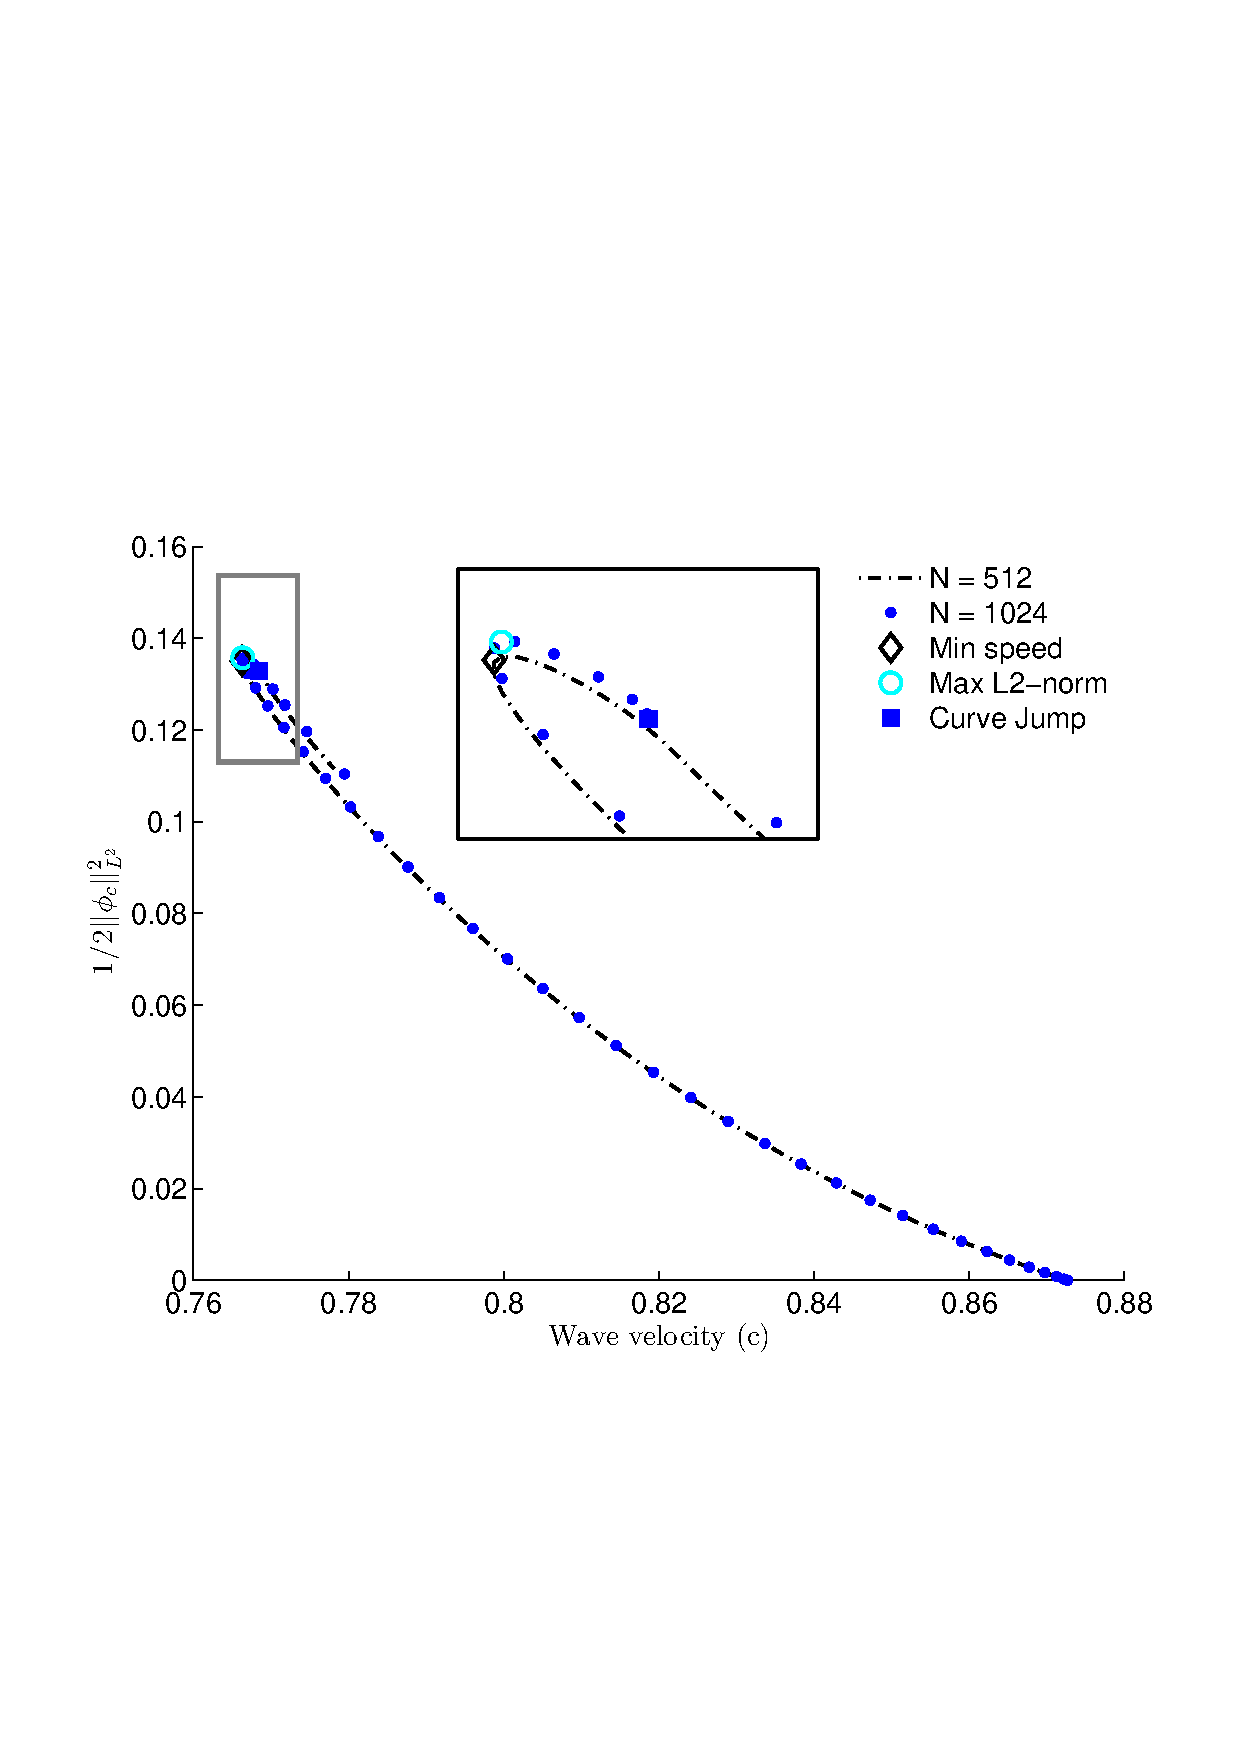
\includegraphics[scale=0.25, trim = 1.2cm 6.5cm 0.6cm 8cm, clip]{L2_512_1024.pdf}\\
%		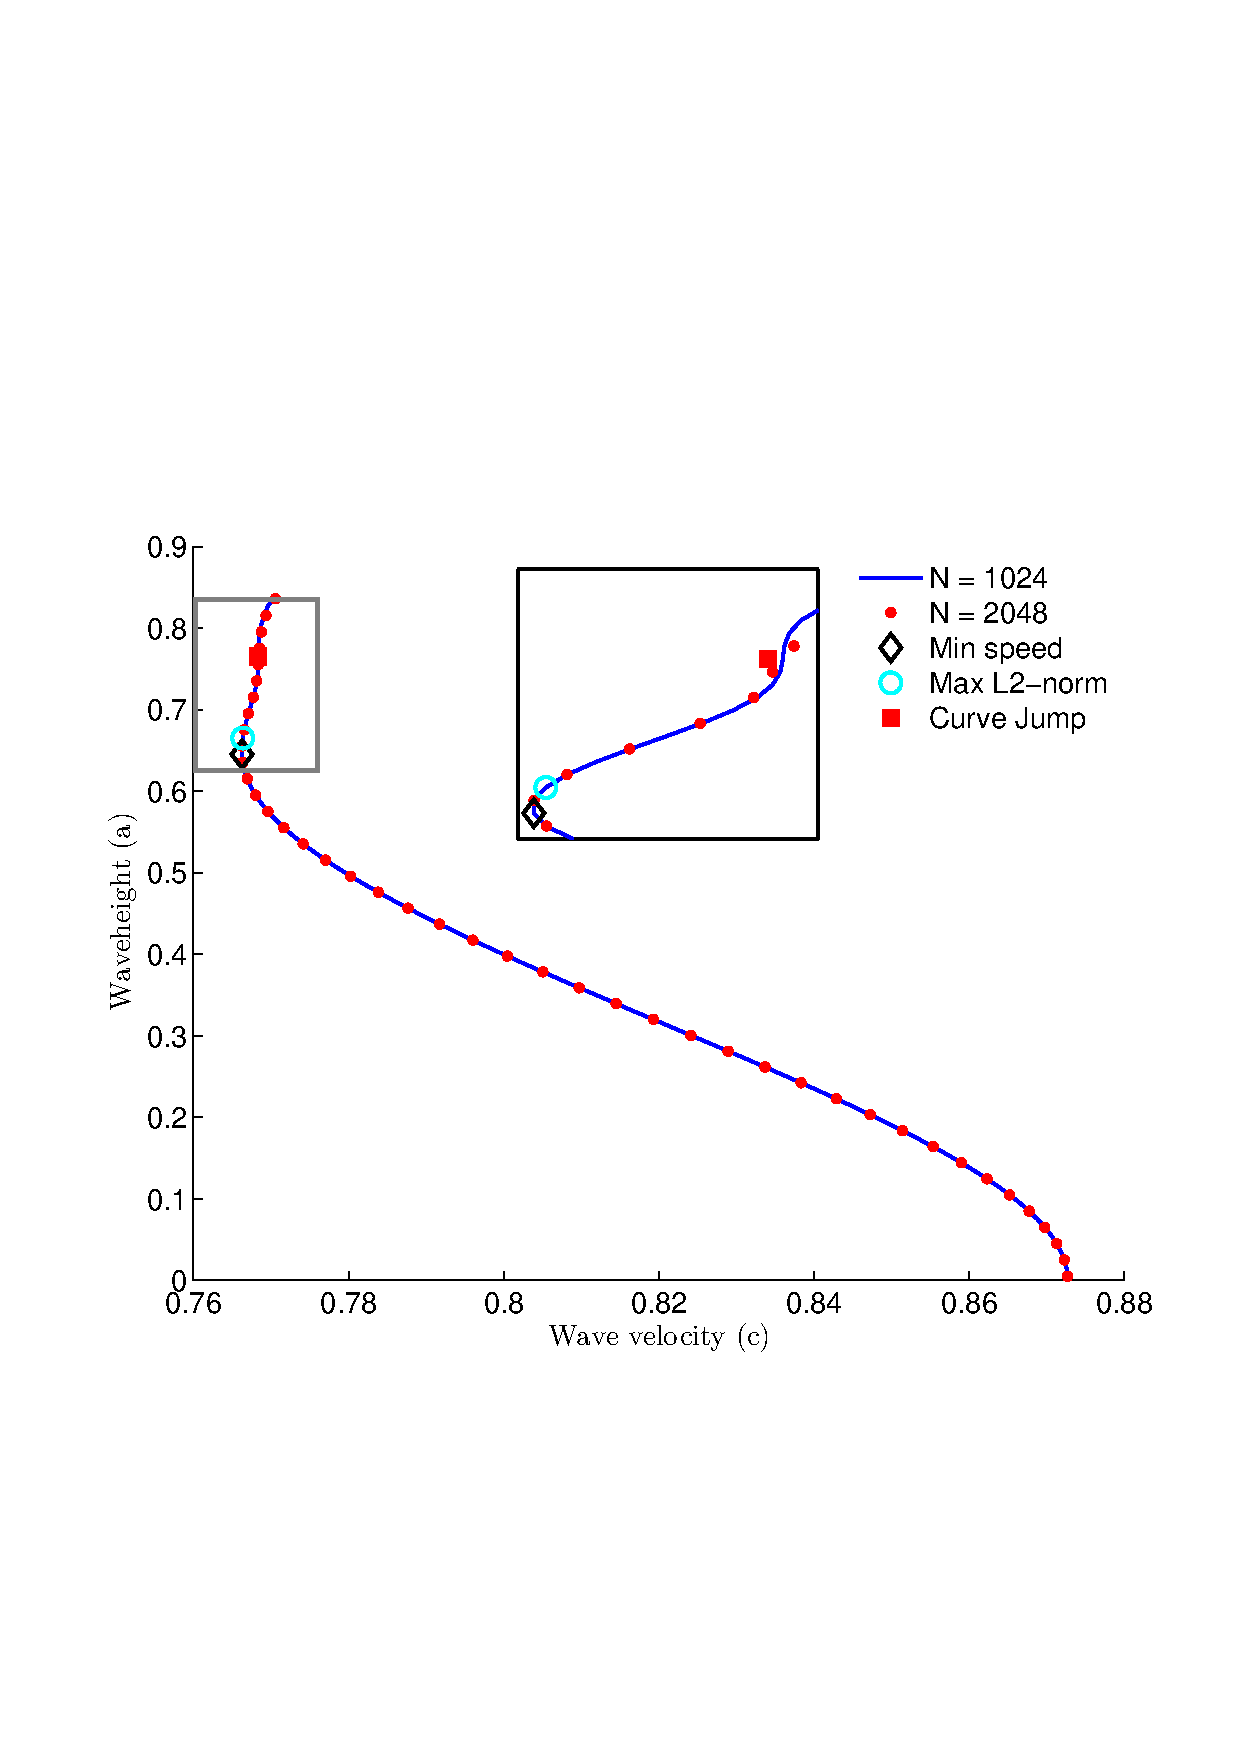
\includegraphics[scale=0.25, trim = 1.2cm 6.5cm 0.6cm 8cm, clip]{1024_2048.pdf}
%		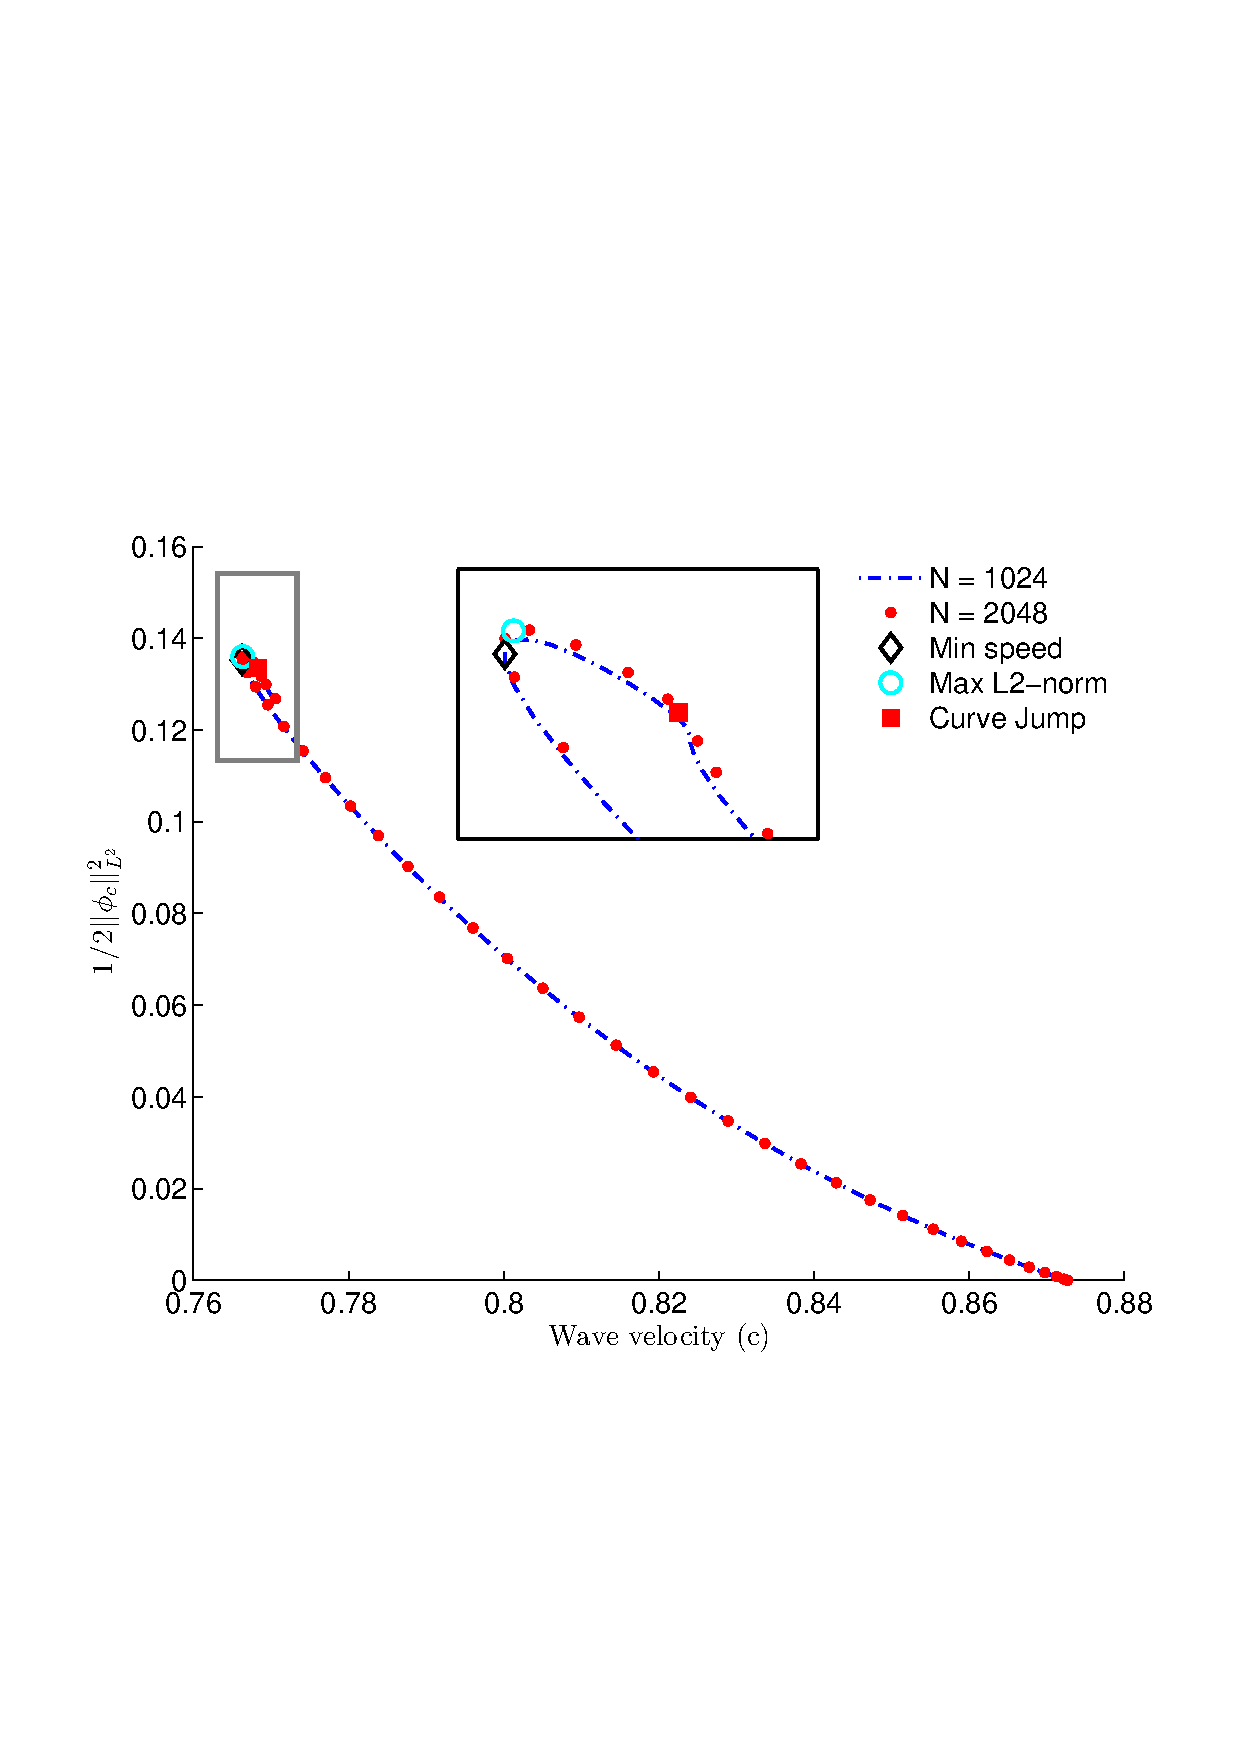
\includegraphics[scale=0.25, trim = 1.2cm 6.5cm 0.6cm 8cm, clip]{L2_1024_2048.pdf}
%	\end{figure}
\end{frame}
%%%%%%%%%%%%%%%%%%%%%%%%%%%%%%%%%%%%%%%%%%%%%%%%%%%%%%%%%%%%%%%%%%%%%%%%%%%%%
%%%%---------------------------------------------------------------------%%%%
%%%%%%%%%%%%%%%%%%%%%%%%%%%%%%%%%%%%%%%%%%%%%%%%%%%%%%%%%%%%%%%%%%%%%%%%%%%%%
\begin{frame}[t]{Stability of solutions: Whitham equation}
Travelling wave solutions to the Whitham equation ($\mbox{wavelength} = 2 \pi$). 

%	\begin{figure}[htbp]    
%		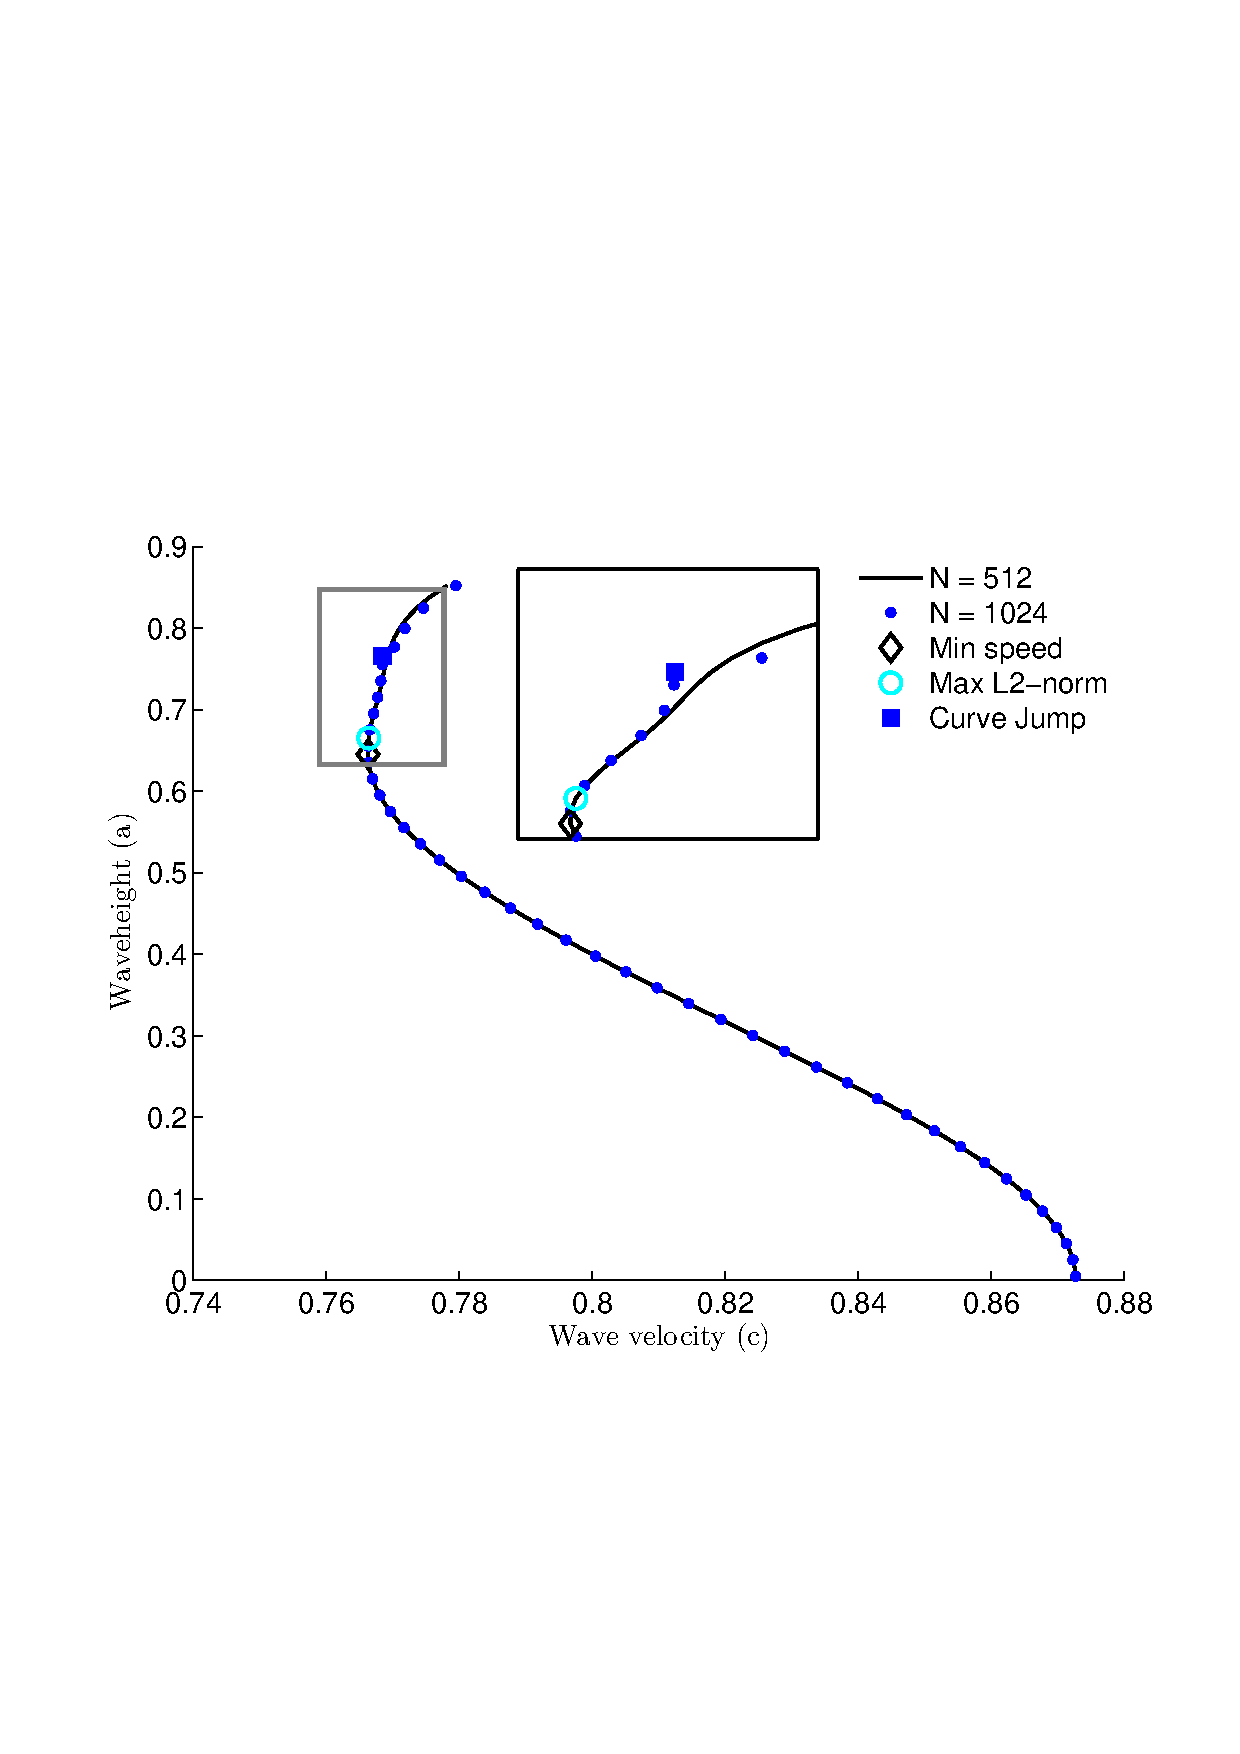
\includegraphics[scale=0.25, trim = 1.2cm 6.5cm 0.6cm 8cm, clip]{512_1024.pdf}
%		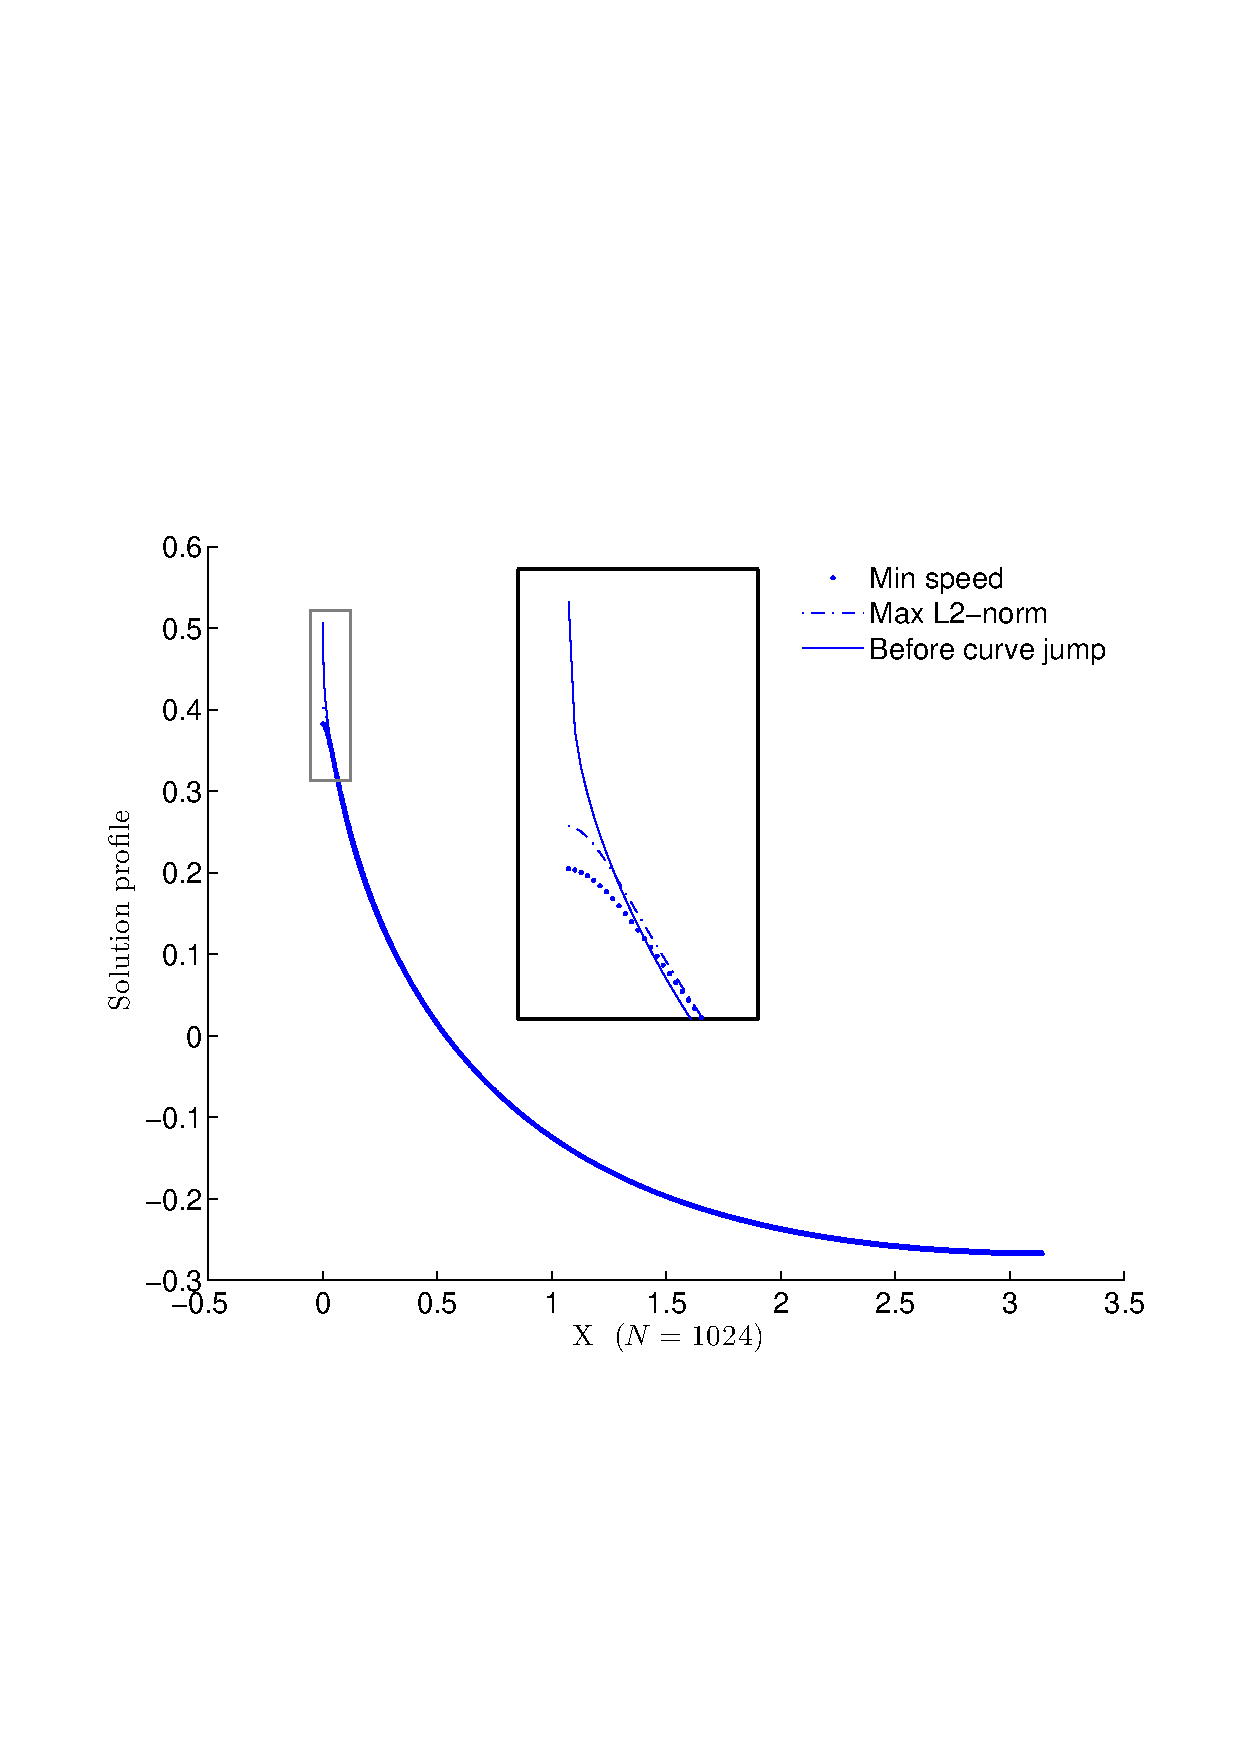
\includegraphics[scale=0.35, trim = 1.2cm 6.5cm 0.6cm 8cm, clip]{1024_waves_1.pdf}
%	\end{figure}
\end{frame}
%%%%%%%%%%%%%%%%%%%%%%%%%%%%%%%%%%%%%%%%%%%%%%%%%%%%%%%%%%%%%%%%%%%%%%%%%%%%%
%%%%---------------------------------------------------------------------%%%%
%%%%%%%%%%%%%%%%%%%%%%%%%%%%%%%%%%%%%%%%%%%%%%%%%%%%%%%%%%%%%%%%%%%%%%%%%%%%%
\begin{frame}[t]{Stability of solutions: Whitham equation}
Travelling wave solutions to the Whitham equation ($\mbox{wavelength} = 2 \pi$). 

%	\begin{figure}[htbp]    
%		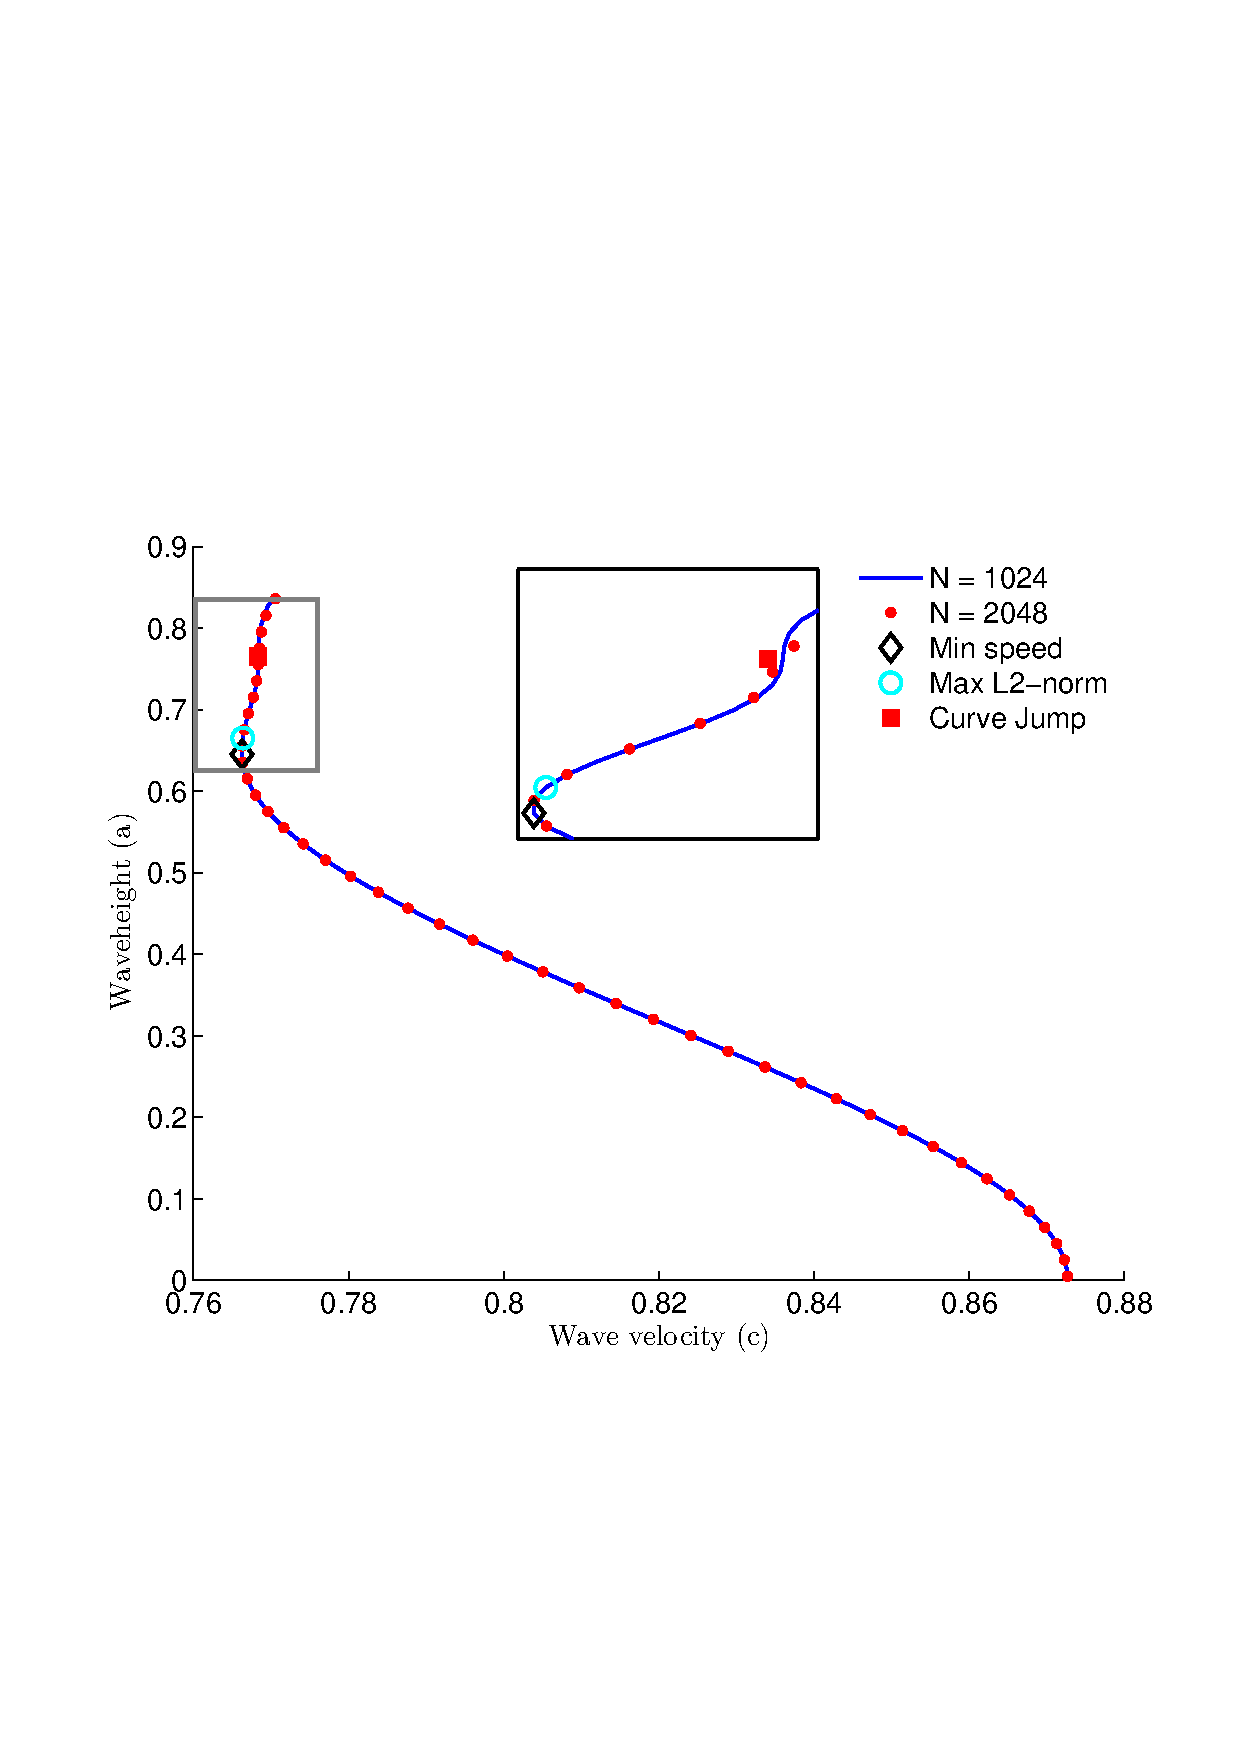
\includegraphics[scale=0.25, trim = 1.2cm 6.5cm 0.6cm 8cm, clip]{1024_2048.pdf}
%		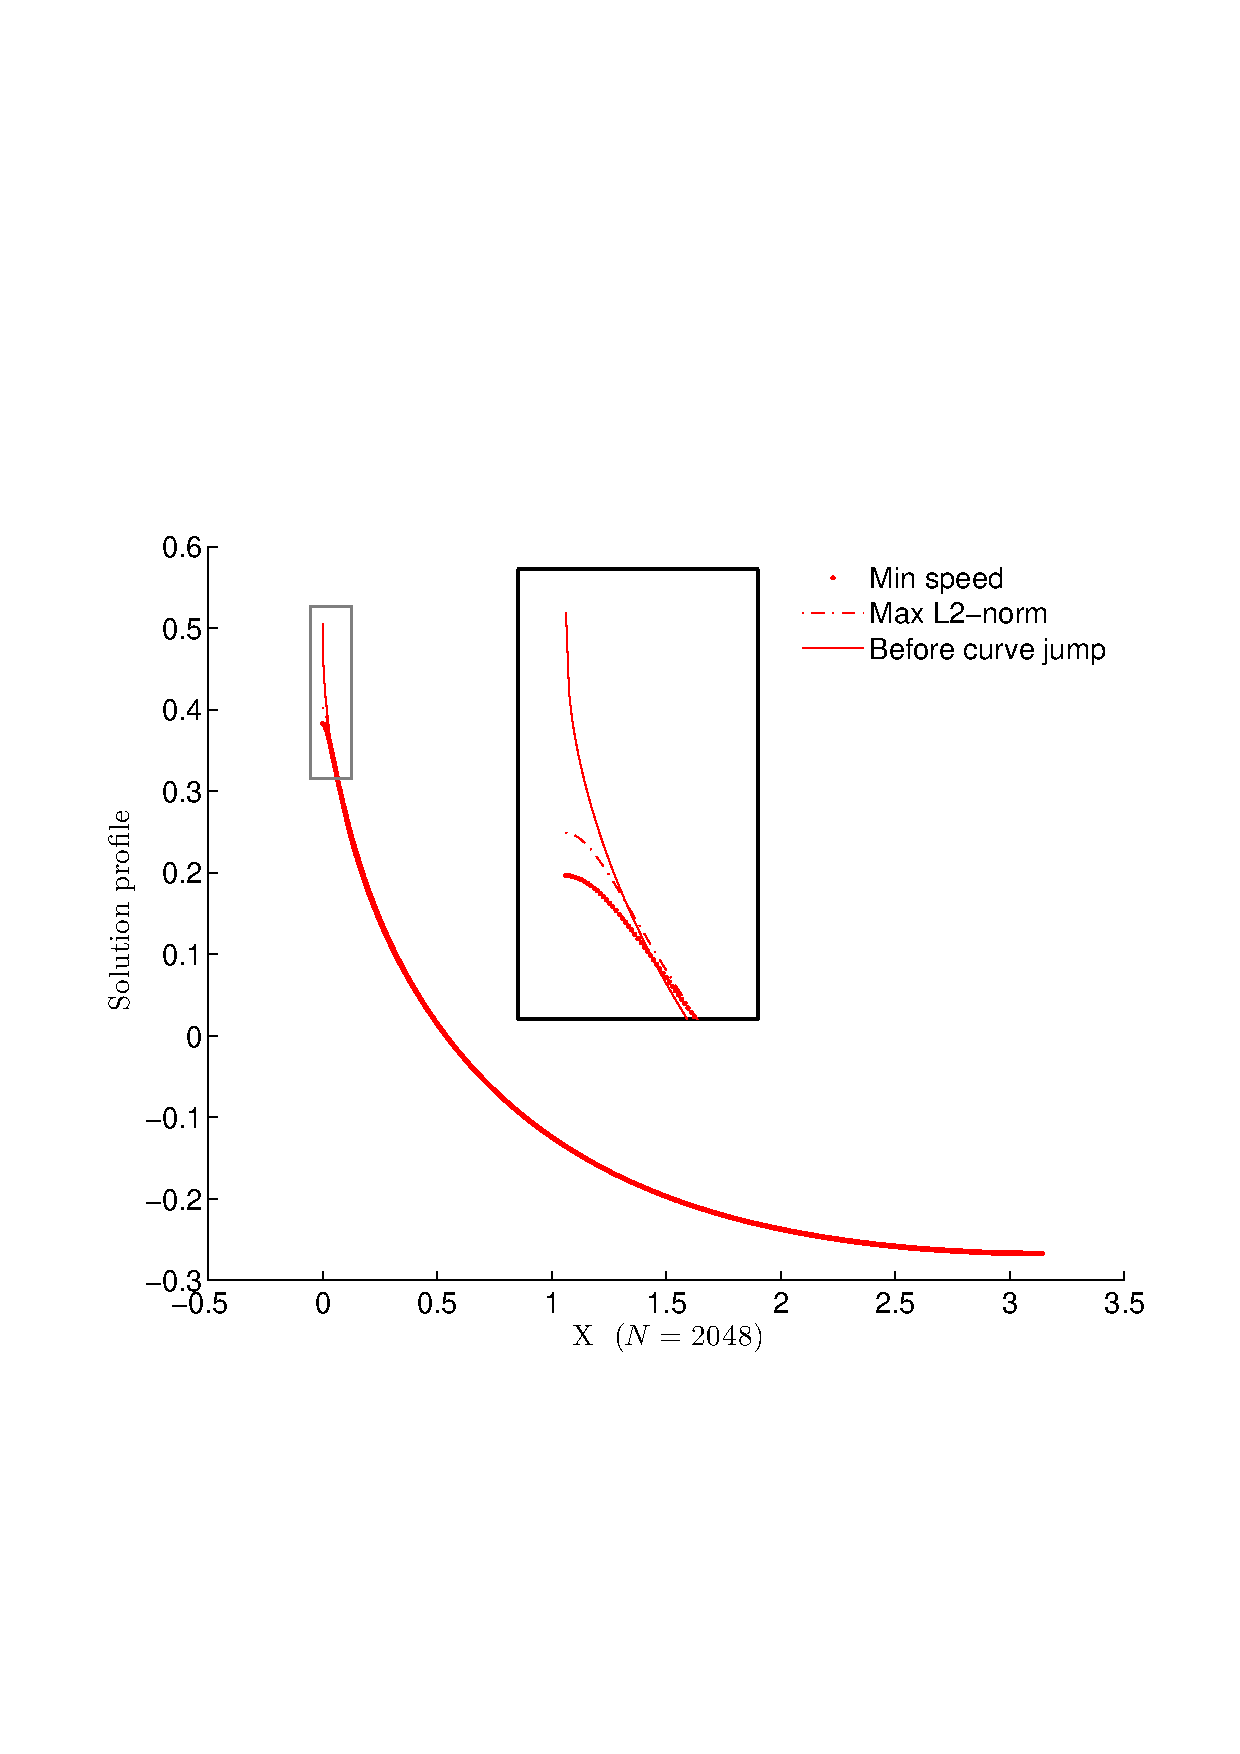
\includegraphics[scale=0.35, trim = 1.2cm 6.5cm 0.6cm 8cm, clip]{2048_waves_1.pdf}
%	\end{figure}
\end{frame}
%%%%%%%%%%%%%%%%%%%%%%%%%%%%%%%%%%%%%%%%%%%%%%%%%%%%%%%%%%%%%%%%%%%%%%%%%%%%%
%%%%---------------------------------------------------------------------%%%%
%%%%%%%%%%%%%%%%%%%%%%%%%%%%%%%%%%%%%%%%%%%%%%%%%%%%%%%%%%%%%%%%%%%%%%%%%%%%%
\begin{frame}[t]{Stability of solutions: Whitham equation}
What happens after the bifurcation curve "jump"?

%	\begin{figure}[htbp]    
%		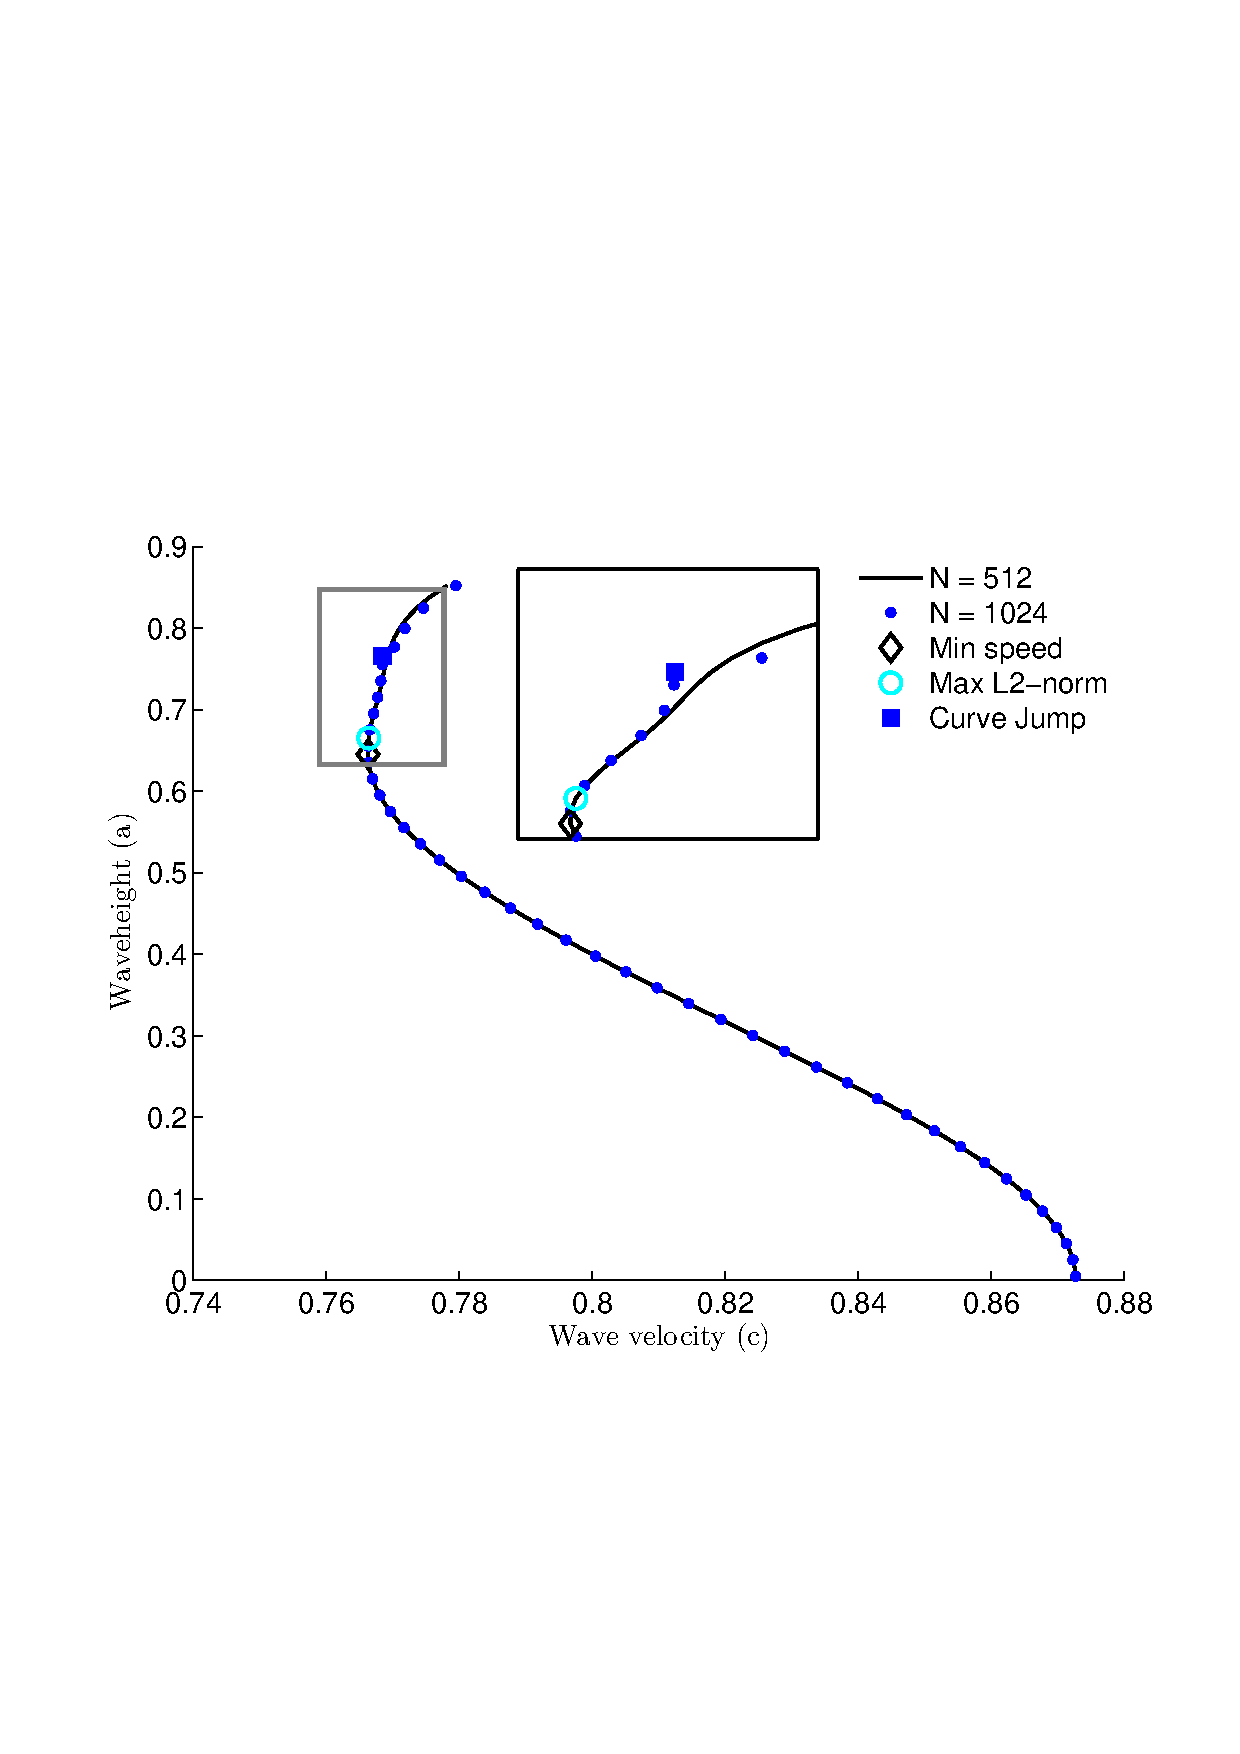
\includegraphics[scale=0.2, trim = 1.2cm 6.5cm 0.6cm 8cm, clip]{512_1024.pdf}
%		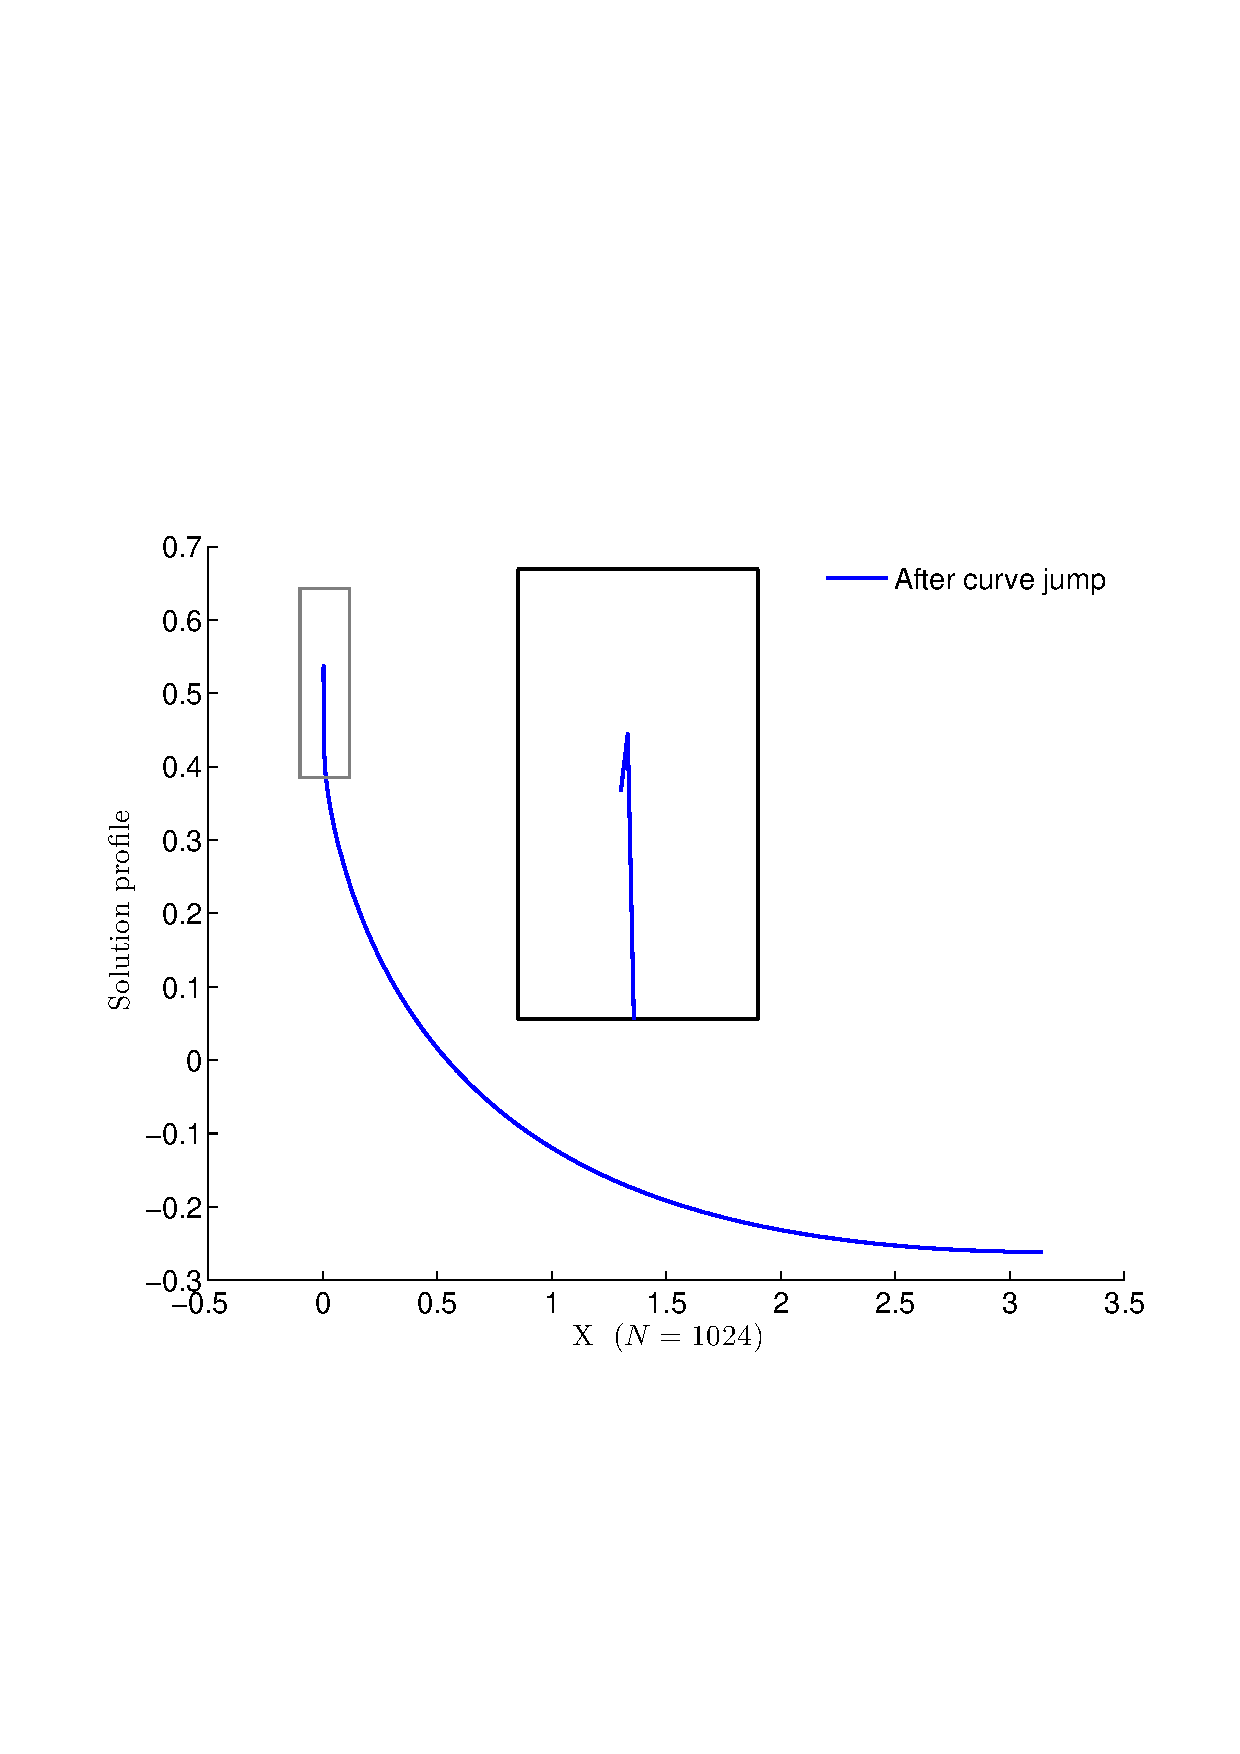
\includegraphics[scale=0.35, trim = 1.2cm 6.5cm 0.6cm 8cm, clip]{1024_waves_2.pdf}
%	\end{figure}
\end{frame}
%%%%%%%%%%%%%%%%%%%%%%%%%%%%%%%%%%%%%%%%%%%%%%%%%%%%%%%%%%%%%%%%%%%%%%%%%%%%%
%%%%---------------------------------------------------------------------%%%%
%%%%%%%%%%%%%%%%%%%%%%%%%%%%%%%%%%%%%%%%%%%%%%%%%%%%%%%%%%%%%%%%%%%%%%%%%%%%%
\begin{frame}[t]{Stability of solutions: Whitham equation}
%	\begin{figure}[htbp]    
%		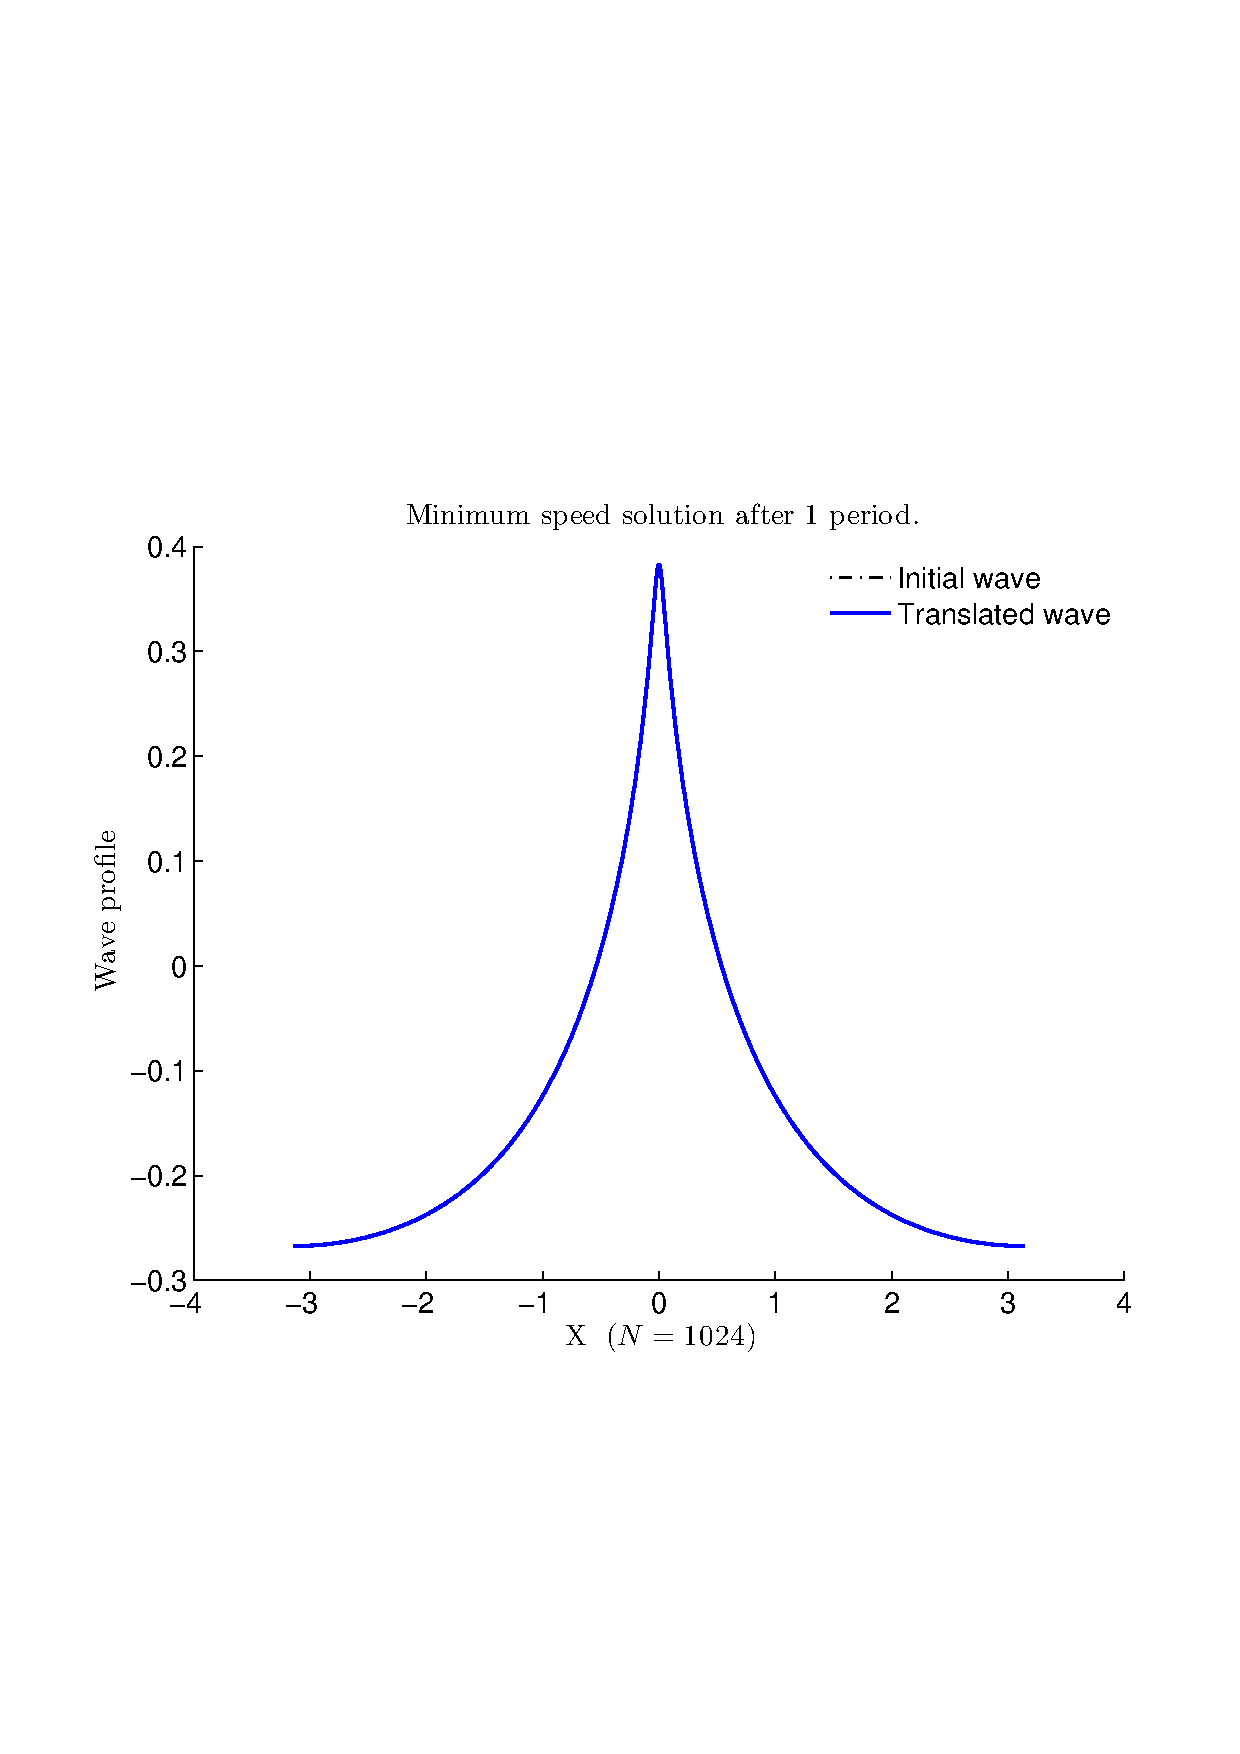
\includegraphics[scale=0.2, trim = 1.2cm 6.5cm 0.6cm 8cm, clip]{1024_full_1p_1.pdf}
%		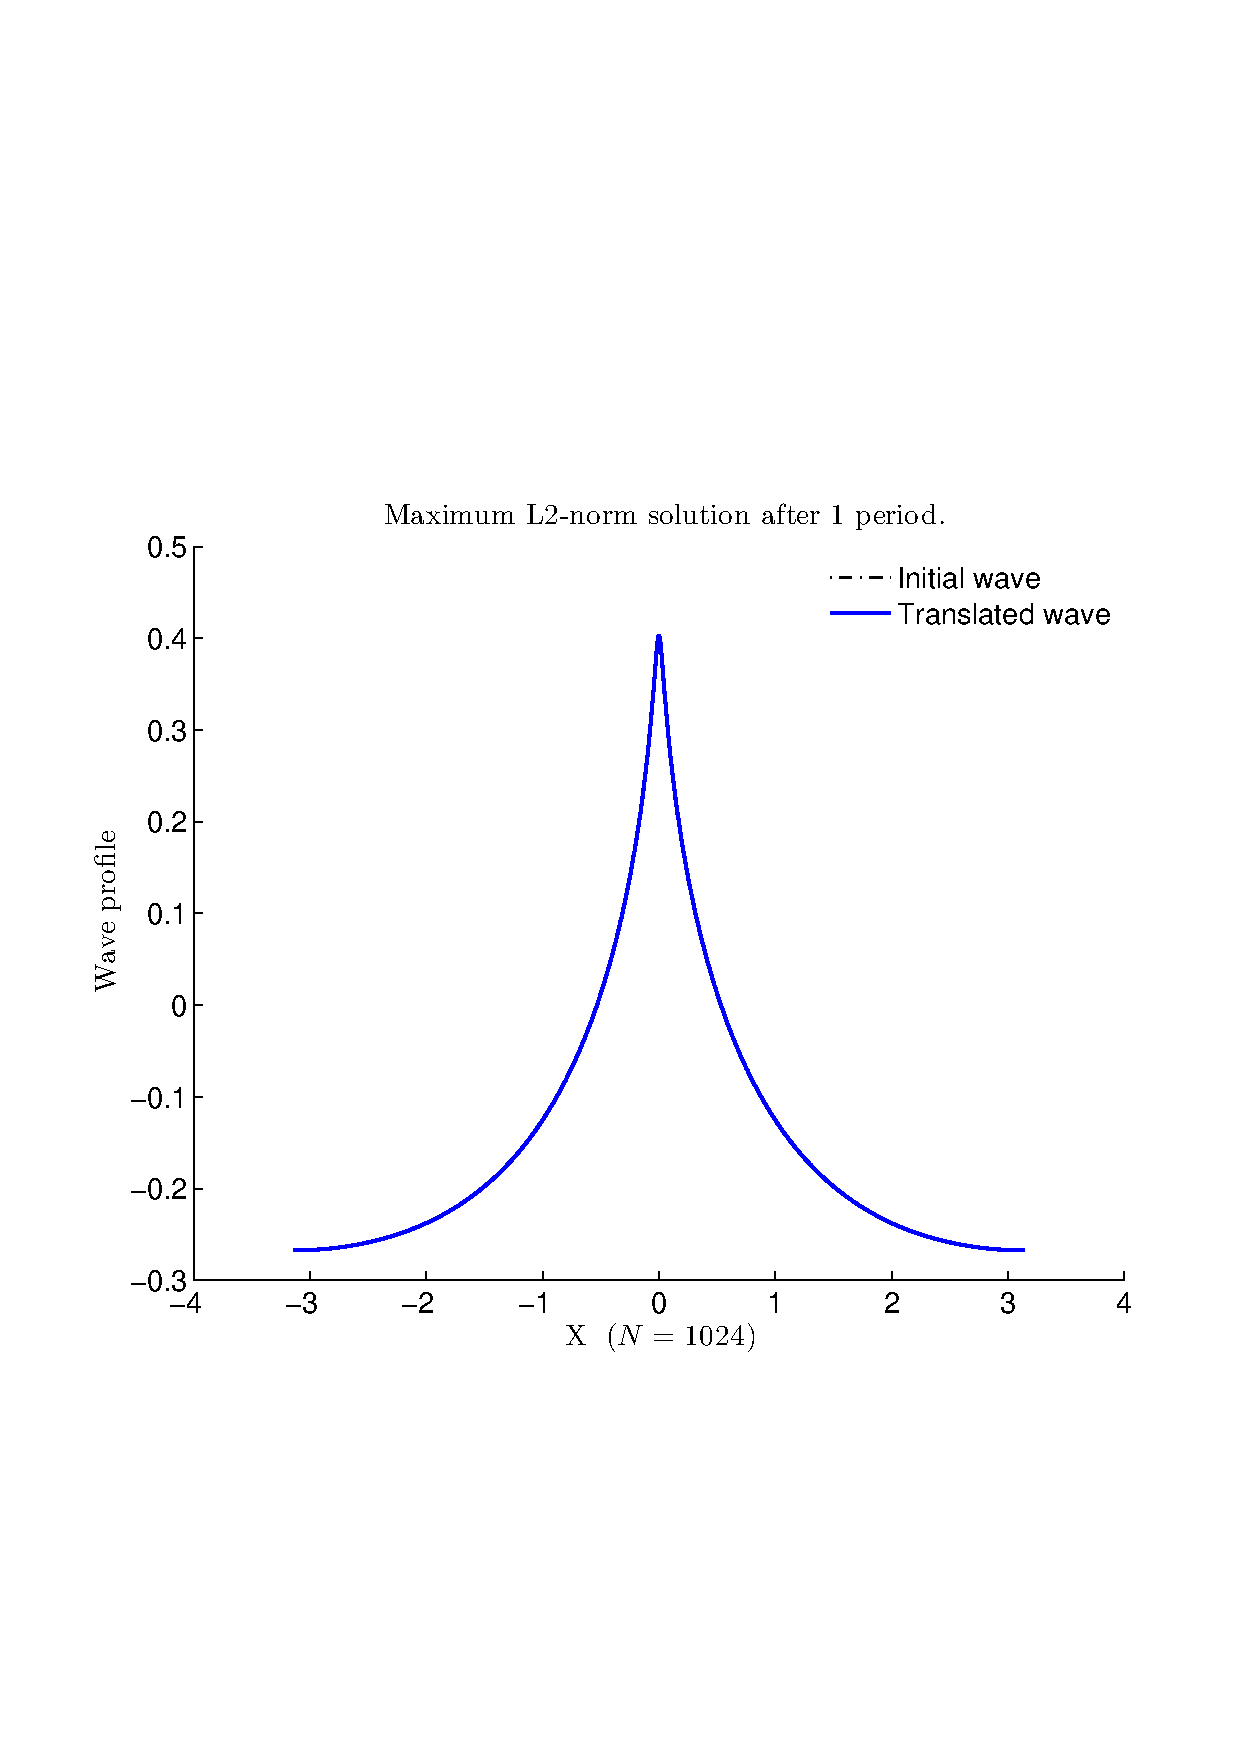
\includegraphics[scale=0.2, trim = 1.2cm 6.5cm 0.6cm 8cm, clip]{1024_full_1p_2.pdf}
%		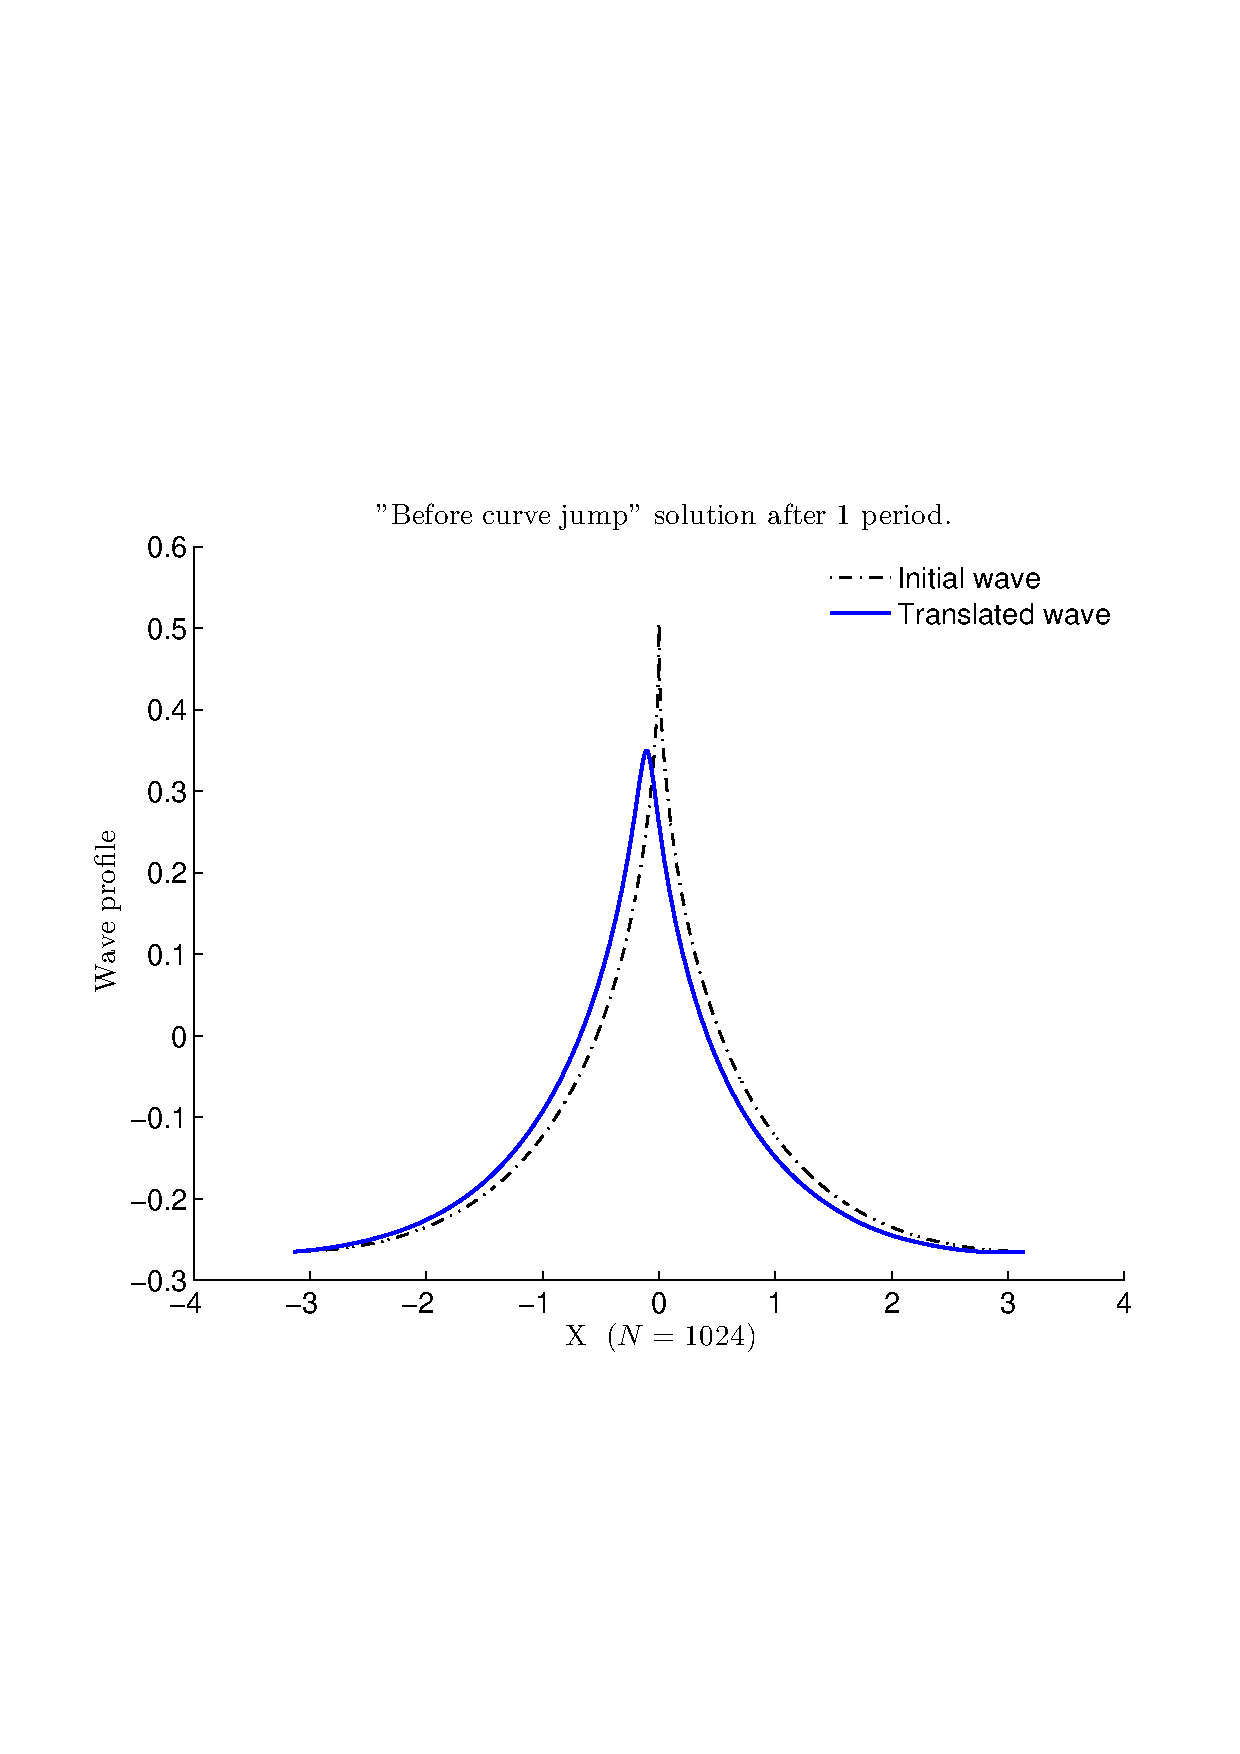
\includegraphics[scale=0.2, trim = 1.2cm 6.5cm 0.6cm 8cm, clip]{1024_full_1p_3.pdf}
%	\end{figure}
%\begin{figure}[htbp]    
%		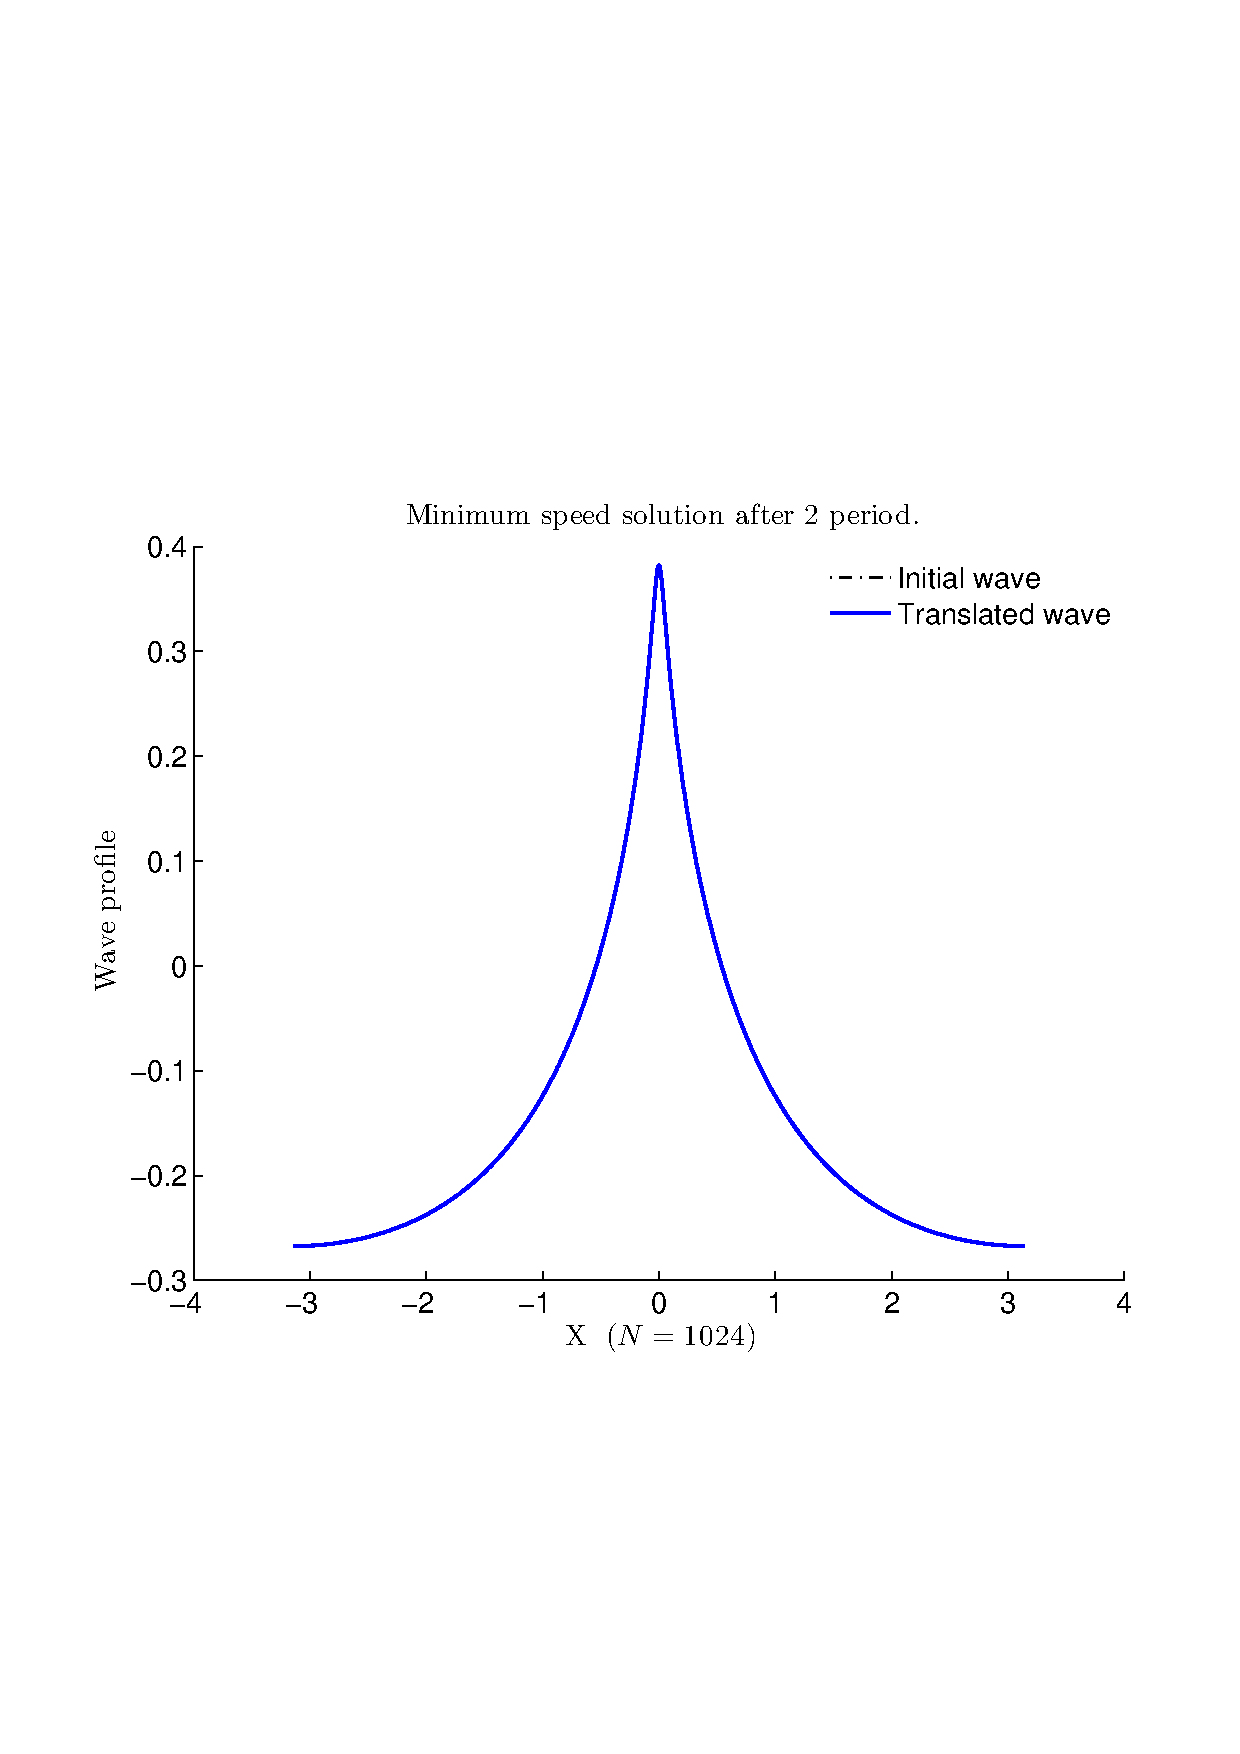
\includegraphics[scale=0.2, trim = 1.2cm 6.5cm 0.6cm 8cm, clip]{1024_full_2p_1.pdf}
%		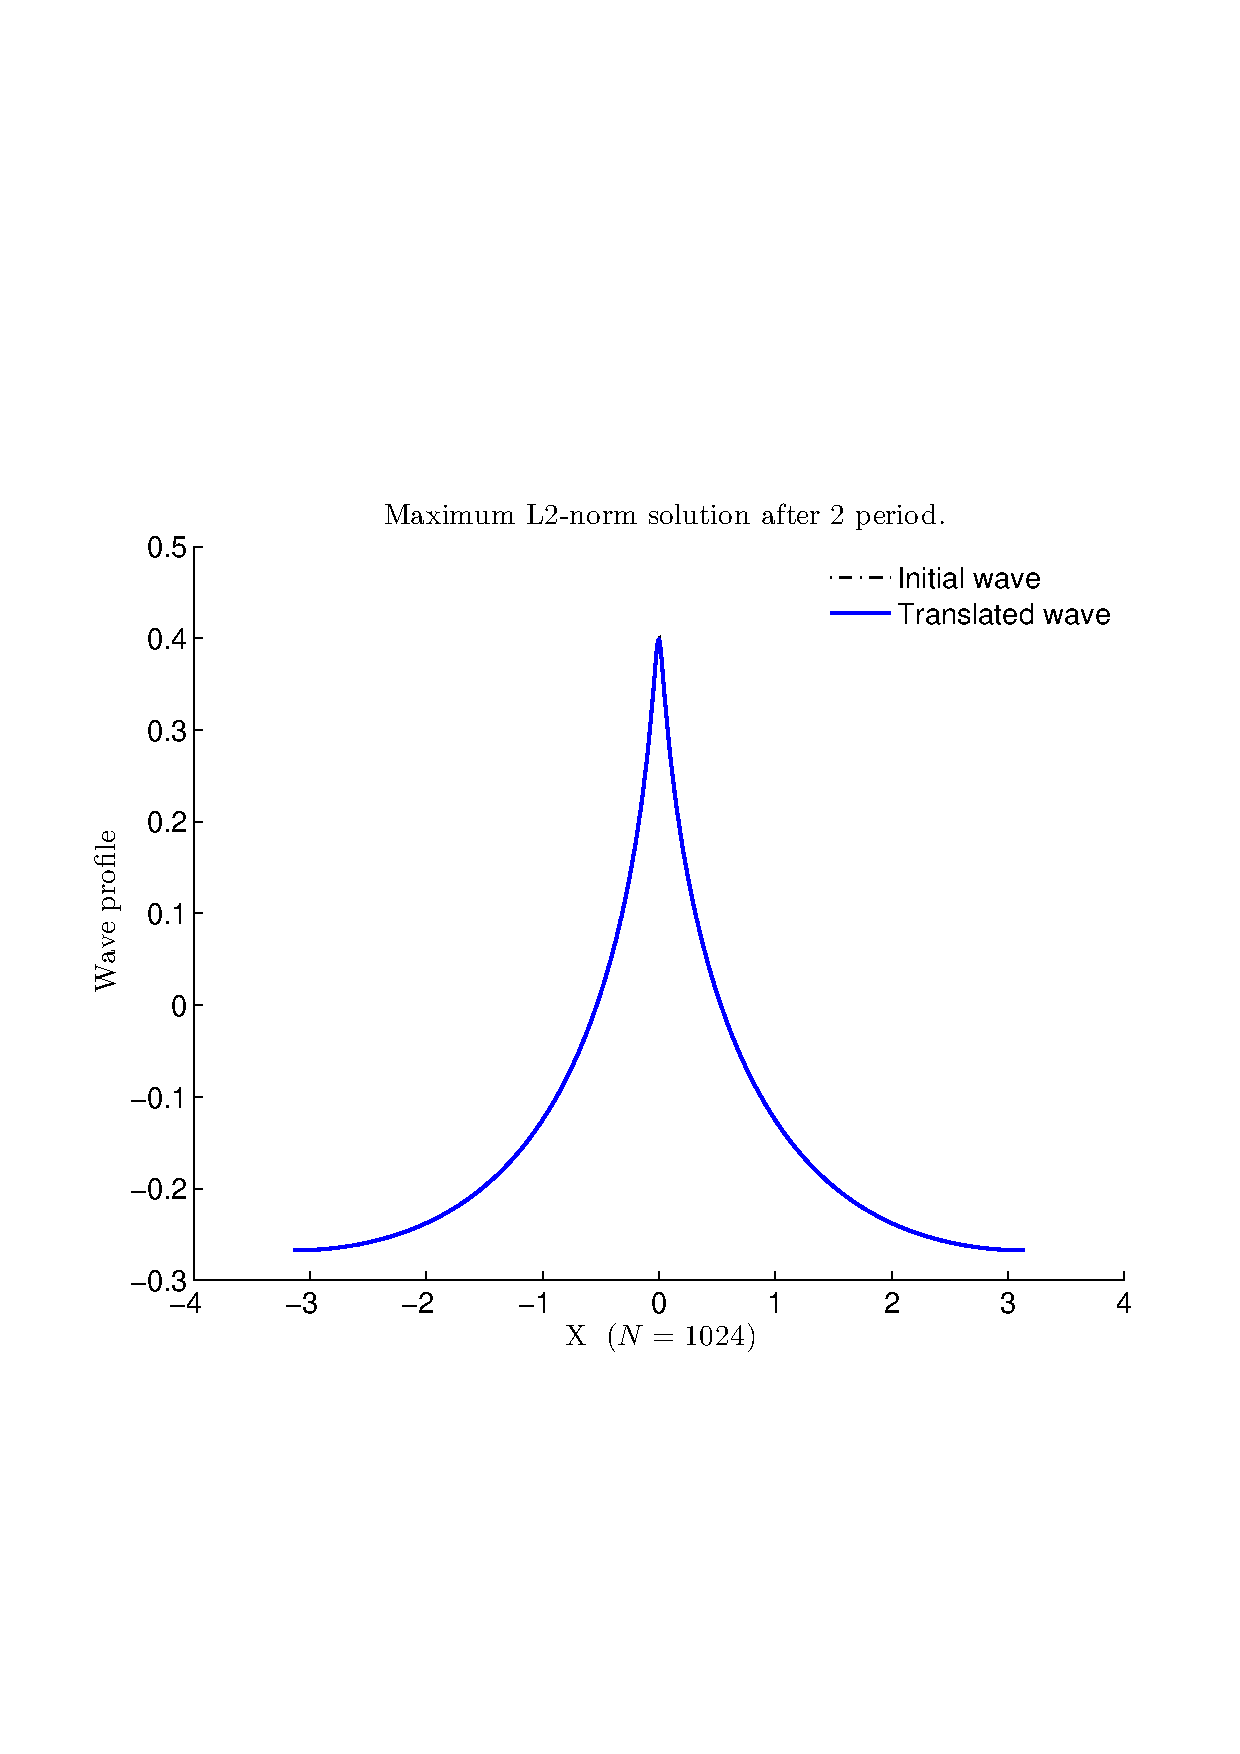
\includegraphics[scale=0.2, trim = 1.2cm 6.5cm 0.6cm 8cm, clip]{1024_full_2p_2.pdf}
%		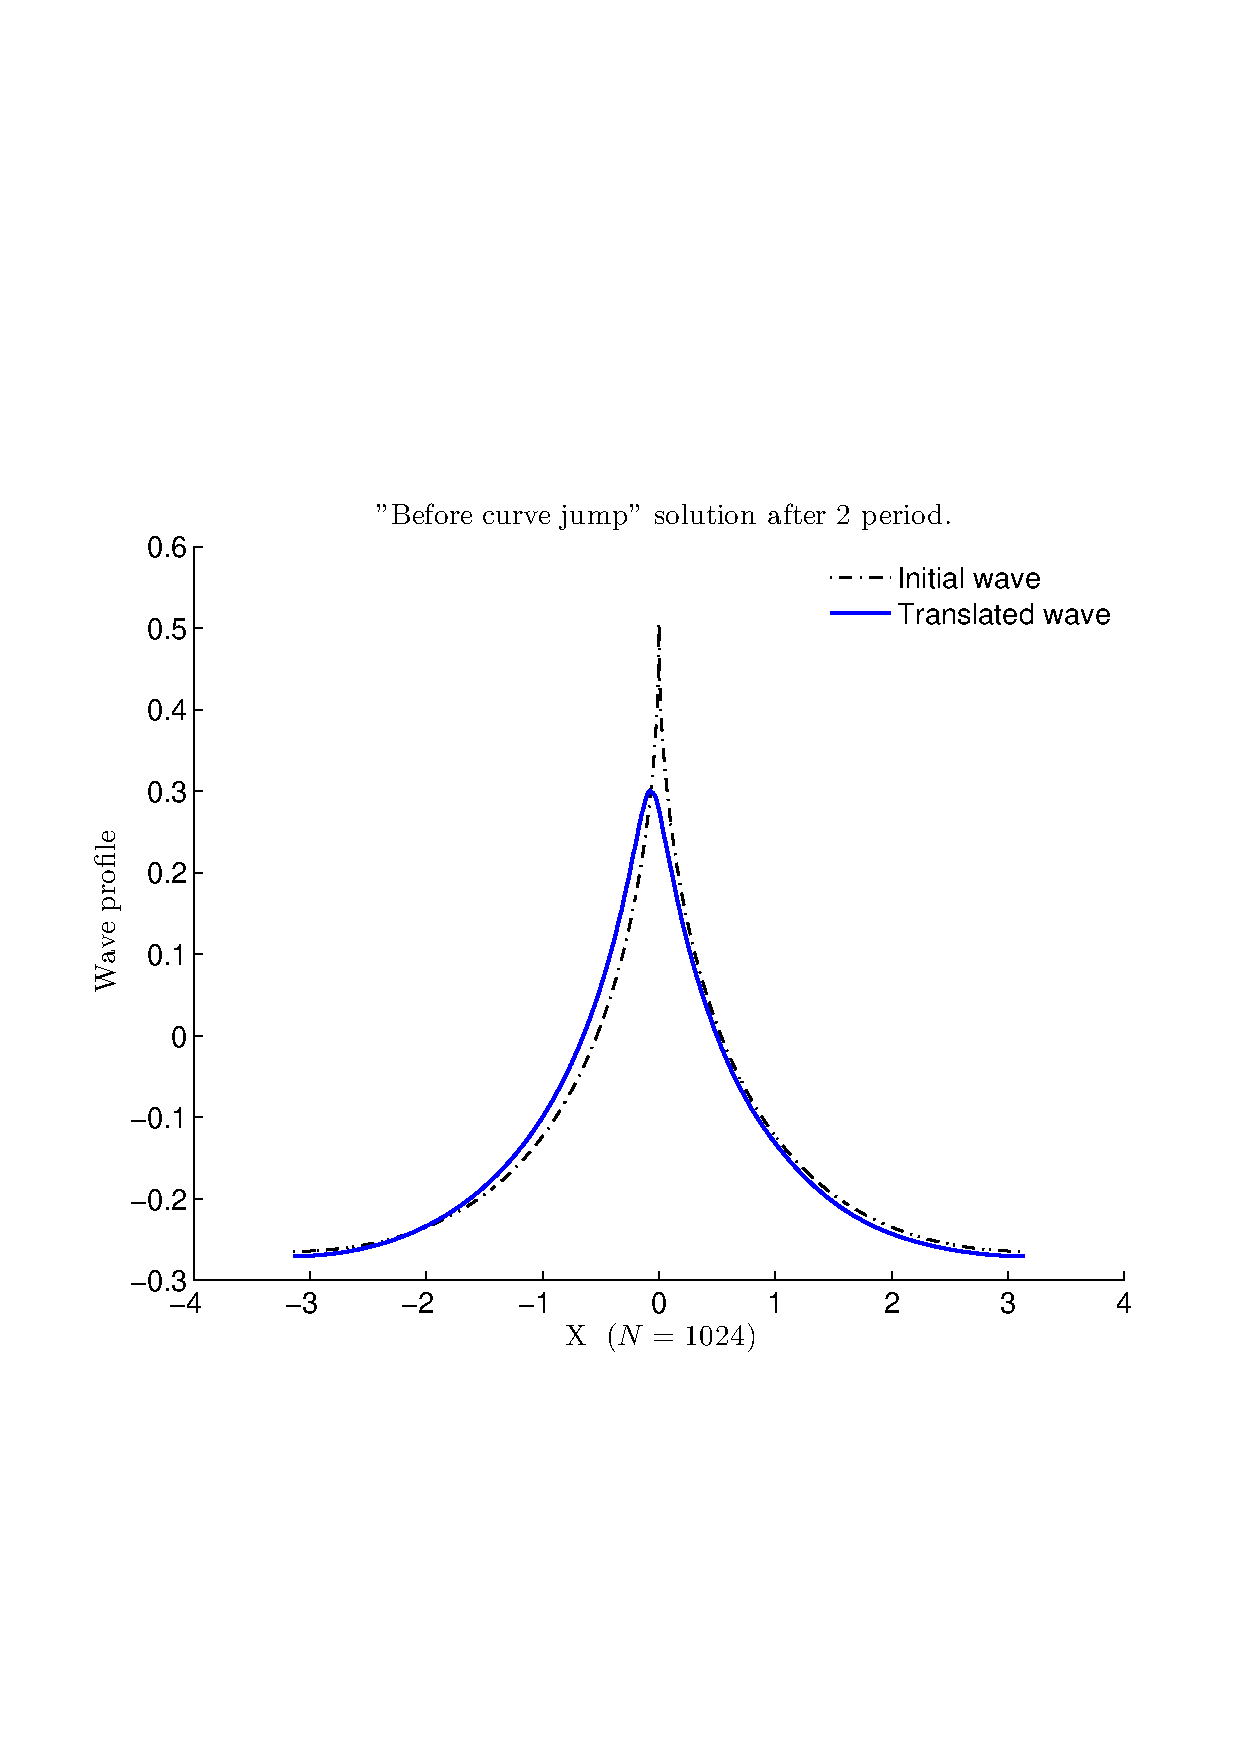
\includegraphics[scale=0.2, trim = 1.2cm 6.5cm 0.6cm 8cm, clip]{1024_full_2p_3.pdf}
%\end{figure}
\end{frame}
%%%%%%%%%%%%%%%%%%%%%%%%%%%%%%%%%%%%%%%%%%%%%%%%%%%%%%%%%%%%%%%%%%%%%%%%%%%%%
%%%%---------------------------------------------------------------------%%%%
%%%%%%%%%%%%%%%%%%%%%%%%%%%%%%%%%%%%%%%%%%%%%%%%%%%%%%%%%%%%%%%%%%%%%%%%%%%%%
\begin{frame}[t]{Stability of solutions: Whitham equation}
%\begin{figure}[htbp]    
%		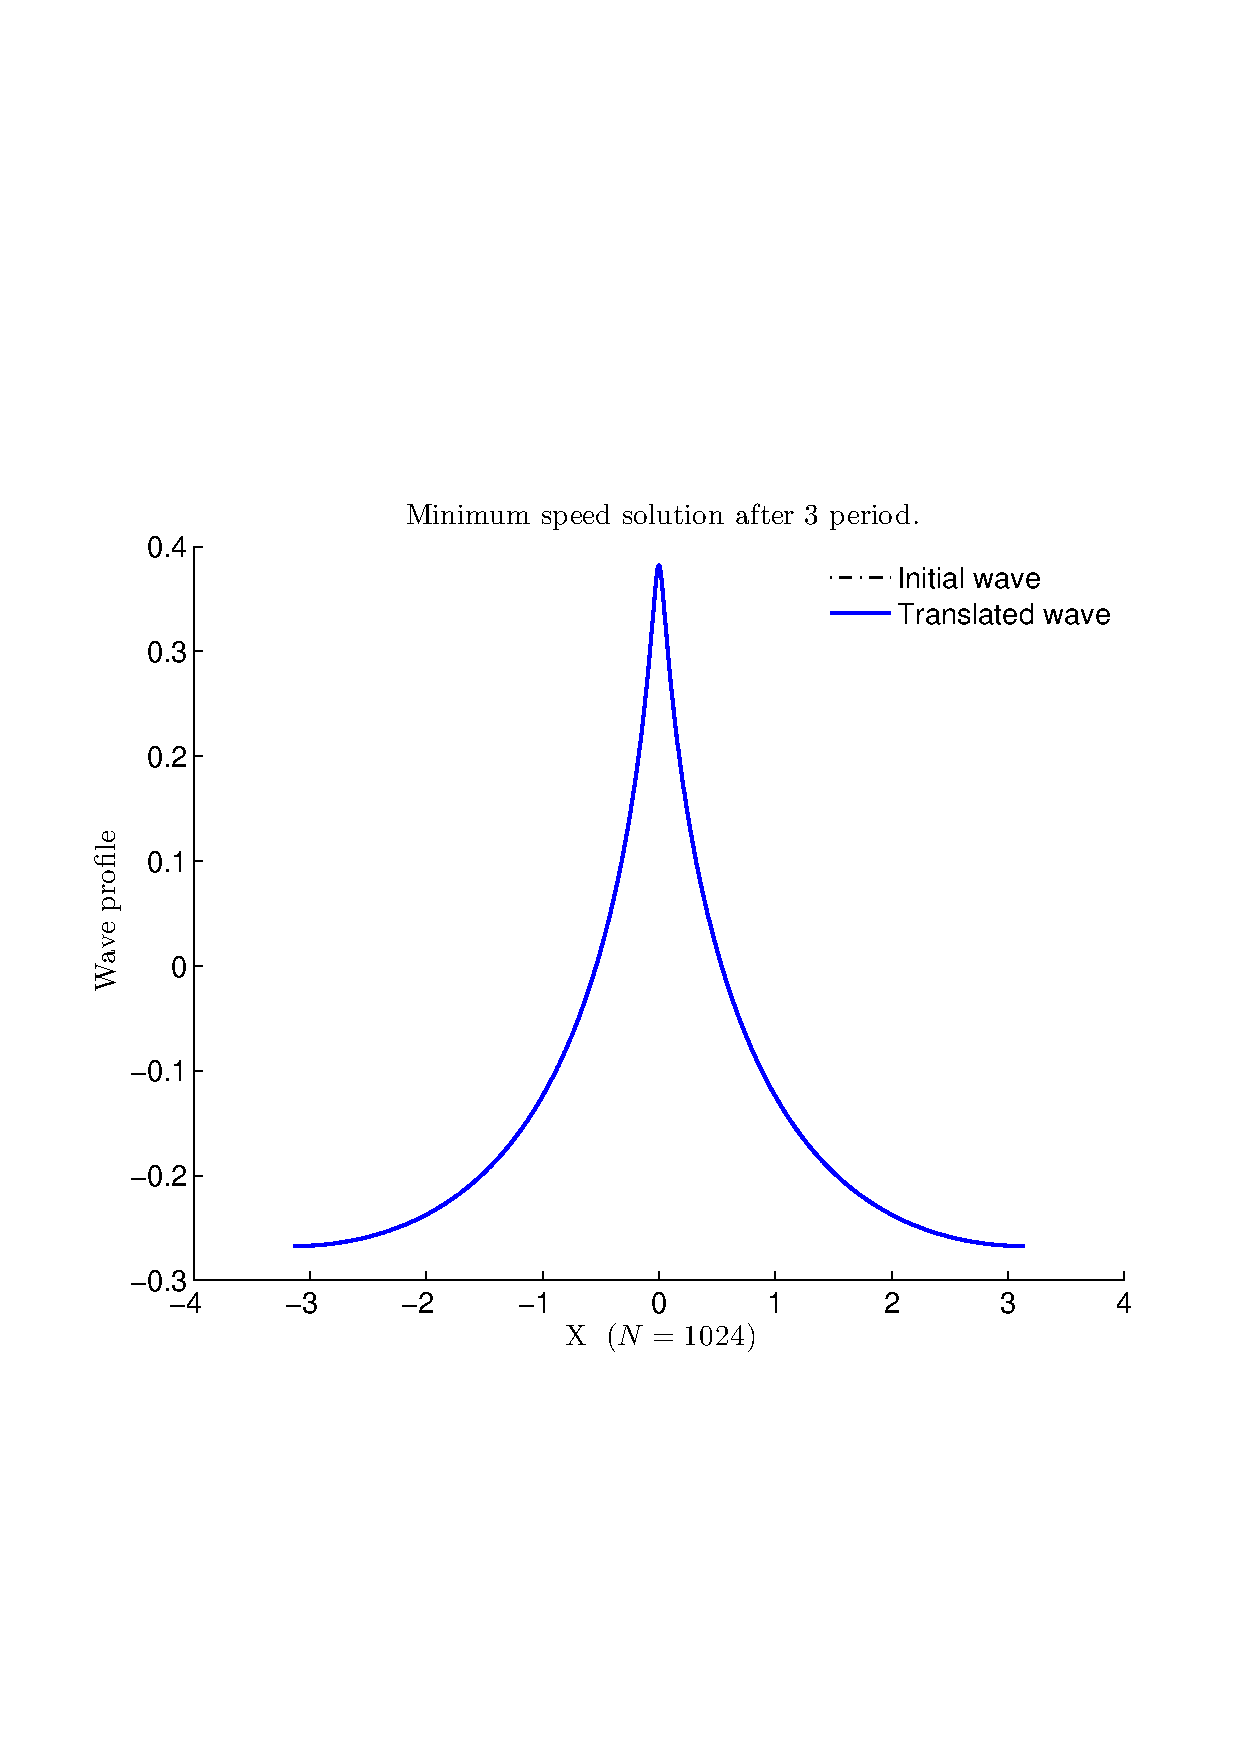
\includegraphics[scale=0.2, trim = 1.2cm 6.5cm 0.6cm 8cm, clip]{1024_full_3p_1.pdf}
%		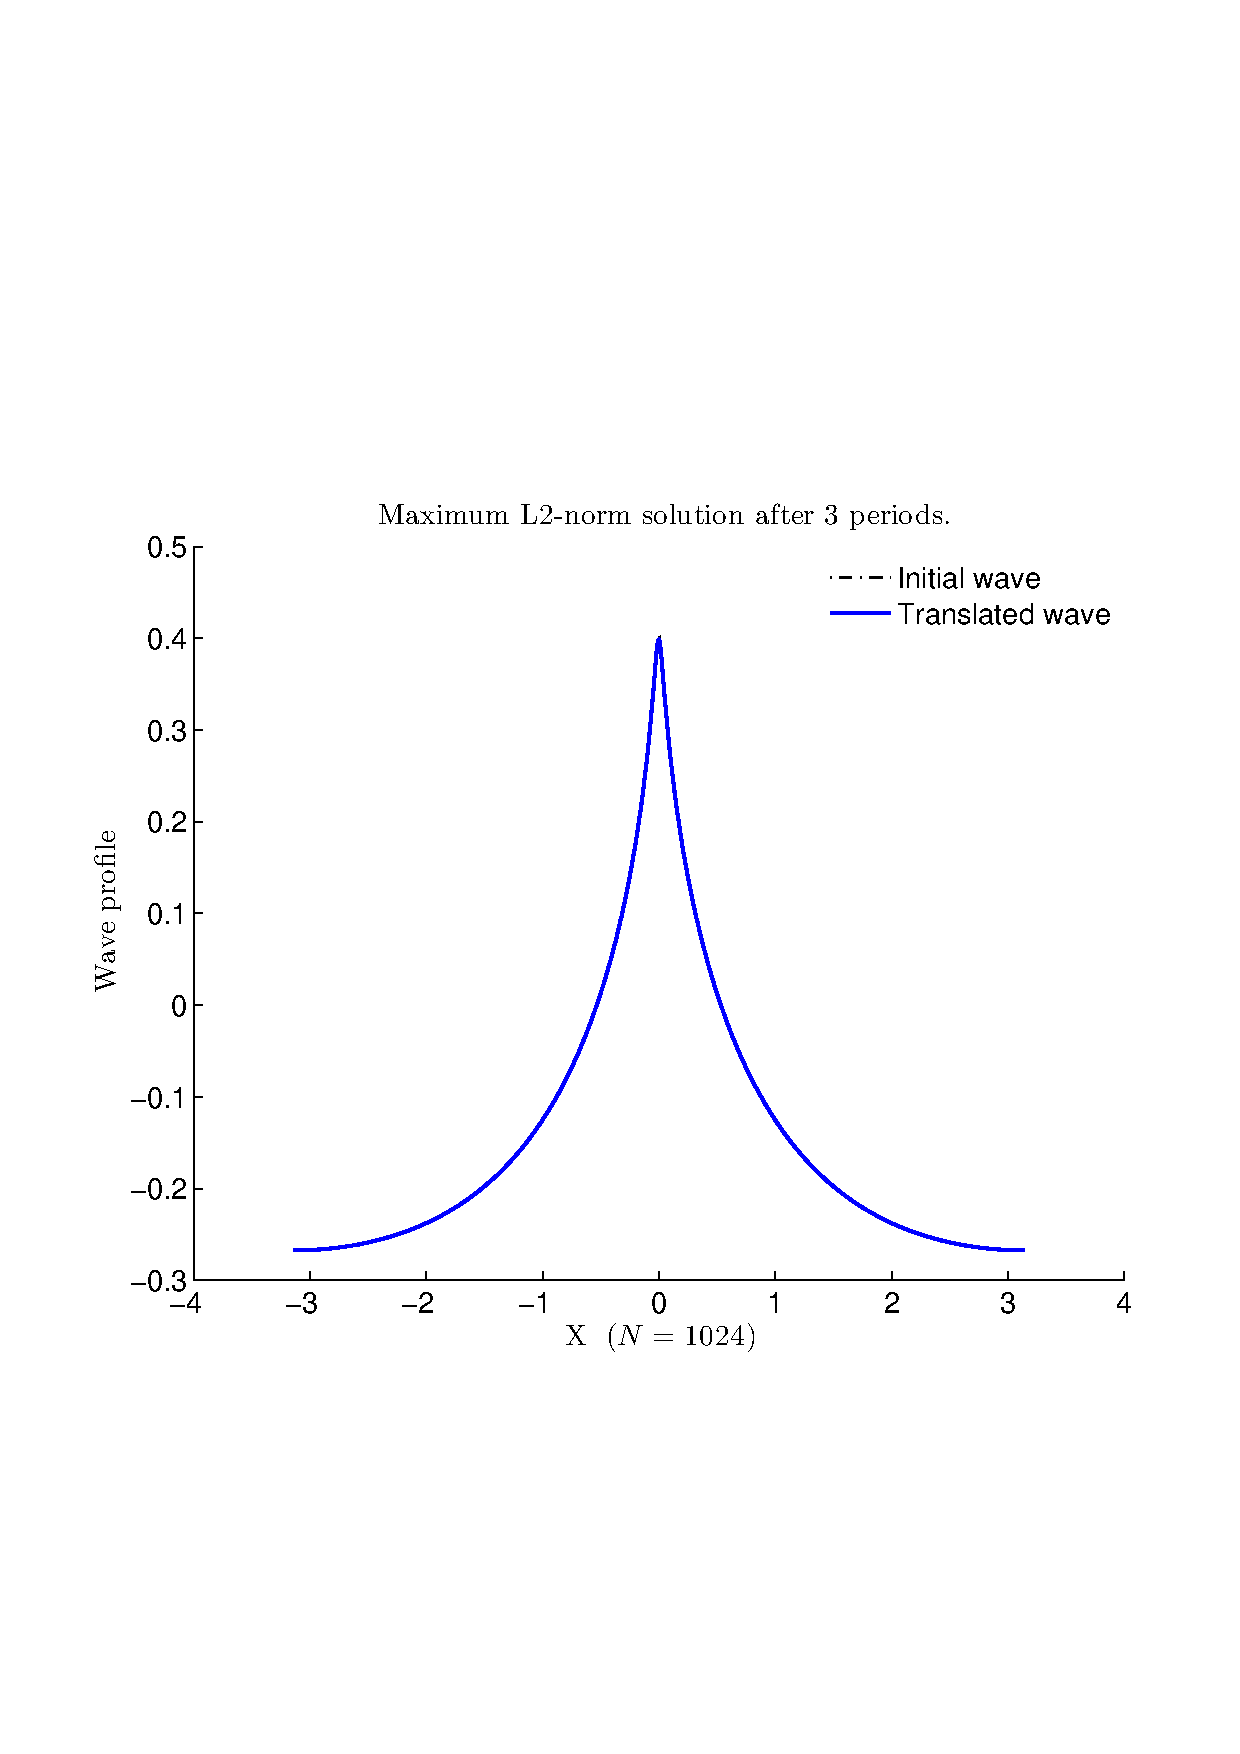
\includegraphics[scale=0.2, trim = 1.2cm 6.5cm 0.6cm 8cm, clip]{1024_full_3p_2.pdf}
%		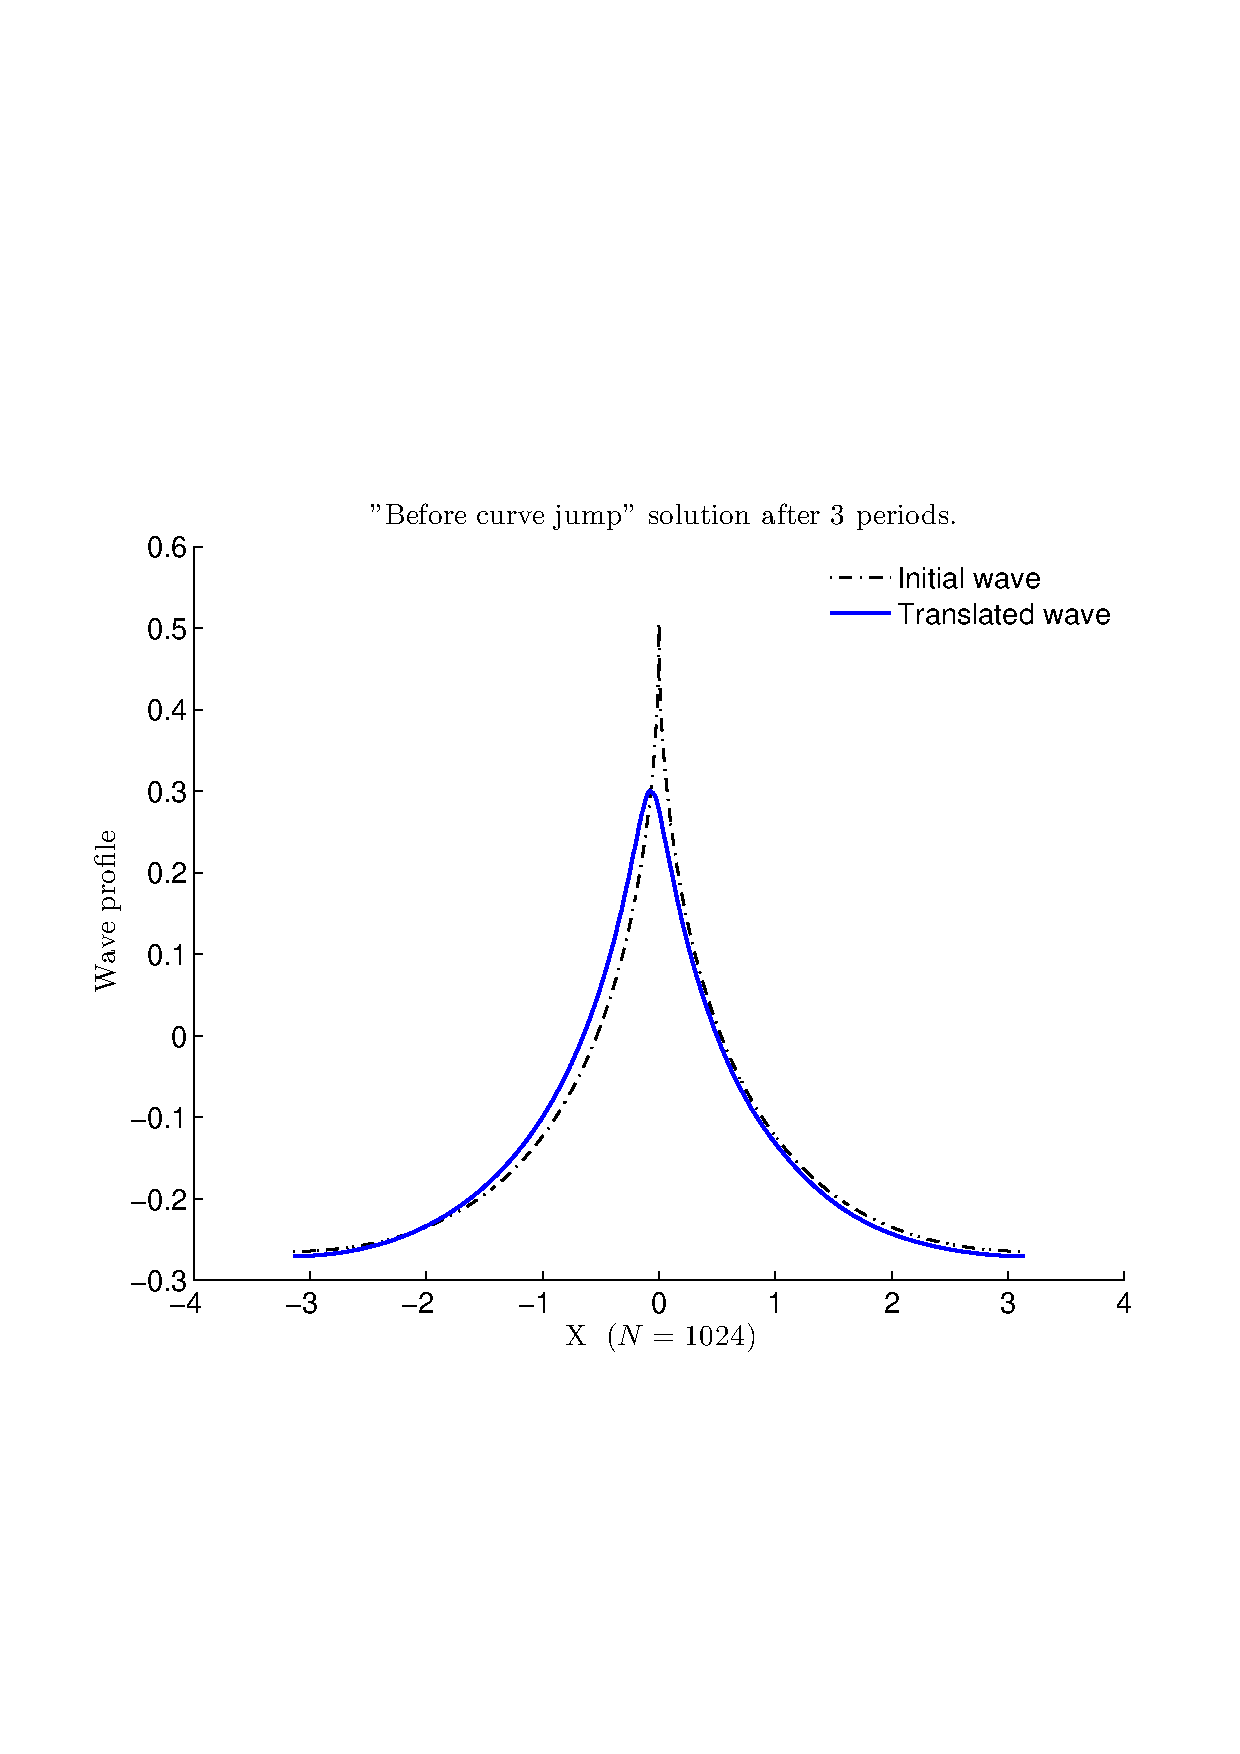
\includegraphics[scale=0.2, trim = 1.2cm 6.5cm 0.6cm 8cm, clip]{1024_full_3p_3.pdf}
%\end{figure}
\end{frame}
%%%%%%%%%%%%%%%%%%%%%%%%%%%%%%%%%%%%%%%%%%%%%%%%%%%%%%%%%%%%%%%%%%%%%%%%%%%%%
%%%%---------------------------------------------------------------------%%%%
%%%%%%%%%%%%%%%%%%%%%%%%%%%%%%%%%%%%%%%%%%%%%%%%%%%%%%%%%%%%%%%%%%%%%%%%%%%%%
\begin{frame}[t]{Stability of solutions: Whitham equation}
\centering{Whitham bifurcation curve ($\mbox{wavelength} = 2 \pi$). }
%	\begin{figure}[htbp]    
%		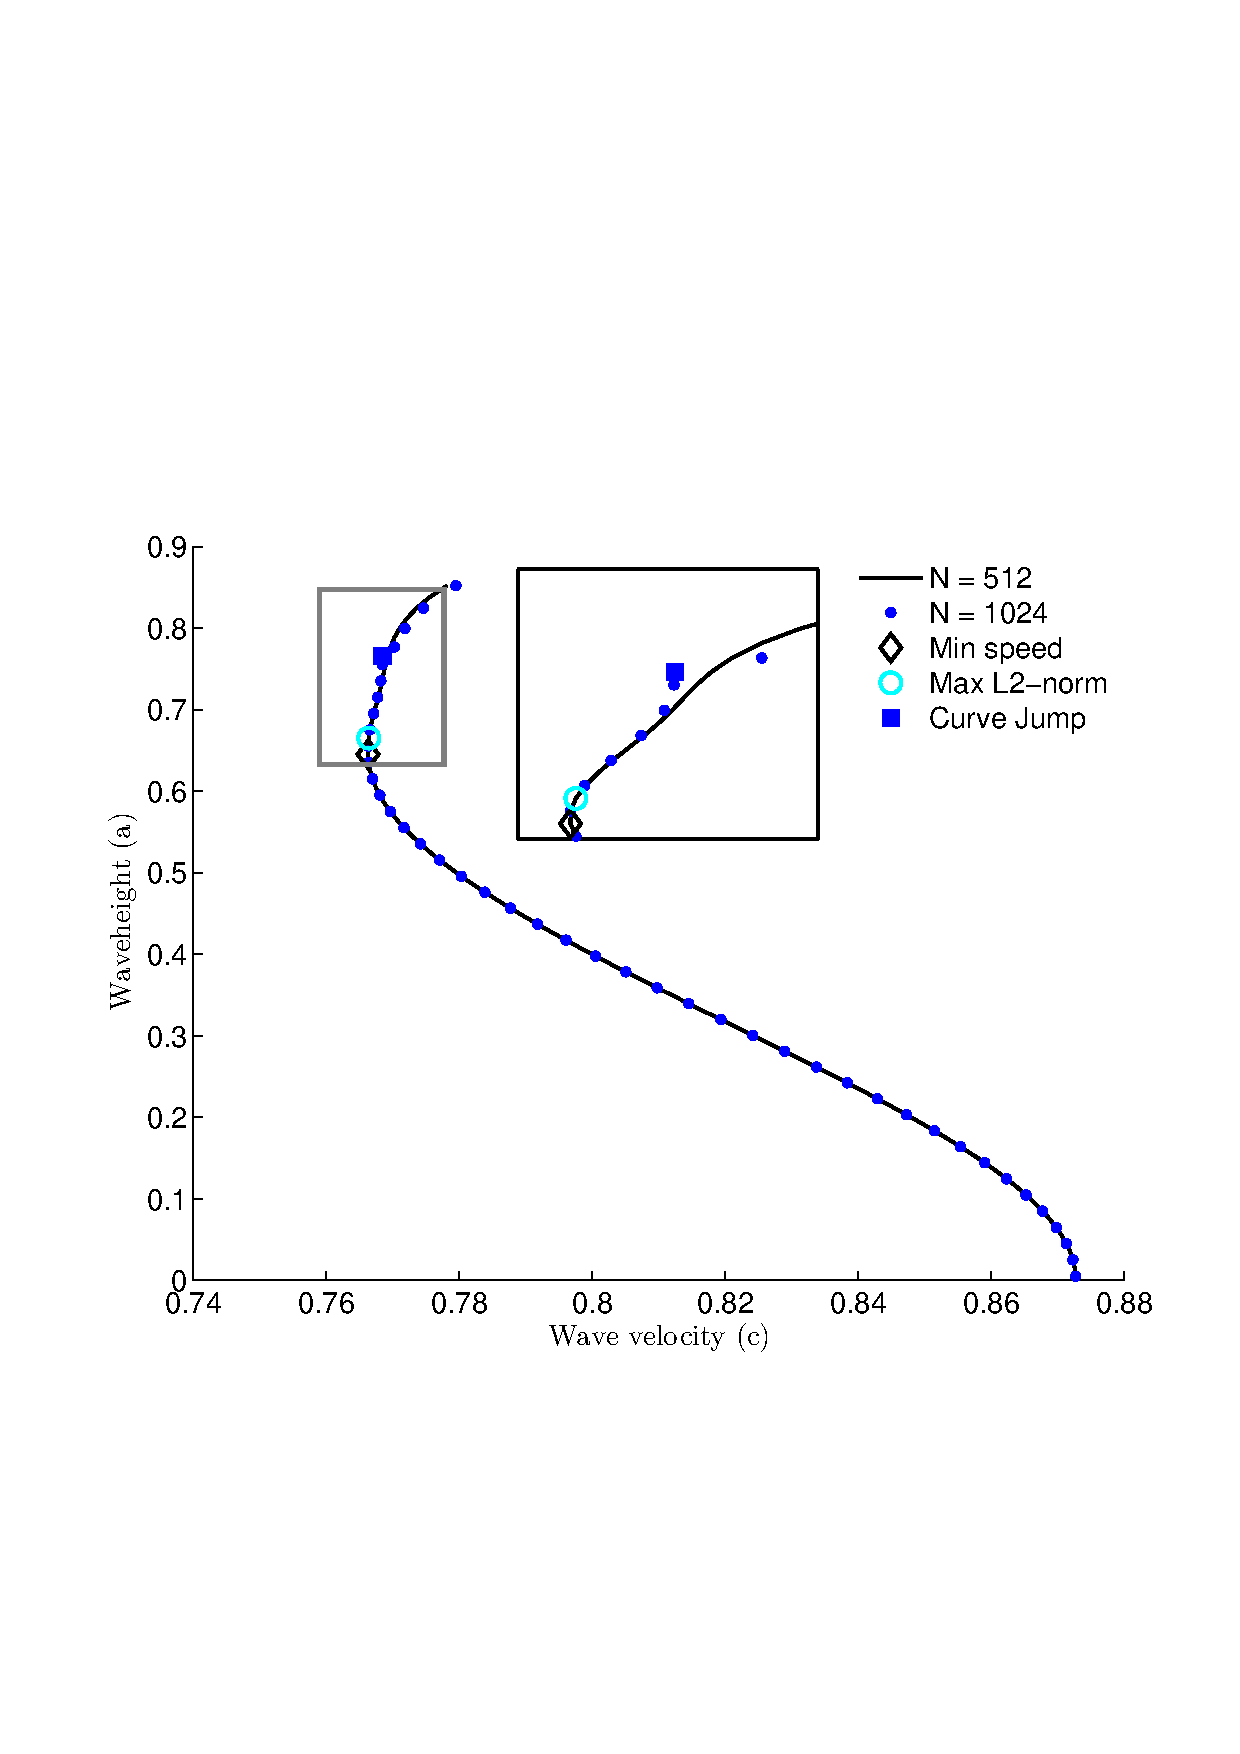
\includegraphics[scale=0.32, trim = 1.2cm 6.5cm 0.6cm 8cm, clip]{512_1024.pdf}
%		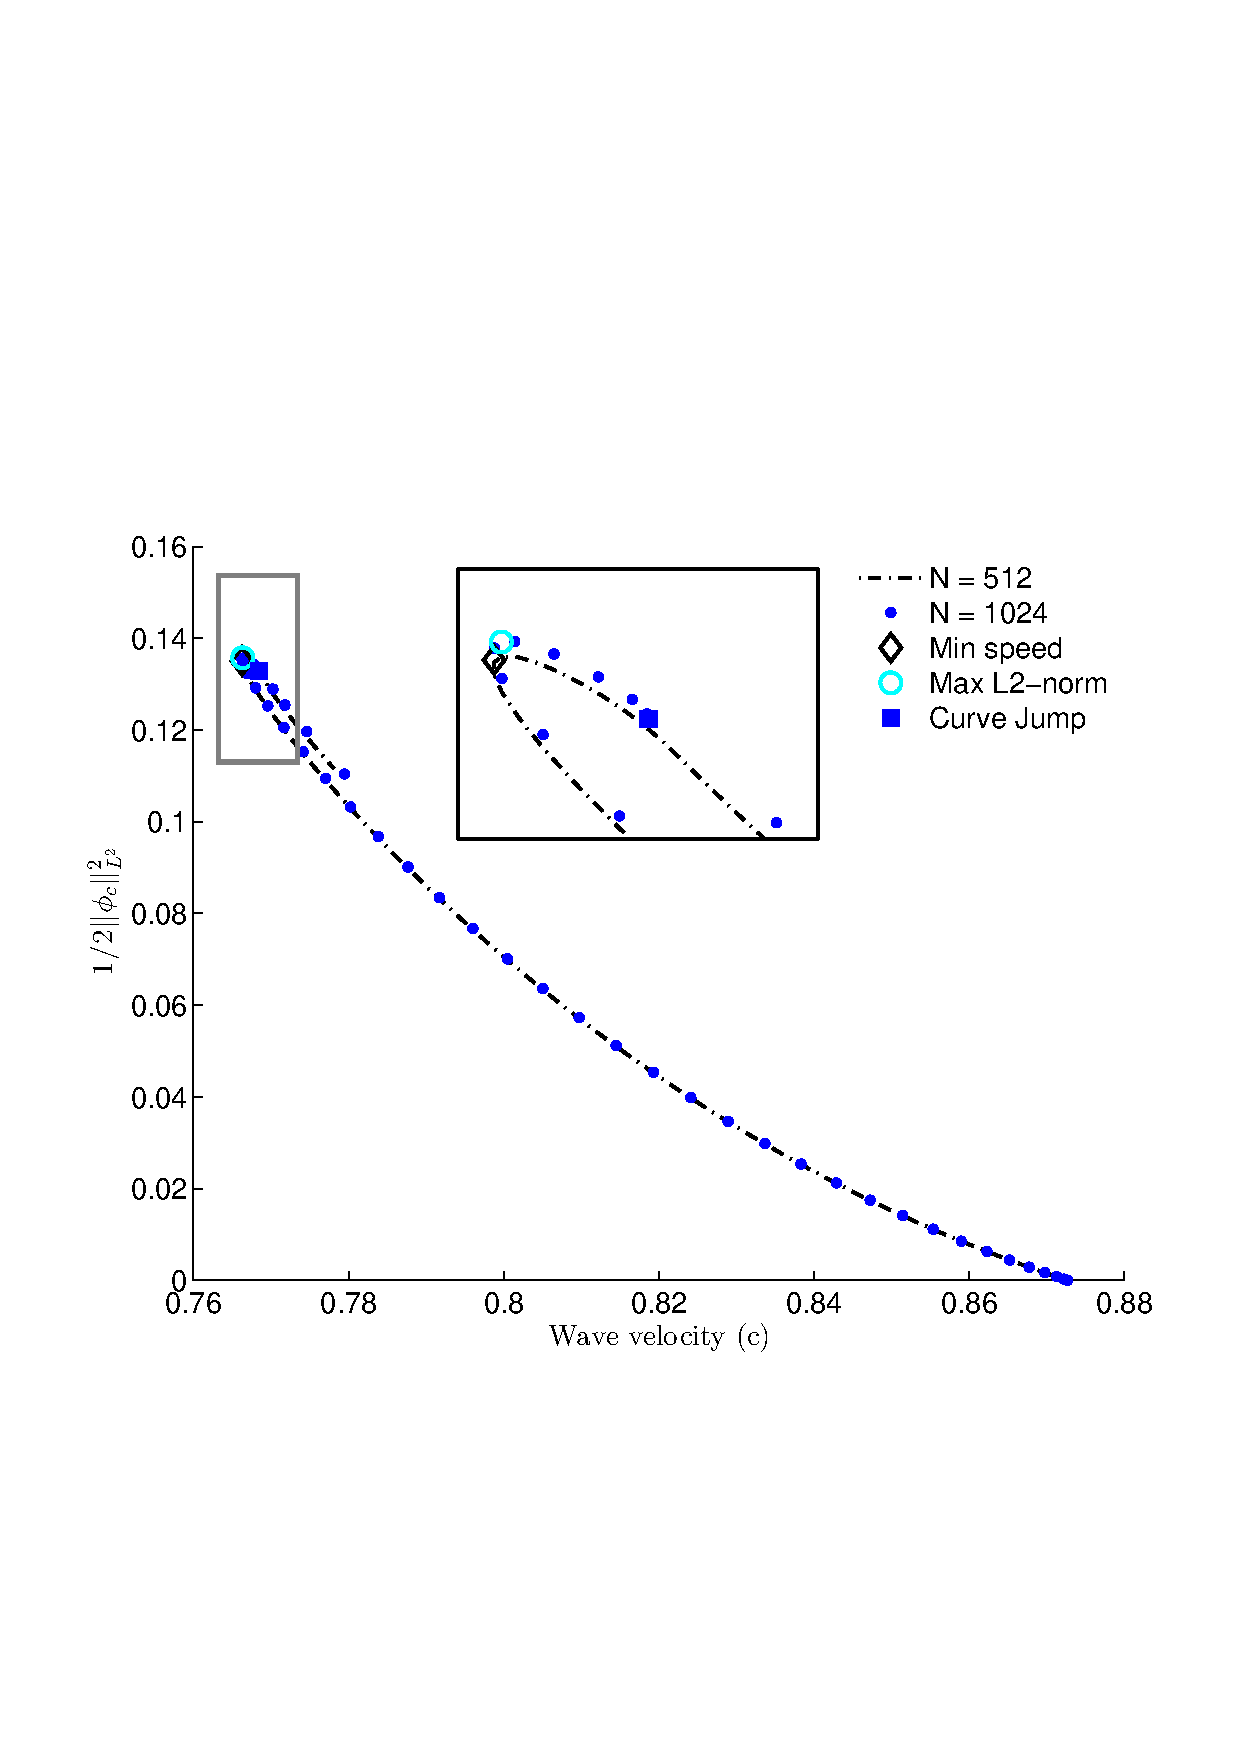
\includegraphics[scale=0.32, trim = 1.2cm 6.5cm 0.6cm 8cm, clip]{L2_512_1024.pdf}
%	\end{figure}
\end{frame}
%%%%%%%%%%%%%%%%%%%%%%%%%%%%%%%%%%%%%%%%%%%%%%%%%%%%%%%%%%%%%%%%%%%%%%%%%%%%%
%%%%---------------------------------------------------------------------%%%%
%%%%%%%%%%%%%%%%%%%%%%%%%%%%%%%%%%%%%%%%%%%%%%%%%%%%%%%%%%%%%%%%%%%%%%%%%%%%%
\begin{frame}[t]{Fitting spectral coefficients}
%\begin{figure}[htbp]    
%	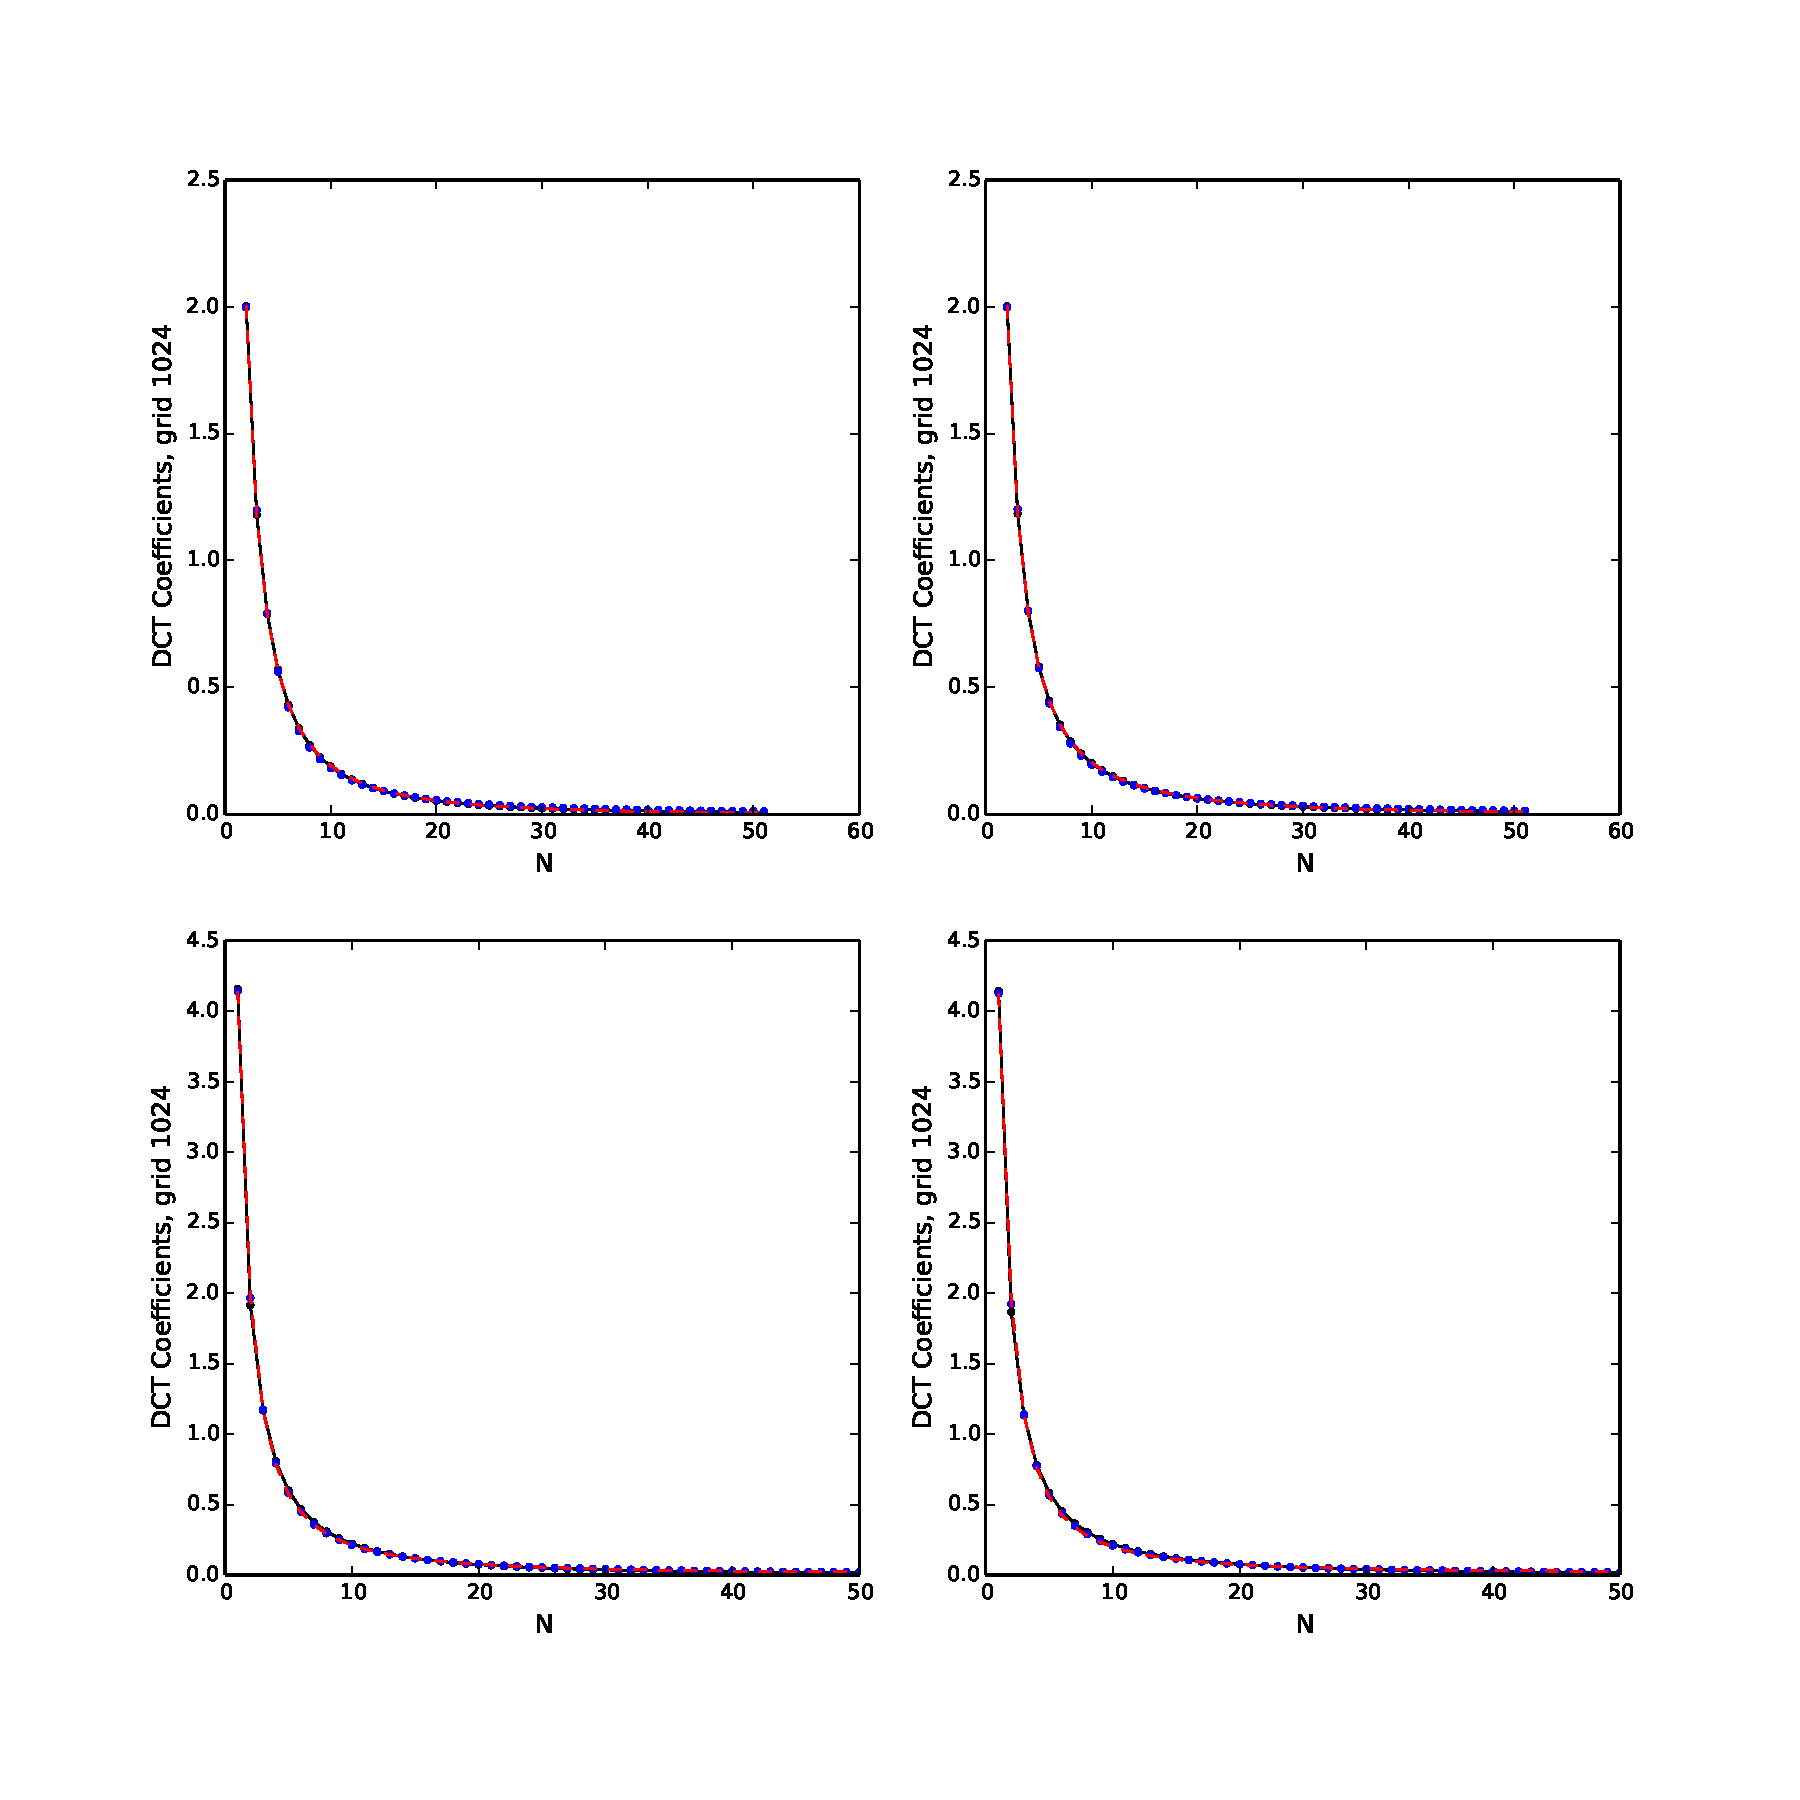
\includegraphics[scale=0.25]{spec_1024.pdf}
%	\caption{red dased line - spectral coefficients, black dash-dot-line - exponential fit, blue dotted line - polynomial fit.}
%\end{figure}
\end{frame}
%%%%%%%%%%%%%%%%%%%%%%%%%%%%%%%%%%%%%%%%%%%%%%%%%%%%%%%%%%%%%%%%%%%%%%%%%%%%%
%%%%---------------------------------------------------------------------%%%%
%%%%%%%%%%%%%%%%%%%%%%%%%%%%%%%%%%%%%%%%%%%%%%%%%%%%%%%%%%%%%%%%%%%%%%%%%%%%%
%\begin{frame}[t]{Fitting spectral coefficients}
%WAVE AT MINIMUM SPEED: 
%
%Exponential fit, grid 1024.
%
%L2 norm (residual) =  0.00021 $\qquad$ AIC = -467 $\qquad$ BIC = -461
% 
% 
%Polinomial fit, grid 1024.
% 
%L2 norm (residual) =  0.00255  $\qquad$ AIC = -344 $\qquad$ BIC = -337
%\noindent \newline 
% 
%WAVE WITH MAXIMUM L2 NORM: 
%
%Exponential fit, grid 1024.
%
%L2 norm (residual) =  0.00015 $\qquad$ AIC = -484 $\qquad$ BIC = -478
%
% 
%Polinomial fit, grid 1024.
% 
%L2 norm (residual) =  0.00175 $\qquad$ AIC = -363 $\qquad$ BIC = -355
%\noindent \newline 
% 
%WAVE BEFORE CURVE JUMP:
%
%Exponential fit, grid 1024.
%
%L2 norm (residual) =  0.00897 $\qquad$ AIC = -289 $\qquad$ BIC = -283
%
% 
%Polinomial fit, grid 1024.
%
%L2 norm (residual) =  0.00028 $\qquad$ AIC = -460 $\qquad$ BIC = -453
%\end{frame}
%%%%%%%%%%%%%%%%%%%%%%%%%%%%%%%%%%%%%%%%%%%%%%%%%%%%%%%%%%%%%%%%%%%%%%%%%%%%%%
%%%%%---------------------------------------------------------------------%%%%
%%%%%%%%%%%%%%%%%%%%%%%%%%%%%%%%%%%%%%%%%%%%%%%%%%%%%%%%%%%%%%%%%%%%%%%%%%%%%%
%\begin{frame}[t]{}
%\onslide<1-4>{
%
%
%\center{\Huge{Thank you for coming!}}
%
%}
%\onslide<2-4>{
%
%
%\center{\Huge{Have a safe trip back home!}}
%
%}
%
%\onslide<3-4>{
%
%\center{\Huge{Thank you for your attention!}}
%
%}
%
%\onslide<4-4>{
%
%\center{\Huge{Qs?}}
%
%}
%
%\end{frame}
